\documentclass[12pt, a4paper]{article}

%%%%% Packages

\usepackage{verbatim}
\usepackage[width=18.8cm, left=1.1cm, height=25.9cm, top=1.7cm]{geometry}
\usepackage{amsmath,graphicx}
\usepackage{amssymb, amsthm}
\usepackage{color, enumitem}
\usepackage{arcs} %\overarc{...} arc of circle
\usepackage{pifont}
\usepackage{soul}
\usepackage{wrapfig}
\usepackage{fancybox}
\usepackage{harpoon}
\usepackage{pgfplots}
\usepackage{tikz}
\usetikzlibrary{positioning}
\usetikzlibrary{shapes.multipart}
\usepackage{fancyhdr}
\pagestyle{fancy}
\renewcommand{\familydefault}{\rmdefault}
\usepackage{multicol}
\setlength{\parindent}{0cm}
\usepackage{fontspec} %加這個就可以設定字體
\usepackage{fourier}
\usepackage{cleveref}
\usepackage[most]{tcolorbox}
\usepackage{lipsum}
\usepackage[framemethod=TikZ]{mdframed}
\usepackage[hidelinks,hypertexnames=false]{hyperref}
\usepackage{xparse}
\usepackage{titlesec}
\usepackage{mathtools}


%%%%% Header and Footer

\renewcommand{\headrulewidth}{0pt}
\rhead{}

\cfoot{P. \thepage}

%%%%% Sbullet

\newcommand\sbullet[1][1]{\mathbin{\vcenter{\hbox{\scalebox{#1}{$\bullet$}}}}}


%%%%% Section Style

\titleformat{\section}
{\bf\LARGE}{\thesection.}{0.3em}{}


%%%%% MathsChris

\renewcommand{\MathsChris}{MathsChris\null}


%%%%% Recurring Decimals


\ExplSyntaxOn

%% Dots on the first and last digit
\NewDocumentCommand{\periodfl}{m}
{
  \repdec_initial_final_dots:n { #1 }
}

\seq_new:N \l__repdec_digits_seq
\tl_new:N \l__repdec_first_tl
\tl_new:N \l__repdec_last_tl

\cs_new_protected:Npn \repdec_initial_final_dots:n #1
{
  \seq_set_split:Nnn \l__repdec_digits_seq {} { #1 }
  \seq_pop_left:NN \l__repdec_digits_seq \l__repdec_first_tl
  \seq_pop_right:NN \l__repdec_digits_seq \l__repdec_last_tl
  \quark_if_no_value:VF \l__repdec_first_tl { \dot{\l__repdec_first_tl} }
  \seq_use:Nnnn \l__repdec_digits_seq {}{}{}
  \quark_if_no_value:VF \l__repdec_last_tl { \dot{\l__repdec_last_tl} }
}
\cs_generate_variant:Nn \quark_if_no_value:nF { V }

%% Dots on all digits
\NewDocumentCommand{\periodalldots}{m}
{
  \repdec_initial_all_dots:n { #1 }
}

\cs_new_protected:Npn \repdec_initial_all_dots:n #1
{
  \tl_map_inline:nn { #1 } { \dot{##1} }
}

%% Bar over period
\NewDocumentCommand{\periodbar}{m}
{
  \overline{ #1 }
}

%% Parentheses around period
\NewDocumentCommand{\periodparens}{m}
{
  (#1)
}

%% Dot on unique digit, bar on several digits
\NewDocumentCommand{\periodmixed}{m}
{
  \repdec_mixed:n { #1 }
}
\cs_new_protected:Npn \repdec_mixed:n #1
{
  \int_case:nnn { \tl_count:n { #1 } }
  {
    { 0 } { }
      { 1 } { \dot{#1} }
  }
  {
    \overline{#1}
  }
}

\ExplSyntaxOff

%%%%%






%%%%% enumitem setting
\setlistdepth{9}
\newlist{enumprob}{enumerate}{9}
\setenumerate[enumprob]{leftmargin=8mm,rightmargin=0pt,label=\arabic*.,labelwidth=8mm, itemsep=6mm, topsep=0mm, labelsep=2mm, labelindent=0pt, align=left, partopsep=5mm}
\setlist[enumprob,1]{label=\arabic*.,widest=999,itemindent=0pt,labelsep=2mm,labelwidth=6mm}
\setlist[enumprob,2]{label=(\alph*)}
\setlist[enumprob,3]{label=(\roman*)}
\setlist[enumprob,4]{label=(\arabic*)}
\setlist[enumprob,5]{label=(\arabic*)}
\setlist[enumprob,6]{label=(\arabic*)}
\setlist[enumprob,7]{label=(\arabic*)}
\setlist[enumprob,8]{label=(\arabic*)}
\setlist[enumprob,9]{label=(\arabic*)}



\setlistdepth{9}
\newlist{enumx}{enumerate}{9}
\setenumerate[enumx]{leftmargin=0.8cm,rightmargin=0pt,label=\arabic*.,labelwidth=6mm, itemsep=3pt, topsep=3mm, labelsep=2mm, labelindent=0pt, align=left, partopsep=0mm}
\setlist[enumx,1]{label=\arabic*.}
\setlist[enumx,2]{label=(\alph*),itemsep=0pt,topsep=0pt}
\setlist[enumx,3]{label=(\roman*)}
\setlist[enumx,4]{label=(\arabic*)}
\setlist[enumx,5]{label=(\arabic*)}
\setlist[enumx,6]{label=(\arabic*)}
\setlist[enumx,7]{label=(\arabic*)}
\setlist[enumx,8]{label=(\arabic*)}
\setlist[enumx,9]{label=(\arabic*)}


\setlistdepth{9}
\newlist{thinkitem}{enumerate}{9}
\setenumerate[thinkitem]{leftmargin=1.2em,rightmargin=0pt,label=\textcolor{green!80!black}{\sbullet[1.5]},itemsep=0pt,topsep=3pt}

\newlist{itemlist}{enumerate}{9}
\setenumerate[itemlist]{leftmargin=1.2em,rightmargin=0pt,label={\sbullet[1.5]},itemsep=0pt,topsep=3pt}

\setlistdepth{9}
\newlist{planitem}{enumerate}{9}
\setenumerate[planitem]{leftmargin=*,rightmargin=0pt,label=\arabic*.,itemsep=0pt,topsep=3pt,widest=99}
\setlist[planitem,1]{label=\arabic*.}
\setlist[planitem,2]{label=(\alph*)}
\setlist[planitem,3]{label=(\roman*)}
\setlist[planitem,4]{label=(\arabic*)}
\setlist[planitem,5]{label=(\arabic*)}
\setlist[planitem,6]{label=(\arabic*)}
\setlist[planitem,7]{label=(\arabic*)}
\setlist[planitem,8]{label=(\arabic*)}
\setlist[planitem,9]{label=(\arabic*)}

\newlist{steps}{enumerate}{9}
\setenumerate[steps]{leftmargin=*,rightmargin=0pt,label=Step~\arabic*.,itemsep=0pt,topsep=3pt,widest=99}
\setlist[steps,1]{label=Step \arabic*.}
\setlist[steps,2]{label=(\alph*)}
\setlist[steps,3]{label=(\roman*)}
\setlist[steps,4]{label=(\arabic*)}
\setlist[steps,5]{label=(\arabic*)}
\setlist[steps,6]{label=(\arabic*)}
\setlist[steps,7]{label=(\arabic*)}
\setlist[steps,8]{label=(\arabic*)}
\setlist[steps,9]{label=(\arabic*)}

\newlist{writesteps}{enumerate}{9}
\setenumerate[writesteps]{leftmargin=*,rightmargin=0pt,label={\small \tt \textcolor{blue}{\arabic*.}},itemsep=0pt,topsep=3pt,widest=99}
\setlist[writesteps,1]{label={\small \tt \textcolor{blue}{\arabic*.}}}
\setlist[writesteps,2]{label={\small \tt \textcolor{blue}{(\alph*)}}}
\setlist[writesteps,3]{label=(\roman*)}
\setlist[writesteps,4]{label=(\arabic*)}
\setlist[writesteps,5]{label=(\arabic*)}
\setlist[writesteps,6]{label=(\arabic*)}
\setlist[writesteps,7]{label=(\arabic*)}
\setlist[writesteps,8]{label=(\arabic*)}
\setlist[writesteps,9]{label=(\arabic*)}

\newcommand{\planstep}[1]{\ensuremath{\text{\small \tt \textcolor{blue}{[#1]}}}}




%%%%% Fonts Setting
\setmainfont{Times New Roman}
\usepackage{xeCJK}  %讓中英文字體分開設置
\setCJKmainfont{新細明體} %設定中文為系統上的字型,而英文不去更動,使用原TeX字%型
\XeTeXlinebreaklocale "zh"   %這兩行一定要加,中文才能自動換行
\XeTeXlinebreakskip = 0pt plus 1pt %這兩行一定要加,中文才能自動換行

%%%%% User Defined Functions
\newcommand{\abs}[1]{\left|#1\right|}
\newcommand{\dps}{\displaystyle}
\newcommand{\parallelsum}{\mathbin{\!/\mkern-5mu/\!}}
\renewcommand{\overarc}[1]{\widearc{#1}}
\newcommand{\any}{\forall\, }
\newcommand{\degree}{\ensuremath{^{\circ}}}
\renewcommand{\d}{\mbox{d}}

\newcommand{\NF}{
  \begin{tikzpicture}
    \node[inner sep=0.1cm, preaction={fill=black,fill opacity=0.15},rounded corners=0.1ex,font=\fontsize{7pt}{17pt}\selectfont] (c) {\textbf{NF}}
  \end{tikzpicture}
}

%%% Vectors
\renewcommand{\i}{\mathbf{i}}
\renewcommand{\j}{\mathbf{j}}
\renewcommand{\k}{\mathbf{k}}
\renewcommand{\vec}[1]{\overrightharp{#1}}

%%%%% Marking Style
\renewcommand{\marks}[1]{\hfill\null\hfill (#1~marks)}
\newcommand{\onemark}{\hfill\null\hfill (1~mark)}

%%%%% Graphics

\newcommand{\graphics}[1]{\par
  \begin{center}
    \includegraphics{#1}
  \end{center}
}

\graphicspath{{D:/DSEbyTopic/Graphics/}}

\newcommand{\mcgraphics}[2]{
  \null\par
  \vspace{-3mm}
  \begin{minipage}[t]{0.45\textwidth}

    #2

  \end{minipage}
  \begin{minipage}[t]{0.5\textwidth}
    \null\par
    \vspace{-0.02\textwidth}

    \begin{flushright}
      \includegraphics{#1}
    \end{flushright}
  \end{minipage}
  \vspace{0.01\textwidth}
}


%%%%% Environments

\newenvironment{absolutelynopagebreak}
{\nobreak\vfil\penalty0\vfilneg
  \vtop\bgroup}
{\par\xdef\tpd{\the\prevdepth}\egroup
  \prevdepth=\tpd}

\newcommand{\greybox}[1]{
  \begin{tikzpicture}
    \node[inner sep=0.3cm, preaction={fill=black,fill opacity=0.15},rounded corners=1ex,font=\fontsize{24pt}{24pt}\selectfont] (c) {#1}
  \end{tikzpicture}
}

\SetLabelAlign{parright}{\parbox[t]{\labelwidth}{\raggedleft‌​#1}}


%%%%% get and put

\newcommand{\sectiontitle}[3]{\input{"D:/DSEbyTopic/SectionTitle/Title_#1_#2_#3.tex"}}


\newcommand{\problem}[2][]{
  \begin{minipage}[t]{(\textwidth-1cm)}
    \input{"D:/DSEbyTopic/Problems/#2.tex"}%
    \ifstrempty{#1}%
    {
    }%
    {\linebreak\null\hfill[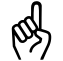
\includegraphics{uppointing}#2]
    }%
  \end{minipage}
}



\newcommand{\problemans}[1]{
  \begin{minipage}[t]{(\textwidth-1cm)}
    \input{"D:/DSEbyTopic/Problems/#1-ans.tex"}
  \end{minipage}
}


%%%%% Graphics


\newcommand{\starr}{
\includegraphics{star}}

\graphicspath{{D:/DSEbyTopic/Graphics/}}

\newcommand{\mcgraphics}[2]{
  \par
  \vspace{0.0001\textwidth}
  \begin{minipage}[t]{0.33\textwidth}

    #2

  \end{minipage}
  \begin{minipage}[t]{0.65\textwidth}
    \null\par
    \vspace{-0.12\textwidth}

    \begin{flushright}
      \includegraphics{#1}
    \end{flushright}
  \end{minipage}
  \vspace{0.01\textwidth}
}



%%%%% environment commands


%%%%% TC environment

\newcounter{tccounter}
\setcounter{tccounter}{0}
\renewcommand{\thetccount}{\arabic{tccounter}}
\newenvironment{theorem}[2][]{%
  \refstepcounter{tccounter}%
  \ifstrempty{#1}%
  {\mdfsetup{%
      frametitle={%
          \tikz[baseline=(current bounding box.east),outer sep=0pt]
          \node[anchor=east,rectangle,fill=blue!20]
          {\strut Theorem~\thetccount};}}
  }%
  {\mdfsetup{%
      frametitle={%
          \tikz[baseline=(current bounding box.east),outer sep=0pt]
          \node[anchor=east,rectangle,fill=blue!20]
          {\strut Theorem~\thetccount~(#1)~};}}%
  }%
  \mdfsetup{innertopmargin=4pt,innerbottommargin=10pt,linecolor=blue!20,%
    linewidth=2pt,topline=true,%
    frametitleaboveskip=\dimexpr-\ht\strutbox\relax
  }
  \begin{mdframed}[]\relax%
    \label{#2}}{\end{mdframed}}

\newenvironment{concept}[2][]{%
  \refstepcounter{tccounter}%
  \ifstrempty{#1}%
  {\mdfsetup{%
      frametitle={%
          \tikz[baseline=(current bounding box.east),outer sep=0pt]
          \node[anchor=east,rectangle,fill=blue!20]
          {\strut Concept~\thetccount};}}
  }%
  {\mdfsetup{%
      frametitle={%
          \tikz[baseline=(current bounding box.east),outer sep=0pt]
          \node[anchor=east,rectangle,fill=blue!20]
          {\strut Concept~\thetccount~(#1)~};}}%
  }%
  \mdfsetup{innertopmargin=4pt,innerbottommargin=10pt,linecolor=blue!20,%
    linewidth=2pt,topline=true,%
    frametitleaboveskip=\dimexpr-\ht\strutbox\relax
  }
  \begin{mdframed}[]\relax%
    \label{#2}}{\end{mdframed}}

\newenvironment{formula}[2][]{%
  \refstepcounter{tccounter}%
  \ifstrempty{#1}%
  {\mdfsetup{%
      frametitle={%
          \tikz[baseline=(current bounding box.east),outer sep=0pt]
          \node[anchor=east,rectangle,fill=blue!20]
          {\strut Formula~\thetccount};}}
  }%
  {\mdfsetup{%
      frametitle={%
          \tikz[baseline=(current bounding box.east),outer sep=0pt]
          \node[anchor=east,rectangle,fill=blue!20]
          {\strut Formula~\thetccount~(#1)~};}}%
  }%
  \mdfsetup{innertopmargin=4pt,innerbottommargin=10pt,linecolor=blue!20,%
    linewidth=2pt,topline=true,%
    frametitleaboveskip=\dimexpr-\ht\strutbox\relax
  }
  \begin{mdframed}[]\relax%
    \label{#2}}{\end{mdframed}}


\newenvironment{presentation}[2][]{%
  \refstepcounter{tccounter}%
  \ifstrempty{#1}%
  {\mdfsetup{%
      frametitle={%
          \tikz[baseline=(current bounding box.east),outer sep=0pt]
          \node[anchor=east,rectangle,fill=blue!20]
          {\strut Presentation~\thetccount};}}
  }%
  {\mdfsetup{%
      frametitle={%
          \tikz[baseline=(current bounding box.east),outer sep=0pt]
          \node[anchor=east,rectangle,fill=blue!20]
          {\strut Presentation~\thetccount~(#1)~};}}%
  }%
  \mdfsetup{innertopmargin=4pt,innerbottommargin=10pt,linecolor=blue!20,%
    linewidth=2pt,topline=true,%
    frametitleaboveskip=\dimexpr-\ht\strutbox\relax
  }
  \begin{mdframed}[]\relax%
    \label{#2}}{\end{mdframed}}


%%%%% LP environment

\newcounter{lpcounter}
\setcounter{lpcounter}{0}
\renewcommand{\thelpcount}{\arabic{lpcounter}}

\newenvironment{skill}[2][]{%
  \refstepcounter{lpcounter}%
  \ifstrempty{#1}%
  {\mdfsetup{%
      frametitle={%
          \tikz[baseline=(current bounding box.east),outer sep=0pt]
          \node[anchor=east,rectangle,fill=red!20]
          {\strut Skill~\thelpcount};}}
  }%
  {\mdfsetup{%
      frametitle={%
          \tikz[baseline=(current bounding box.east),outer sep=0pt]
          \node[anchor=east,rectangle,fill=red!20]
          {\strut Skill~\thelpcount~(#1)~};}}%
  }%
  \mdfsetup{innertopmargin=4pt,innerbottommargin=10pt,linecolor=red!20,%
    linewidth=2pt,topline=true,%
    frametitleaboveskip=\dimexpr-\ht\strutbox\relax
  }
  \begin{mdframed}[]\relax%
    \label{#2}}{\end{mdframed}}


\newenvironment{trick}[2][]{%
  \refstepcounter{lpcounter}%
  \ifstrempty{#1}%
  {\mdfsetup{%
      frametitle={%
          \tikz[baseline=(current bounding box.east),outer sep=0pt]
          \node[anchor=east,rectangle,fill=red!20]
          {\strut Trick~\thelpcount};}}
  }%
  {\mdfsetup{%
      frametitle={%
          \tikz[baseline=(current bounding box.east),outer sep=0pt]
          \node[anchor=east,rectangle,fill=red!20]
          {\strut Trick~\thelpcount~(#1)~};}}%
  }%
  \mdfsetup{innertopmargin=4pt,innerbottommargin=10pt,linecolor=red!20,%
    linewidth=2pt,topline=true,%
    frametitleaboveskip=\dimexpr-\ht\strutbox\relax
  }
  \begin{mdframed}[]\relax%
    \label{#2}}{\end{mdframed}}


\newenvironment{fact}[2][]{%
  \refstepcounter{lpcounter}%
  \ifstrempty{#1}%
  {\mdfsetup{%
      frametitle={%
          \tikz[baseline=(current bounding box.east),outer sep=0pt]
          \node[anchor=east,rectangle,fill=red!20]
          {\strut Fact~\thelpcount};}}
  }%
  {\mdfsetup{%
      frametitle={%
          \tikz[baseline=(current bounding box.east),outer sep=0pt]
          \node[anchor=east,rectangle,fill=red!20]
          {\strut Fact~\thelpcount~(#1)~};}}%
  }%
  \mdfsetup{innertopmargin=4pt,innerbottommargin=10pt,linecolor=red!20,%
    linewidth=2pt,topline=true,%
    frametitleaboveskip=\dimexpr-\ht\strutbox\relax
  }
  \begin{mdframed}[]\relax%
    \label{#2}}{\end{mdframed}}


\newenvironment{skillgroup}[2][]{%
  \refstepcounter{lpcounter}%
  \ifstrempty{#1}%
  {\mdfsetup{%
      frametitle={%
          \tikz[baseline=(current bounding box.east),outer sep=0pt]
          \node[anchor=east,rectangle,fill=red!20]
          {\strut Skill Group~\thelpcount};}}
  }%
  {\mdfsetup{%
      frametitle={%
          \tikz[baseline=(current bounding box.east),outer sep=0pt]
          \node[anchor=east,rectangle,fill=red!20]
          {\strut Skill Group~\thelpcount~(#1)~};}}%
  }%
  \mdfsetup{innertopmargin=4pt,innerbottommargin=10pt,linecolor=red!20,%
    linewidth=2pt,topline=true,%
    frametitleaboveskip=\dimexpr-\ht\strutbox\relax
  }
  \begin{mdframed}[]\relax%
    \label{#2}}{\end{mdframed}}


\newenvironment{trickgroup}[2][]{%
  \refstepcounter{lpcounter}%
  \ifstrempty{#1}%
  {\mdfsetup{%
      frametitle={%
          \tikz[baseline=(current bounding box.east),outer sep=0pt]
          \node[anchor=east,rectangle,fill=red!20]
          {\strut Trick Group~\thelpcount};}}
  }%
  {\mdfsetup{%
      frametitle={%
          \tikz[baseline=(current bounding box.east),outer sep=0pt]
          \node[anchor=east,rectangle,fill=red!20]
          {\strut Trick Group~\thelpcount~(#1)~};}}%
  }%
  \mdfsetup{innertopmargin=4pt,innerbottommargin=10pt,linecolor=red!20,%
    linewidth=2pt,topline=true,%
    frametitleaboveskip=\dimexpr-\ht\strutbox\relax
  }
  \begin{mdframed}[]\relax%
    \label{#2}}{\end{mdframed}}


\newenvironment{factgroup}[2][]{%
  \refstepcounter{lpcounter}%
  \ifstrempty{#1}%
  {\mdfsetup{%
      frametitle={%
          \tikz[baseline=(current bounding box.east),outer sep=0pt]
          \node[anchor=east,rectangle,fill=red!20]
          {\strut Fact Group~\thelpcount};}}
  }%
  {\mdfsetup{%
      frametitle={%
          \tikz[baseline=(current bounding box.east),outer sep=0pt]
          \node[anchor=east,rectangle,fill=red!20]
          {\strut Fact Group~\thelpcount~(#1)~};}}%
  }%
  \mdfsetup{innertopmargin=4pt,innerbottommargin=10pt,linecolor=red!20,%
    linewidth=2pt,topline=true,%
    frametitleaboveskip=\dimexpr-\ht\strutbox\relax
  }
  \begin{mdframed}[]\relax%
    \label{#2}}{\end{mdframed}}

\newenvironment{pattern}[2][]{%
  \refstepcounter{lpcounter}%
  \ifstrempty{#1}%
  {\mdfsetup{%
      frametitle={%
          \tikz[baseline=(current bounding box.east),outer sep=0pt]
          \node[anchor=east,rectangle,fill=red!20]
          {\strut Pattern~\thelpcount};}}
  }%
  {\mdfsetup{%
      frametitle={%
          \tikz[baseline=(current bounding box.east),outer sep=0pt]
          \node[anchor=east,rectangle,fill=red!20]
          {\strut Pattern~\thelpcount~(#1)~};}}%
  }%
  \mdfsetup{innertopmargin=4pt,innerbottommargin=10pt,linecolor=red!20,%
    linewidth=2pt,topline=true,%
    frametitleaboveskip=\dimexpr-\ht\strutbox\relax
  }
  \begin{mdframed}[]\relax%
    \label{#2}}{\end{mdframed}}


\newcounter{illucounter}[lpcounter]
\setcounter{illucounter}{0}
\renewcommand{\theillucounter}{\thelpcounter.\arabic{illucounter}}

\newenvironment{illustration}[2][]{%
  \refstepcounter{illucounter}%
  \ifstrempty{#1}%
  {\mdfsetup{%
      frametitle={%
          \tikz[baseline=(current bounding box.east),outer sep=0pt]
          \node[anchor=east,rectangle,fill=red!10]
          {\strut Illustration~\theillucounter};}}
  }%
  {\mdfsetup{%
      frametitle={%
          \tikz[baseline=(current bounding box.east),outer sep=0pt]
          \node[anchor=east,rectangle,fill=red!10]
          {\strut Illustration~\theillucounter~(#1)~};}}%
  }%
  \mdfsetup{innertopmargin=4pt,innerbottommargin=10pt,linecolor=red!10,%
    linewidth=2pt,topline=true,%
    frametitleaboveskip=\dimexpr-\ht\strutbox\relax
  }
  \begin{mdframed}[]\relax%
    \label{#2}}{\end{mdframed}}

\newenvironment{tiy}[2][]{%
  \refstepcounter{illucounter}%
  \ifstrempty{#1}%
  {\mdfsetup{%
      frametitle={%
          \tikz[baseline=(current bounding box.east),outer sep=0pt]
          \node[anchor=east,rectangle,fill=red!20]
          {\strut Try it Yourself~\theillucounter};}}
  }%
  {\mdfsetup{%
      frametitle={%
          \tikz[baseline=(current bounding box.east),outer sep=0pt]
          \node[anchor=east,rectangle,fill=red!20]
          {\strut Try it Yourself~\theillucounter~(#1)~};}}%
  }%
  \mdfsetup{innertopmargin=4pt,innerbottommargin=10pt,linecolor=red!20,%
    linewidth=2pt,topline=true,%
    frametitleaboveskip=\dimexpr-\ht\strutbox\relax
  }
  \begin{mdframed}[]\relax%
    \label{#2}}{\end{mdframed}}



%%%%% Eg Environments

\newcounter{egcounter}
\setcounter{egcounter}{0}
\renewcommand{\theegcount}{\arabic{egcounter}}
\newenvironment{example}[2][]{%
  \begin{absolutelynopagebreak}
    \refstepcounter{egcounter}%
    \ifstrempty{#1}%
    {\mdfsetup{%
        frametitle={%
            \tikz[baseline=(current bounding box.east),outer sep=0pt]
            \node[anchor=east,rectangle,fill=green!40]
            {\strut Example~\theegcount};}}
    }%
    {\mdfsetup{%
        frametitle={%
            \tikz[baseline=(current bounding box.east),outer sep=0pt]
            \node[anchor=east,rectangle,fill=green!40]
            {\strut Example~\theegcount~(#1)~};}}%
    }%
    \mdfsetup{innertopmargin=4pt,innerbottommargin=10pt,linecolor=green!40,%
      linewidth=2pt,topline=true,%
      frametitleaboveskip=\dimexpr-\ht\strutbox\relax,
      skipabove=0pt,skipbelow=25pt,
    }
    \begin{mdframed}[]\relax%
      \label{#2}}{\end{mdframed}\end{absolutelynopagebreak}}


\newenvironment{Question}[2][]{%
  \begin{absolutelynopagebreak}
    \refstepcounter{egcounter}%
    \ifstrempty{#1}%
    {\mdfsetup{%
        frametitle={%
            \tikz[baseline=(current bounding box.east),outer sep=0pt]
            \node[anchor=east,rectangle,fill=green!40]
            {\strut Example~\ref{#2}};}}
    }%
    {\mdfsetup{%
        frametitle={%
            \tikz[baseline=(current bounding box.east),outer sep=0pt]
            \node[anchor=east,rectangle,fill=green!40]
            {\strut Example~\ref{#2}~(#1)~};}}%
    }%
    \mdfsetup{innertopmargin=4pt,innerbottommargin=10pt,linecolor=green!40,%
      linewidth=2pt,topline=true,%
      frametitleaboveskip=\dimexpr-\ht\strutbox\relax,
      skipabove=0pt,skipbelow=25pt,
    }
    \begin{mdframed}[]\relax%
      }{\end{mdframed}\end{absolutelynopagebreak}}






\newenvironment{Read}{%
  \begin{mdframed}[%
      frametitle={
\includegraphics{Read}~Read the Question},
      apptotikzsetting={\tikzset{mdfframetitlebackground/.append style={%
              shade,left color=green!20!white, right color=white}}},
      %frametitlerule=true,
      %frametitlerulewidth=1pt,
      %frametitlerulecolor=black,
      innertopmargin=0.7em,%
      innerleftmargin=0.7em,%,
      innerrightmargin=0.7em,
      hidealllines=true,leftline=true,
      frametitlebackgroundcolor=green!20,
      linewidth=3pt,
      linecolor=green!20,
      skipabove=0pt,skipbelow=0pt,
      %fontcolor=white,%
      %backgroundcolor=green!10
    ]%
    }{%
  \end{mdframed}
}

\newcommand{\readrule}{\textcolor{green!80!black}{\hrulefill}}
\newcommand{\illustrationrule}{\textcolor{red!10}{\hrulefill}}



\newenvironment{Think}{%
  \begin{mdframed}[%
      frametitle={
\includegraphics{Think}~Thinking Process},
      apptotikzsetting={\tikzset{mdfframetitlebackground/.append style={%
              shade,left color=green!20!white, right color=white}}},
      %frametitlerule=true,
      %frametitlerulewidth=1pt,
      %frametitlerulecolor=black,
      innertopmargin=0.7em,%
      innerleftmargin=0.7em,%,
      innerrightmargin=0.7em,
      hidealllines=true,leftline=true,
      frametitlebackgroundcolor=green!20,
      linewidth=3pt,
      linecolor=green!20,
      skipabove=0pt,skipbelow=0pt,
      %fontcolor=white,%
      %backgroundcolor=green!10
    ]%
    }{%
  \end{mdframed}
}

\newenvironment{Plan}{%
  \begin{mdframed}[%
      frametitle={
\includegraphics{Plan}~Plan of Attack},
      apptotikzsetting={\tikzset{mdfframetitlebackground/.append style={%
              shade,left color=green!20!white, right color=white}}},
      %frametitlerule=true,
      %frametitlerulewidth=1pt,
      %frametitlerulecolor=black,
      innertopmargin=0.7em,%
      innerleftmargin=0.7em,%,
      innerrightmargin=0.7em,
      hidealllines=true,leftline=true,
      frametitlebackgroundcolor=green!20,
      linewidth=3pt,
      linecolor=green!20,
      skipabove=0pt,skipbelow=0pt,
      %fontcolor=white,%
      %backgroundcolor=green!10
    ]%
    }{%
  \end{mdframed}
}

\newenvironment{Remark}{%
  \begin{mdframed}[%
      frametitle={Remarks and Comments},
      apptotikzsetting={\tikzset{mdfframetitlebackground/.append style={%
              shade,left color=green!20!white, right color=white}}},
      %frametitlerule=true,
      %frametitlerulewidth=1pt,
      %frametitlerulecolor=black,
      innertopmargin=0.7em,%
      innerleftmargin=0.7em,%,
      innerrightmargin=0.7em,
      hidealllines=true,leftline=true,
      frametitlebackgroundcolor=green!20,
      linewidth=3pt,
      linecolor=green!20,
      skipabove=0pt,skipbelow=0pt,
      %fontcolor=white,%
      %backgroundcolor=green!10
    ]%
    }{%
  \end{mdframed}
}

\newenvironment{Write}{%
  \begin{mdframed}[%
      frametitle={
\includegraphics{Write}~What to Write},
      apptotikzsetting={\tikzset{mdfframetitlebackground/.append style={%
              shade,left color=green!30!white, right color=white}}},
      %frametitlerule=true,
      %frametitlerulewidth=1pt,
      %frametitlerulecolor=black,
      innertopmargin=0.7em,%
      innerleftmargin=0.7em,%,
      innerrightmargin=0.7em,
      hidealllines=true,leftline=true, bottomline=true,
      frametitlebackgroundcolor=green!30,
      linewidth=3pt,
      linecolor=green!30,
      %fontcolor=white,%
      %backgroundcolor=green!10
    ]%
    \large
    }{%
  \end{mdframed}
}






%%%%% highlight box


\newtcbox{\lbox}{enhanced,nobeforeafter,tcbox raise base,boxrule=1.3pt,top=0mm,bottom=0mm,right=0.05mm,left=0.05mm,arc=0pt,boxsep=2pt,before upper={\vphantom{dlg}},
  colframe=green!80!black, colback=white
}


\newtcbox{\dbox}{enhanced,nobeforeafter,tcbox raise base,boxrule=0.7pt,top=0.2mm,bottom=0.1mm,right=0.7mm,left=0.7mm,arc=0pt,boxsep=3pt,before upper={\vphantom{\textrm{dlg}}\tt\small},
  colframe=green!80!black, colback=green!80!black, coltext=white
}


\newcommand{\ldbox}[2]{ \lbox{#1}\nolinebreak\dbox{#2} }




\newtcbox{\wbox}{enhanced,nobeforeafter,tcbox raise base,boxrule=0.7pt,top=0.2mm,bottom=0.1mm,right=1.1mm,left=0.7mm,arc=3pt,boxsep=3pt,before upper={\vphantom{dlg}},
  colframe=black,colback=white
}




%%%%% For Reference

\newcommand{\myref}[2]{ \wbox{\hyperref[#2]{#1~\ref{#2}}} }


%%%%% CW MathsNotes

\newcommand{\CWMathsNotes}{\includegraphics[scale=0.6]{CW_MathsNotes}}




%%%%% 

\newcommand{\DSEsectionAone}{\textbf{Paper 1 - A(1)}

}
\newcommand{\DSEsectionAtwo}{\textbf{Paper 1 - A(2)}

}
\newcommand{\DSEsectionB}{\textbf{Paper 1 - B}

}
\newcommand{\DSEMCsectionA}{\textbf{Paper 2 - A}

}
\newcommand{\DSEMCsectionB}{\textbf{Paper 2 - B}

}

\newcommand{\showstat}[1]{#1}


\newcommand{\DSESyl}[1]{

}

\newcommand{\DSETopicName}[1]{

}
\SetLabelAlign{parright}{\parbox[t]{\labelwidth}{\raggedleft‌​#1}}




\usetikzlibrary{shapes,shadows}
\tikzstyle{abstractbox} = [draw=black, fill=white, rectangle,
inner sep=10pt, style=rounded corners, drop shadow={fill=black,
    opacity=0.5}]
\tikzstyle{abstracttitle} =[fill=white]

\newcommand{\sectionsummary}[2][fill=white]{
  \begin{center}
    \begin{tikzpicture}
      \node [abstractbox, #1] (box)
      {\begin{minipage}{0.80\linewidth}
          %            \setlength{\parindent}{2mm}
          \footnotesize #2
        \end{minipage}};
      \node[abstracttitle, right=10pt] at (box.north west) {Section Summary};
    \end{tikzpicture}
  \end{center}
}





\begin{document}
\newpage
\thispagestyle{empty}
\setcounter{page}{1}
\rhead{Statistics on DSE Questions}
\lfoot{}
\begin{center}
Mathematics Revision Notes\\\vspace{1cm}
{\fontsize{24pt}{24pt}\selectfont {Statistics on DSE Questions}} \\\vspace{1cm}
\end{center}
\hline
\section*{Mark Distribution from S1 to S6}
%Graph
\begin{center}
\begin{tikzpicture}
\begin{axis}[
width=18cm,
height=7cm,
bar width=0.6cm,
ybar,
ylabel={Weight},
xticklabels={
S1,S2,S3,S4,S5,S6},
xtick=data,
ymin=0,
nodes near coords,
nodes near coords align={vertical},
x tick label style={rotate=45,anchor=east},
]
\addplot coordinates {(1,167)(2,430)(3,327)(4,412)(5,798)(6,191)};
\end{axis}
\end{tikzpicture}
\end{center}



%Graph
\begin{center}
\begin{tikzpicture}
\begin{axis}[
width=18cm,
height=7cm,
bar width=0.6cm,
ybar,
ylabel={Weight},
xticklabels={
S1,S2,S3,S4,S5,S6},
xtick=data,
ymin=0,
nodes near coords,
nodes near coords align={vertical},
x tick label style={rotate=45,anchor=east},
]
\addplot coordinates {(1,110)(2,268)(3,228)(4,256)(5,607)(6,158)};
\end{axis}
\end{tikzpicture}
\end{center}



%Graph
\begin{center}
\begin{tikzpicture}
\begin{axis}[
width=18cm,
height=7cm,
bar width=0.6cm,
ybar,
ylabel={Weight},
xticklabels={
S1,S2,S3,S4,S5,S6},
xtick=data,
ymin=0,
nodes near coords,
nodes near coords align={vertical},
x tick label style={rotate=45,anchor=east},
]
\addplot coordinates {(1,57)(2,162)(3,99)(4,156)(5,191)(6,33)};
\end{axis}
\end{tikzpicture}
\end{center}



\newpage
\section*{S1 Chapters}
\begin{enumx}[label=Ch \arabic*. , leftmargin=2cm,rightmargin=0pt,labelwidth=17mm, itemsep=3pt, topsep=3mm, labelsep=2mm, labelindent=0pt, align=left, partopsep=0mm ]
\item \hyperref[chapter:S1-1]{Directed Numbers and the Number Line} \hfill P.\pageref{chapter:S1-1}
\item \hyperref[chapter:S1-2]{Introduction to Algebra} \hfill P.\pageref{chapter:S1-2}
\item \hyperref[chapter:S1-3]{Algebraic Equations in One Unknown} \hfill P.\pageref{chapter:S1-3}
\item \hyperref[chapter:S1-4]{Percentages (I)} \hfill P.\pageref{chapter:S1-4}
\item \hyperref[chapter:S1-5]{Estimation in Numbers and Measurement} \hfill P.\pageref{chapter:S1-5}
\item \hyperref[chapter:S1-6]{Introduction to Geometry} \hfill P.\pageref{chapter:S1-6}
\item \hyperref[chapter:S1-7]{Symmetry and Transformation} \hfill P.\pageref{chapter:S1-7}
\item \hyperref[chapter:S1-8]{Areas and Volumes (I)} \hfill P.\pageref{chapter:S1-8}
\item \hyperref[chapter:S1-9]{Congruence and Similarity} \hfill P.\pageref{chapter:S1-9}
\item \hyperref[chapter:S1-10]{Introduction to Coordinates} \hfill P.\pageref{chapter:S1-10}
\item \hyperref[chapter:S1-11]{Angles related to Lines} \hfill P.\pageref{chapter:S1-11}
\item \hyperref[chapter:S1-12]{Manipulation of Simple Polynomials} \hfill P.\pageref{chapter:S1-12}
\item \hyperref[chapter:S1-13]{Introduction of Statistics and Statistical Diagrams} \hfill P.\pageref{chapter:S1-13}
\end{enumx}
\section*{Mark Distribution from Chapter 1 to Chapter 13}
%Graph
\begin{center}
\begin{tikzpicture}
\begin{axis}[
width=18cm,
height=7cm,
bar width=0.6cm,
ybar,
ylabel={Weight},
xticklabels={
Ch 1,Ch 2,Ch 3,Ch 4,Ch 5,Ch 6,Ch 7,Ch 8,Ch 9,Ch 10,Ch 11,Ch 12,Ch 13},
xtick=data,
ymin=0,
nodes near coords,
nodes near coords align={vertical},
x tick label style={rotate=45,anchor=east},
]
\addplot coordinates {(1,0)(2,12)(3,22)(4,62)(5,0)(6,0)(7,10)(8,8)(9,1)(10,35)(11,4)(12,4)(13,9)};
\end{axis}
\end{tikzpicture}
\end{center}



\newpage
\section*{S2 Chapters}
\begin{enumx}[label=Ch \arabic*. , leftmargin=2cm,rightmargin=0pt,labelwidth=17mm, itemsep=3pt, topsep=3mm, labelsep=2mm, labelindent=0pt, align=left, partopsep=0mm ]
\item \hyperref[chapter:S2-1]{Rate and Ratio} \hfill P.\pageref{chapter:S2-1}
\item \hyperref[chapter:S2-2]{Identities and Factorization} \hfill P.\pageref{chapter:S2-2}
\item \hyperref[chapter:S2-3]{Algebraic Fractions and Formulas} \hfill P.\pageref{chapter:S2-3}
\item \hyperref[chapter:S2-4]{Approximation and Errors} \hfill P.\pageref{chapter:S2-4}
\item \hyperref[chapter:S2-5]{Angles related to Rectilinear Figures} \hfill P.\pageref{chapter:S2-5}
\item \hyperref[chapter:S2-6]{More about Statistical Diagrams} \hfill P.\pageref{chapter:S2-6}
\item \hyperref[chapter:S2-7]{Linear Equations in Two Unknowns} \hfill P.\pageref{chapter:S2-7}
\item \hyperref[chapter:S2-8]{Laws of Integral Indices} \hfill P.\pageref{chapter:S2-8}
\item \hyperref[chapter:S2-9]{Introduction to Deductive Geometry} \hfill P.\pageref{chapter:S2-9}
\item \hyperref[chapter:S2-10]{Pythagoras' Theorem and Irrational Numbers} \hfill P.\pageref{chapter:S2-10}
\item \hyperref[chapter:S2-11]{Areas and Volumes (II)} \hfill P.\pageref{chapter:S2-11}
\item \hyperref[chapter:S2-12]{Trigonometric Ratios} \hfill P.\pageref{chapter:S2-12}
\end{enumx}
\section*{Mark Distribution from Chapter 1 to Chapter 12}
%Graph
\begin{center}
\begin{tikzpicture}
\begin{axis}[
width=18cm,
height=7cm,
bar width=0.6cm,
ybar,
ylabel={Weight},
xticklabels={
Ch 1,Ch 2,Ch 3,Ch 4,Ch 5,Ch 6,Ch 7,Ch 8,Ch 9,Ch 10,Ch 11,Ch 12},
xtick=data,
ymin=0,
nodes near coords,
nodes near coords align={vertical},
x tick label style={rotate=45,anchor=east},
]
\addplot coordinates {(1,63)(2,35)(3,68)(4,39)(5,21)(6,3)(7,16)(8,67)(9,39)(10,45)(11,26)(12,8)};
\end{axis}
\end{tikzpicture}
\end{center}



\newpage
\section*{S3 Chapters}
\begin{enumx}[label=Ch \arabic*. , leftmargin=2cm,rightmargin=0pt,labelwidth=17mm, itemsep=3pt, topsep=3mm, labelsep=2mm, labelindent=0pt, align=left, partopsep=0mm ]
\item \hyperref[chapter:S3-1]{More about Factorization of Polynomials} \hfill P.\pageref{chapter:S3-1}
\item \hyperref[chapter:S3-2]{Linear Inequalities in One Unknown} \hfill P.\pageref{chapter:S3-2}
\item \hyperref[chapter:S3-3]{Percentages (II)} \hfill P.\pageref{chapter:S3-3}
\item \hyperref[chapter:S3-4]{Special Lines and Centres in a Triangle} \hfill P.\pageref{chapter:S3-4}
\item \hyperref[chapter:S3-5]{Quadrilaterals} \hfill P.\pageref{chapter:S3-5}
\item \hyperref[chapter:S3-6]{More about 3-D Figures} \hfill P.\pageref{chapter:S3-6}
\item \hyperref[chapter:S3-7]{Areas and Volumes (III)} \hfill P.\pageref{chapter:S3-7}
\item \hyperref[chapter:S3-8]{Coordinate Geometry of Straight Lines} \hfill P.\pageref{chapter:S3-8}
\item \hyperref[chapter:S3-9]{Trigonometric Relations} \hfill P.\pageref{chapter:S3-9}
\item \hyperref[chapter:S3-10]{Applications of Trigonometry} \hfill P.\pageref{chapter:S3-10}
\item \hyperref[chapter:S3-11]{Measures of Central Tendency} \hfill P.\pageref{chapter:S3-11}
\item \hyperref[chapter:S3-12]{Introduction to Probability} \hfill P.\pageref{chapter:S3-12}
\end{enumx}
\section*{Mark Distribution from Chapter 1 to Chapter 12}
%Graph
\begin{center}
\begin{tikzpicture}
\begin{axis}[
width=18cm,
height=7cm,
bar width=0.6cm,
ybar,
ylabel={Weight},
xticklabels={
Ch 1,Ch 2,Ch 3,Ch 4,Ch 5,Ch 6,Ch 7,Ch 8,Ch 9,Ch 10,Ch 11,Ch 12},
xtick=data,
ymin=0,
nodes near coords,
nodes near coords align={vertical},
x tick label style={rotate=45,anchor=east},
]
\addplot coordinates {(1,36)(2,2)(3,12)(4,15)(5,40)(6,0)(7,102)(8,15)(9,2)(10,5)(11,33)(12,65)};
\end{axis}
\end{tikzpicture}
\end{center}



\newpage
\section*{S4 Chapters}
\begin{enumx}[label=Ch \arabic*. , leftmargin=2cm,rightmargin=0pt,labelwidth=17mm, itemsep=3pt, topsep=3mm, labelsep=2mm, labelindent=0pt, align=left, partopsep=0mm ]
\item \hyperref[chapter:S4-1]{Quadratic Equations in One Unknown (I)} \hfill P.\pageref{chapter:S4-1}
\item \hyperref[chapter:S4-2]{Quadratic Equations in One Unknown (II)} \hfill P.\pageref{chapter:S4-2}
\item \hyperref[chapter:S4-3]{Functions and Graphs} \hfill P.\pageref{chapter:S4-3}
\item \hyperref[chapter:S4-4]{Equations of Straight Lines} \hfill P.\pageref{chapter:S4-4}
\item \hyperref[chapter:S4-5]{More about Polynomials} \hfill P.\pageref{chapter:S4-5}
\item \hyperref[chapter:S4-6]{Exponential Functions \NF} \hfill P.\pageref{chapter:S4-6}
\item \hyperref[chapter:S4-7]{Logarithmic Functions \NF} \hfill P.\pageref{chapter:S4-7}
\item \hyperref[chapter:S4-8]{More about Equations \NF} \hfill P.\pageref{chapter:S4-8}
\item \hyperref[chapter:S4-9]{Variations} \hfill P.\pageref{chapter:S4-9}
\item \hyperref[chapter:S4-10]{More about Trigonometry} \hfill P.\pageref{chapter:S4-10}
\end{enumx}
\section*{Mark Distribution from Chapter 1 to Chapter 10}
%Graph
\begin{center}
\begin{tikzpicture}
\begin{axis}[
width=18cm,
height=7cm,
bar width=0.6cm,
ybar,
ylabel={Weight},
xticklabels={
Ch 1,Ch 2,Ch 3,Ch 4,Ch 5,Ch 6,Ch 7,Ch 8,Ch 9,Ch 10},
xtick=data,
ymin=0,
nodes near coords,
nodes near coords align={vertical},
x tick label style={rotate=45,anchor=east},
]
\addplot coordinates {(1,6)(2,49)(3,35)(4,46)(5,121)(6,1)(7,36)(8,6)(9,100)(10,12)};
\end{axis}
\end{tikzpicture}
\end{center}



\newpage
\section*{S5 Chapters}
\begin{enumx}[label=Ch \arabic*. , leftmargin=2cm,rightmargin=0pt,labelwidth=17mm, itemsep=3pt, topsep=3mm, labelsep=2mm, labelindent=0pt, align=left, partopsep=0mm ]
\item \hyperref[chapter:S5-1]{Basic Properties of Circles} \hfill P.\pageref{chapter:S5-1}
\item \hyperref[chapter:S5-2]{Tangents to Circles \NF} \hfill P.\pageref{chapter:S5-2}
\item \hyperref[chapter:S5-3]{Inequalities} \hfill P.\pageref{chapter:S5-3}
\item \hyperref[chapter:S5-4]{Linear Programming \NF} \hfill P.\pageref{chapter:S5-4}
\item \hyperref[chapter:S5-5]{Applications of Trigonometry in 2-D problems \NF} \hfill P.\pageref{chapter:S5-5}
\item \hyperref[chapter:S5-6]{Applications of Trigonometry in 3-D problems \NF} \hfill P.\pageref{chapter:S5-6}
\item \hyperref[chapter:S5-7]{Equations of Circles} \hfill P.\pageref{chapter:S5-7}
\item \hyperref[chapter:S5-8]{Locus} \hfill P.\pageref{chapter:S5-8}
\item \hyperref[chapter:S5-9]{Measures of Dispersion} \hfill P.\pageref{chapter:S5-9}
\item \hyperref[chapter:S5-10]{Permutation and Combination \NF} \hfill P.\pageref{chapter:S5-10}
\item \hyperref[chapter:S5-11]{More about Probability \NF} \hfill P.\pageref{chapter:S5-11}
\end{enumx}
\section*{Mark Distribution from Chapter 1 to Chapter 11}
%Graph
\begin{center}
\begin{tikzpicture}
\begin{axis}[
width=18cm,
height=7cm,
bar width=0.6cm,
ybar,
ylabel={Weight},
xticklabels={
Ch 1,Ch 2,Ch 3,Ch 4,Ch 5,Ch 6,Ch 7,Ch 8,Ch 9,Ch 10,Ch 11},
xtick=data,
ymin=0,
nodes near coords,
nodes near coords align={vertical},
x tick label style={rotate=45,anchor=east},
]
\addplot coordinates {(1,68)(2,20)(3,64)(4,25)(5,9)(6,137)(7,119)(8,98)(9,162)(10,22)(11,74)};
\end{axis}
\end{tikzpicture}
\end{center}



\newpage
\section*{S6 Chapters}
\begin{enumx}[label=Ch \arabic*. , leftmargin=2cm,rightmargin=0pt,labelwidth=17mm, itemsep=3pt, topsep=3mm, labelsep=2mm, labelindent=0pt, align=left, partopsep=0mm ]
\item \hyperref[chapter:S6-1]{Arithmetic and Geometric Sequences} \hfill P.\pageref{chapter:S6-1}
\item \hyperref[chapter:S6-2]{Summation of Arithmetic and Geometric Sequences \NF} \hfill P.\pageref{chapter:S6-2}
\item \hyperref[chapter:S6-3]{More about Graphs of Functions} \hfill P.\pageref{chapter:S6-3}
\item \hyperref[chapter:S6-4]{Uses and Abuses of Statistics} \hfill P.\pageref{chapter:S6-4}
\end{enumx}
\section*{Mark Distribution from Chapter 1 to Chapter 4}
%Graph
\begin{center}
\begin{tikzpicture}
\begin{axis}[
width=18cm,
height=7cm,
bar width=0.6cm,
ybar,
ylabel={Weight},
xticklabels={
Ch 1,Ch 2,Ch 3,Ch 4},
xtick=data,
ymin=0,
nodes near coords,
nodes near coords align={vertical},
x tick label style={rotate=45,anchor=east},
]
\addplot coordinates {(1,56)(2,60)(3,74)(4,1)};
\end{axis}
\end{tikzpicture}
\end{center}



\newpage
\newpage
\thispagestyle{empty}
\rhead{Overview of S1 Chapters}
\lfoot{S1 Chapters}
\begin{center}
Mathematics Revision Notes\\\vspace{1cm}
\greybox{\fontsize{24pt}{24pt}\selectfont {S1 Chapters}} \\\vspace{1cm}
\end{center}
\vspace{0.5cm}
\hline
\section*{Chapter List}
\begin{enumx}[label=Ch \arabic*. , leftmargin=2cm,rightmargin=0pt,labelwidth=17mm, itemsep=3pt, topsep=3mm, labelsep=2mm, labelindent=0pt, align=left, partopsep=0mm ]
\item \hyperref[chapter:S1-1]{Directed Numbers and the Number Line} \hfill P.\pageref{chapter:S1-1}
\item \hyperref[chapter:S1-2]{Introduction to Algebra} \hfill P.\pageref{chapter:S1-2}
\item \hyperref[chapter:S1-3]{Algebraic Equations in One Unknown} \hfill P.\pageref{chapter:S1-3}
\item \hyperref[chapter:S1-4]{Percentages (I)} \hfill P.\pageref{chapter:S1-4}
\item \hyperref[chapter:S1-5]{Estimation in Numbers and Measurement} \hfill P.\pageref{chapter:S1-5}
\item \hyperref[chapter:S1-6]{Introduction to Geometry} \hfill P.\pageref{chapter:S1-6}
\item \hyperref[chapter:S1-7]{Symmetry and Transformation} \hfill P.\pageref{chapter:S1-7}
\item \hyperref[chapter:S1-8]{Areas and Volumes (I)} \hfill P.\pageref{chapter:S1-8}
\item \hyperref[chapter:S1-9]{Congruence and Similarity} \hfill P.\pageref{chapter:S1-9}
\item \hyperref[chapter:S1-10]{Introduction to Coordinates} \hfill P.\pageref{chapter:S1-10}
\item \hyperref[chapter:S1-11]{Angles related to Lines} \hfill P.\pageref{chapter:S1-11}
\item \hyperref[chapter:S1-12]{Manipulation of Simple Polynomials} \hfill P.\pageref{chapter:S1-12}
\item \hyperref[chapter:S1-13]{Introduction of Statistics and Statistical Diagrams} \hfill P.\pageref{chapter:S1-13}
\end{enumx}
\section*{Mark Distribution from Chapter 1 to Chapter 13}
%Graph
\begin{center}
\begin{tikzpicture}
\begin{axis}[
width=18cm,
height=7cm,
bar width=0.6cm,
ybar,
ylabel={Weight},
xticklabels={
Ch 1,Ch 2,Ch 3,Ch 4,Ch 5,Ch 6,Ch 7,Ch 8,Ch 9,Ch 10,Ch 11,Ch 12,Ch 13},
xtick=data,
ymin=0,
nodes near coords,
nodes near coords align={vertical},
x tick label style={rotate=45,anchor=east},
]
\addplot coordinates {(1,0)(2,12)(3,22)(4,62)(5,0)(6,0)(7,10)(8,8)(9,1)(10,35)(11,4)(12,4)(13,9)};
\end{axis}
\end{tikzpicture}
\end{center}



%Graph
\begin{center}
\begin{tikzpicture}
\begin{axis}[
width=18cm,
height=7cm,
bar width=0.6cm,
ybar,
ylabel={P1 Marks},
xticklabels={
Ch 1,Ch 2,Ch 3,Ch 4,Ch 5,Ch 6,Ch 7,Ch 8,Ch 9,Ch 10,Ch 11,Ch 12,Ch 13},
xtick=data,
ymin=0,
nodes near coords,
nodes near coords align={vertical},
x tick label style={rotate=45,anchor=east},
]
\addplot coordinates {(1,0)(2,0)(3,21)(4,52)(5,0)(6,0)(7,1)(8,5)(9,0)(10,25)(11,0)(12,0)(13,6)};
\end{axis}
\end{tikzpicture}
\end{center}



%Graph
\begin{center}
\begin{tikzpicture}
\begin{axis}[
width=18cm,
height=7cm,
bar width=0.6cm,
ybar,
ylabel={P2 Marks},
xticklabels={
Ch 1,Ch 2,Ch 3,Ch 4,Ch 5,Ch 6,Ch 7,Ch 8,Ch 9,Ch 10,Ch 11,Ch 12,Ch 13},
xtick=data,
ymin=0,
nodes near coords,
nodes near coords align={vertical},
x tick label style={rotate=45,anchor=east},
]
\addplot coordinates {(1,0)(2,12)(3,1)(4,10)(5,0)(6,0)(7,9)(8,3)(9,1)(10,10)(11,4)(12,4)(13,3)};
\end{axis}
\end{tikzpicture}
\end{center}



\newpage
\newpage
\thispagestyle{empty}
\rhead{Directed Numbers and the Number Line}
\lfoot{S1-Ch1}
\begin{center}
Mathematics Revision Notes\\\vspace{1cm}
\greybox{S1-Ch1}\\\vspace{1cm}
{\fontsize{24pt}{24pt}\selectfont {Directed Numbers and the Number Line}} \\\vspace{1cm}
\phantomsection\label{chapter:S1-1}

\end{center}
\vspace{0.5cm}
\hline
\section*{Section List}
\begin{enumx}[label=Sec 1.\arabic*\ ]
\item \hyperref[section:1-1-1]{Concept of Directed Numbers}
\item \hyperref[section:1-1-2]{Addition and Subtraction of Directed Numbers}
\item \hyperref[section:1-1-3]{Multiplication and Division of Directed Numbers}
\item \hyperref[section:1-1-4]{Mixed Operations of Directed Numbers}
\end{enumx}
\begin{absolutelynopagebreak}
\begin{center}
\textbf{DSE Core Paper 1}
\end{center}
\begin{center}
\begin{tabular}{|l|c|c|c|c|c|c|c|c|c|c|c|c|c|c|c|c|}
\hline
        & Sa & Pr & 12 & 13 & 14 & 15 & 16 & 17 & 18 & 19 & 20 & 21 & 22 & 23 & 24 & 25 \\\hline\hline
Sec 1.1 &  &  &  &  &  &  &  &  &  &  &  &  &  &  &  &  \\\hline
Sec 1.2 &  &  &  &  &  &  &  &  &  &  &  &  &  &  &  &  \\\hline
Sec 1.3 &  &  &  &  &  &  &  &  &  &  &  &  &  &  &  &  \\\hline
Sec 1.4 &  &  &  &  &  &  &  &  &  &  &  &  &  &  &  &  \\\hline
\end{tabular}
\end{center}
\end{absolutelynopagebreak}
\begin{absolutelynopagebreak}
\begin{center}
\textbf{DSE Core Paper 2}
\end{center}
\begin{center}
\begin{tabular}{|l|c|c|c|c|c|c|c|c|c|c|c|c|c|c|c|c|}
\hline
        & Sa & Pr & 12 & 13 & 14 & 15 & 16 & 17 & 18 & 19 & 20 & 21 & 22 & 23 & 24 & 25 \\\hline\hline
Sec 1.1 &  &  &  &  &  &  &  &  &  &  &  &  &  &  &  &  \\\hline
Sec 1.2 &  &  &  &  &  &  &  &  &  &  &  &  &  &  &  &  \\\hline
Sec 1.3 &  &  &  &  &  &  &  &  &  &  &  &  &  &  &  &  \\\hline
Sec 1.4 &  &  &  &  &  &  &  &  &  &  &  &  &  &  &  &  \\\hline
\end{tabular}
\end{center}
\end{absolutelynopagebreak}
\begin{absolutelynopagebreak}
\begin{center}
\textbf{DSE Question Table}
\end{center}
\begin{center}
\begin{tabular}{|l|c|c|c|c|}
\hline
        & 1.1 & 1.2 & 1.3 & 1.4 \\\hline
\hline
Paper 1 - A(1)&  &  &  &  \\
\hline
Paper 1 - A(2)&  &  &  &  \\
\hline
Paper 1 - B&  &  &  &  \\
\hline
\hline
Paper 2 - A&  &  &  &  \\
\hline
Paper 2 - B&  &  &  &  \\
\hline
\hline
Cross Topic&  &  &  &  \\
\hline
\end{tabular}
\end{center}
\end{absolutelynopagebreak}
\newpage
\newpage
\thispagestyle{empty}
\rhead{Introduction to Algebra}
\lfoot{S1-Ch2}
\begin{center}
Mathematics Revision Notes\\\vspace{1cm}
\greybox{S1-Ch2}\\\vspace{1cm}
{\fontsize{24pt}{24pt}\selectfont {Introduction to Algebra}} \\\vspace{1cm}
\phantomsection\label{chapter:S1-2}

\end{center}
\vspace{0.5cm}
\hline
\section*{Section List}
\begin{enumx}[label=Sec 2.\arabic*\ ]
\item \hyperref[section:1-2-1]{Algebra Language}
\item \hyperref[section:1-2-2]{Formulas and Method of Substitution}
\item \hyperref[section:1-2-3]{Number Patterns}
\end{enumx}
\begin{absolutelynopagebreak}
\begin{center}
\textbf{DSE Core Paper 1}
\end{center}
\begin{center}
\begin{tabular}{|l|c|c|c|c|c|c|c|c|c|c|c|c|c|c|c|c|}
\hline
        & Sa & Pr & 12 & 13 & 14 & 15 & 16 & 17 & 18 & 19 & 20 & 21 & 22 & 23 & 24 & 25 \\\hline\hline
Sec 2.1 &  &  &  &  &  &  &  &  &  &  &  &  &  &  &  &  \\\hline
Sec 2.2 &  &  &  &  &  &  &  &  &  &  &  &  &  &  &  &  \\\hline
Sec 2.3 &  &  &  &  &  &  &  &  &  &  &  &  &  &  &  &  \\\hline
\end{tabular}
\end{center}
\end{absolutelynopagebreak}
\begin{absolutelynopagebreak}
\begin{center}
\textbf{DSE Core Paper 2}
\end{center}
\begin{center}
\begin{tabular}{|l|c|c|c|c|c|c|c|c|c|c|c|c|c|c|c|c|}
\hline
        & Sa & Pr & 12 & 13 & 14 & 15 & 16 & 17 & 18 & 19 & 20 & 21 & 22 & 23 & 24 & 25 \\\hline\hline
Sec 2.1 &  &  &  &  &  &  &  &  &  &  &  &  &  &  &  &  \\\hline
Sec 2.2 &  &  &  &  &  &  &  &  &  &  &  &  &  &  &  &  \\\hline
Sec 2.3 &  $1$ &  &  $1$ &  &  $1$ &  $1$ &  $1$ &  $1$ &  $1$ &  $1$ &  $1$ &  $1$ &  $1$ &  $1$ &  &  \\\hline
\end{tabular}
\end{center}
\end{absolutelynopagebreak}
\begin{absolutelynopagebreak}
\begin{center}
\textbf{DSE Question Table}
\end{center}
\begin{center}
\begin{tabular}{|l|c|c|c|}
\hline
        & 2.1 & 2.2 & 2.3 \\\hline
\hline
Paper 1 - A(1)&  &  &  \\
\hline
Paper 1 - A(2)&  &  &  \\
\hline
Paper 1 - B&  &  &  \\
\hline
\hline
Paper 2 - A&  &  & \hyperref[DSE2012S-CoreP2-Q11]{Samp-P2-Q11} \\
&  &  & \hyperref[DSE2012-CoreP2-Q12]{2012-P2-Q12} \\
&  &  & \hyperref[DSE2014-CoreP2-Q14]{2014-P2-Q14} \\
&  &  & \hyperref[DSE2015-CoreP2-Q13]{2015-P2-Q13} \\
&  &  & \hyperref[DSE2016-CoreP2-Q14]{2016-P2-Q14} \\
&  &  & \hyperref[DSE2017-CoreP2-Q13]{2017-P2-Q13} \\
&  &  & \hyperref[DSE2018-CoreP2-Q12]{2018-P2-Q12} \\
&  &  & \hyperref[DSE2019-CoreP2-Q14]{2019-P2-Q14} \\
&  &  & \hyperref[DSE2020-CoreP2-Q12]{2020-P2-Q12} \\
&  &  & \hyperref[DSE2021-CoreP2-Q13]{2021-P2-Q13} \\
&  &  & \hyperref[DSE2022-CoreP2-Q14]{2022-P2-Q14} \\
&  &  & \hyperref[DSE2023-CoreP2-Q14]{2023-P2-Q14} \\
\hline
Paper 2 - B&  &  &  \\
\hline
\hline
Cross Topic&  &  &  \\
\hline
\end{tabular}
\end{center}
\end{absolutelynopagebreak}
\newpage
\newpage
\thispagestyle{empty}
\rhead{Algebraic Equations in One Unknown}
\lfoot{S1-Ch3}
\begin{center}
Mathematics Revision Notes\\\vspace{1cm}
\greybox{S1-Ch3}\\\vspace{1cm}
{\fontsize{24pt}{24pt}\selectfont {Algebraic Equations in One Unknown}} \\\vspace{1cm}
\phantomsection\label{chapter:S1-3}

\end{center}
\vspace{0.5cm}
\hline
\section*{Section List}
\begin{enumx}[label=Sec 3.\arabic*\ ]
\item \hyperref[section:1-3-1]{Algebraic Equations in One Unknown}
\item \hyperref[section:1-3-2]{More about Solving Equations}
\item \hyperref[section:1-3-3]{Applications of Algebraic Equations in One Unknown}
\end{enumx}
\begin{absolutelynopagebreak}
\begin{center}
\textbf{DSE Core Paper 1}
\end{center}
\begin{center}
\begin{tabular}{|l|c|c|c|c|c|c|c|c|c|c|c|c|c|c|c|c|}
\hline
        & Sa & Pr & 12 & 13 & 14 & 15 & 16 & 17 & 18 & 19 & 20 & 21 & 22 & 23 & 24 & 25 \\\hline\hline
Sec 3.1 &  &  &  &  &  &  &  &  &  &  &  &  &  &  &  &  \\\hline
Sec 3.2 &  &  &  &  &  &  &  &  &  &  &  &  &  &  &  &  \\\hline
Sec 3.3 &  $4$ &  &  $4$ &  &  &  $4$ &  &  $4$ &  &  $2$ &  &  &  $3$ &  &  &  \\\hline
\end{tabular}
\end{center}
\end{absolutelynopagebreak}
\begin{absolutelynopagebreak}
\begin{center}
\textbf{DSE Core Paper 2}
\end{center}
\begin{center}
\begin{tabular}{|l|c|c|c|c|c|c|c|c|c|c|c|c|c|c|c|c|}
\hline
        & Sa & Pr & 12 & 13 & 14 & 15 & 16 & 17 & 18 & 19 & 20 & 21 & 22 & 23 & 24 & 25 \\\hline\hline
Sec 3.1 &  &  &  &  &  &  &  &  &  &  &  &  &  &  &  &  \\\hline
Sec 3.2 &  &  &  &  &  &  &  &  &  &  &  &  &  &  &  &  \\\hline
Sec 3.3 &  &  &  &  &  $1$ &  &  &  &  &  &  &  &  &  &  &  \\\hline
\end{tabular}
\end{center}
\end{absolutelynopagebreak}
\begin{absolutelynopagebreak}
\begin{center}
\textbf{DSE Question Table}
\end{center}
\begin{center}
\begin{tabular}{|l|c|c|c|}
\hline
        & 3.1 & 3.2 & 3.3 \\\hline
\hline
Paper 1 - A(1)&  &  & \hyperref[DSE2012S-CoreP1-Q05]{Samp-P1-Q5} \\
&  &  & \hyperref[DSE2012-CoreP1-Q05]{2012-P1-Q5} \\
&  &  & \hyperref[DSE2015-CoreP1-Q07]{2015-P1-Q7} \\
&  &  & \hyperref[DSE2017-CoreP1-Q04]{2017-P1-Q4} \\
&  &  & \hyperref[DSE2022-CoreP1-Q02]{2022-P1-Q2} \\
\hline
Paper 1 - A(2)&  &  &  \\
\hline
Paper 1 - B&  &  &  \\
\hline
\hline
Paper 2 - A&  &  & \hyperref[DSE2014-CoreP2-Q08]{2014-P2-Q8} \\
\hline
Paper 2 - B&  &  &  \\
\hline
\hline
Cross Topic&  &  & \hyperref[DSE2019-CoreP1-Q07]{2019-P1-Q7} \\
\hline
\end{tabular}
\end{center}
\end{absolutelynopagebreak}
\newpage
\newpage
\thispagestyle{empty}
\rhead{Percentages (I)}
\lfoot{S1-Ch4}
\begin{center}
Mathematics Revision Notes\\\vspace{1cm}
\greybox{S1-Ch4}\\\vspace{1cm}
{\fontsize{24pt}{24pt}\selectfont {Percentages (I)}} \\\vspace{1cm}
\phantomsection\label{chapter:S1-4}

\end{center}
\vspace{0.5cm}
\hline
\section*{Section List}
\begin{enumx}[label=Sec 4.\arabic*\ ]
\item \hyperref[section:1-4-1]{Simple Problems on Percentages}
\item \hyperref[section:1-4-2]{Percentage Change}
\item \hyperref[section:1-4-3]{Profit and Loss}
\item \hyperref[section:1-4-4]{Discount}
\end{enumx}
\begin{absolutelynopagebreak}
\begin{center}
\textbf{DSE Core Paper 1}
\end{center}
\begin{center}
\begin{tabular}{|l|c|c|c|c|c|c|c|c|c|c|c|c|c|c|c|c|}
\hline
        & Sa & Pr & 12 & 13 & 14 & 15 & 16 & 17 & 18 & 19 & 20 & 21 & 22 & 23 & 24 & 25 \\\hline\hline
Sec 4.1 &  &  &  &  &  &  &  &  &  &  &  &  &  &  &  &  \\\hline
Sec 4.2 &  &  &  $4$ &  &  $2$ &  &  $4$ &  $1$ &  &  &  $4$ &  &  &  &  &  \\\hline
Sec 4.3 &  $4$ &  &  &  &  &  &  &  &  &  &  &  &  &  &  &  \\\hline
Sec 4.4 &  &  $4$ &  &  &  $4$ &  $4$ &  &  &  $5$ &  $4$ &  &  $4$ &  $4$ &  &  $4$ &  \\\hline
\end{tabular}
\end{center}
\end{absolutelynopagebreak}
\begin{absolutelynopagebreak}
\begin{center}
\textbf{DSE Core Paper 2}
\end{center}
\begin{center}
\begin{tabular}{|l|c|c|c|c|c|c|c|c|c|c|c|c|c|c|c|c|}
\hline
        & Sa & Pr & 12 & 13 & 14 & 15 & 16 & 17 & 18 & 19 & 20 & 21 & 22 & 23 & 24 & 25 \\\hline\hline
Sec 4.1 &  &  &  $1$ &  &  &  &  &  &  &  &  &  $1$ &  &  &  $1$ &  \\\hline
Sec 4.2 &  &  $1$ &  &  &  $1$ &  &  &  &  &  &  &  &  &  &  &  \\\hline
Sec 4.3 &  $1$ &  $1$ &  &  $1$ &  &  &  &  &  &  &  $1$ &  &  &  &  &  \\\hline
Sec 4.4 &  &  &  &  &  &  &  &  &  &  &  &  &  &  $1$ &  &  \\\hline
\end{tabular}
\end{center}
\end{absolutelynopagebreak}
\begin{absolutelynopagebreak}
\begin{center}
\textbf{DSE Question Table}
\end{center}
\begin{center}
\begin{tabular}{|l|c|c|c|c|}
\hline
        & 4.1 & 4.2 & 4.3 & 4.4 \\\hline
\hline
Paper 1 - A(1)&  & \hyperref[DSE2012-CoreP1-Q04]{2012-P1-Q4} & \hyperref[DSE2012S-CoreP1-Q04]{Samp-P1-Q4} & \hyperref[DSE2012P-CoreP1-Q04]{Prac-P1-Q4} \\
&  & \hyperref[DSE2016-CoreP1-Q05]{2016-P1-Q5} &  & \hyperref[DSE2014-CoreP1-Q06]{2014-P1-Q6} \\
&  & \hyperref[DSE2020-CoreP1-Q05]{2020-P1-Q5} &  & \hyperref[DSE2015-CoreP1-Q06]{2015-P1-Q6} \\
&  &  &  & \hyperref[DSE2018-CoreP1-Q07]{2018-P1-Q7} \\
&  &  &  & \hyperref[DSE2019-CoreP1-Q05]{2019-P1-Q5} \\
&  &  &  & \hyperref[DSE2021-CoreP1-Q06]{2021-P1-Q6} \\
&  &  &  & \hyperref[DSE2022-CoreP1-Q05]{2022-P1-Q5} \\
&  &  &  & \hyperref[DSE2024-CoreP1-Q06]{2024-P1-Q6} \\
\hline
Paper 1 - A(2)&  &  &  &  \\
\hline
Paper 1 - B&  &  &  &  \\
\hline
\hline
Paper 2 - A& \hyperref[DSE2012-CoreP2-Q08]{2012-P2-Q8} & \hyperref[DSE2014-CoreP2-Q09]{2014-P2-Q9} & \hyperref[DSE2012S-CoreP2-Q10]{Samp-P2-Q10} & \hyperref[DSE2023-CoreP2-Q11]{2023-P2-Q11} \\
& \hyperref[DSE2021-CoreP2-Q09]{2021-P2-Q9} &  & \hyperref[DSE2012P-CoreP2-Q10]{Prac-P2-Q10} &  \\
& \hyperref[DSE2024-CoreP2-Q11]{2024-P2-Q11} &  & \hyperref[DSE2013-CoreP2-Q10]{2013-P2-Q10} &  \\
&  &  & \hyperref[DSE2020-CoreP2-Q09]{2020-P2-Q9} &  \\
\hline
Paper 2 - B&  &  &  &  \\
\hline
\hline
Cross Topic&  & \hyperref[DSE2012P-CoreP2-Q11]{Prac-P2-Q11} &  &  \\
&  & \hyperref[DSE2014-CoreP1-Q05]{2014-P1-Q5} &  &  \\
&  & \hyperref[DSE2017-CoreP1-Q08]{2017-P1-Q8} &  &  \\
\hline
\end{tabular}
\end{center}
\end{absolutelynopagebreak}
\newpage
\newpage
\thispagestyle{empty}
\rhead{Estimation in Numbers and Measurement}
\lfoot{S1-Ch5}
\begin{center}
Mathematics Revision Notes\\\vspace{1cm}
\greybox{S1-Ch5}\\\vspace{1cm}
{\fontsize{24pt}{24pt}\selectfont {Estimation in Numbers and Measurement}} \\\vspace{1cm}
\phantomsection\label{chapter:S1-5}

\end{center}
\vspace{0.5cm}
\hline
\section*{Section List}
\begin{enumx}[label=Sec 5.\arabic*\ ]
\item \hyperref[section:1-5-1]{Introduction to Estimation}
\item \hyperref[section:1-5-2]{Estimation in Measurement}
\end{enumx}
\begin{absolutelynopagebreak}
\begin{center}
\textbf{DSE Core Paper 1}
\end{center}
\begin{center}
\begin{tabular}{|l|c|c|c|c|c|c|c|c|c|c|c|c|c|c|c|c|}
\hline
        & Sa & Pr & 12 & 13 & 14 & 15 & 16 & 17 & 18 & 19 & 20 & 21 & 22 & 23 & 24 & 25 \\\hline\hline
Sec 5.1 &  &  &  &  &  &  &  &  &  &  &  &  &  &  &  &  \\\hline
Sec 5.2 &  &  &  &  &  &  &  &  &  &  &  &  &  &  &  &  \\\hline
\end{tabular}
\end{center}
\end{absolutelynopagebreak}
\begin{absolutelynopagebreak}
\begin{center}
\textbf{DSE Core Paper 2}
\end{center}
\begin{center}
\begin{tabular}{|l|c|c|c|c|c|c|c|c|c|c|c|c|c|c|c|c|}
\hline
        & Sa & Pr & 12 & 13 & 14 & 15 & 16 & 17 & 18 & 19 & 20 & 21 & 22 & 23 & 24 & 25 \\\hline\hline
Sec 5.1 &  &  &  &  &  &  &  &  &  &  &  &  &  &  &  &  \\\hline
Sec 5.2 &  &  &  &  &  &  &  &  &  &  &  &  &  &  &  &  \\\hline
\end{tabular}
\end{center}
\end{absolutelynopagebreak}
\begin{absolutelynopagebreak}
\begin{center}
\textbf{DSE Question Table}
\end{center}
\begin{center}
\begin{tabular}{|l|c|c|}
\hline
        & 5.1 & 5.2 \\\hline
\hline
Paper 1 - A(1)&  &  \\
\hline
Paper 1 - A(2)&  &  \\
\hline
Paper 1 - B&  &  \\
\hline
\hline
Paper 2 - A&  &  \\
\hline
Paper 2 - B&  &  \\
\hline
\hline
Cross Topic&  &  \\
\hline
\end{tabular}
\end{center}
\end{absolutelynopagebreak}
\newpage
\newpage
\thispagestyle{empty}
\rhead{Introduction to Geometry}
\lfoot{S1-Ch6}
\begin{center}
Mathematics Revision Notes\\\vspace{1cm}
\greybox{S1-Ch6}\\\vspace{1cm}
{\fontsize{24pt}{24pt}\selectfont {Introduction to Geometry}} \\\vspace{1cm}
\phantomsection\label{chapter:S1-6}

\end{center}
\vspace{0.5cm}
\hline
\section*{Section List}
\begin{enumx}[label=Sec 6.\arabic*\ ]
\item \hyperref[section:1-6-1]{Basic Elements of Geometry}
\item \hyperref[section:1-6-2]{Plane Figures}
\item \hyperref[section:1-6-3]{Construction of Geometric Figures}
\item \hyperref[section:1-6-4]{Three-Dimensional Figures}
\end{enumx}
\begin{absolutelynopagebreak}
\begin{center}
\textbf{DSE Core Paper 1}
\end{center}
\begin{center}
\begin{tabular}{|l|c|c|c|c|c|c|c|c|c|c|c|c|c|c|c|c|}
\hline
        & Sa & Pr & 12 & 13 & 14 & 15 & 16 & 17 & 18 & 19 & 20 & 21 & 22 & 23 & 24 & 25 \\\hline\hline
Sec 6.1 &  &  &  &  &  &  &  &  &  &  &  &  &  &  &  &  \\\hline
Sec 6.2 &  &  &  &  &  &  &  &  &  &  &  &  &  &  &  &  \\\hline
Sec 6.3 &  &  &  &  &  &  &  &  &  &  &  &  &  &  &  &  \\\hline
Sec 6.4 &  &  &  &  &  &  &  &  &  &  &  &  &  &  &  &  \\\hline
\end{tabular}
\end{center}
\end{absolutelynopagebreak}
\begin{absolutelynopagebreak}
\begin{center}
\textbf{DSE Core Paper 2}
\end{center}
\begin{center}
\begin{tabular}{|l|c|c|c|c|c|c|c|c|c|c|c|c|c|c|c|c|}
\hline
        & Sa & Pr & 12 & 13 & 14 & 15 & 16 & 17 & 18 & 19 & 20 & 21 & 22 & 23 & 24 & 25 \\\hline\hline
Sec 6.1 &  &  &  &  &  &  &  &  &  &  &  &  &  &  &  &  \\\hline
Sec 6.2 &  &  &  &  &  &  &  &  &  &  &  &  &  &  &  &  \\\hline
Sec 6.3 &  &  &  &  &  &  &  &  &  &  &  &  &  &  &  &  \\\hline
Sec 6.4 &  &  &  &  &  &  &  &  &  &  &  &  &  &  &  &  \\\hline
\end{tabular}
\end{center}
\end{absolutelynopagebreak}
\begin{absolutelynopagebreak}
\begin{center}
\textbf{DSE Question Table}
\end{center}
\begin{center}
\begin{tabular}{|l|c|c|c|c|}
\hline
        & 6.1 & 6.2 & 6.3 & 6.4 \\\hline
\hline
Paper 1 - A(1)&  &  &  &  \\
\hline
Paper 1 - A(2)&  &  &  &  \\
\hline
Paper 1 - B&  &  &  &  \\
\hline
\hline
Paper 2 - A&  &  &  &  \\
\hline
Paper 2 - B&  &  &  &  \\
\hline
\hline
Cross Topic&  &  &  &  \\
\hline
\end{tabular}
\end{center}
\end{absolutelynopagebreak}
\newpage
\newpage
\thispagestyle{empty}
\rhead{Symmetry and Transformation}
\lfoot{S1-Ch7}
\begin{center}
Mathematics Revision Notes\\\vspace{1cm}
\greybox{S1-Ch7}\\\vspace{1cm}
{\fontsize{24pt}{24pt}\selectfont {Symmetry and Transformation}} \\\vspace{1cm}
\phantomsection\label{chapter:S1-7}

\end{center}
\vspace{0.5cm}
\hline
\section*{Section List}
\begin{enumx}[label=Sec 7.\arabic*\ ]
\item \hyperref[section:1-7-1]{Symmetry}
\item \hyperref[section:1-7-2]{Transformation}
\end{enumx}
\begin{absolutelynopagebreak}
\begin{center}
\textbf{DSE Core Paper 1}
\end{center}
\begin{center}
\begin{tabular}{|l|c|c|c|c|c|c|c|c|c|c|c|c|c|c|c|c|}
\hline
        & Sa & Pr & 12 & 13 & 14 & 15 & 16 & 17 & 18 & 19 & 20 & 21 & 22 & 23 & 24 & 25 \\\hline\hline
Sec 7.1 &  &  &  &  &  &  &  $1$ &  &  &  &  &  &  &  &  &  \\\hline
Sec 7.2 &  &  &  &  &  &  &  &  &  &  &  &  &  &  &  &  \\\hline
\end{tabular}
\end{center}
\end{absolutelynopagebreak}
\begin{absolutelynopagebreak}
\begin{center}
\textbf{DSE Core Paper 2}
\end{center}
\begin{center}
\begin{tabular}{|l|c|c|c|c|c|c|c|c|c|c|c|c|c|c|c|c|}
\hline
        & Sa & Pr & 12 & 13 & 14 & 15 & 16 & 17 & 18 & 19 & 20 & 21 & 22 & 23 & 24 & 25 \\\hline\hline
Sec 7.1 &  &  $1$ &  $1$ &  $1$ &  &  $1$ &  $1$ &  &  $1$ &  &  &  &  &  &  &  \\\hline
Sec 7.2 &  $1$ &  $1$ &  &  &  &  &  &  &  &  &  &  &  &  &  $1$ &  \\\hline
\end{tabular}
\end{center}
\end{absolutelynopagebreak}
\begin{absolutelynopagebreak}
\begin{center}
\textbf{DSE Question Table}
\end{center}
\begin{center}
\begin{tabular}{|l|c|c|}
\hline
        & 7.1 & 7.2 \\\hline
\hline
Paper 1 - A(1)&  &  \\
\hline
Paper 1 - A(2)&  &  \\
\hline
Paper 1 - B&  &  \\
\hline
\hline
Paper 2 - A& \hyperref[DSE2012P-CoreP2-Q24]{Prac-P2-Q24} & \hyperref[DSE2012S-CoreP2-Q25]{Samp-P2-Q25} \\
& \hyperref[DSE2013-CoreP2-Q15]{2013-P2-Q15} & \hyperref[DSE2024-CoreP2-Q24]{2024-P2-Q24} \\
& \hyperref[DSE2016-CoreP2-Q23]{2016-P2-Q23} &  \\
& \hyperref[DSE2018-CoreP2-Q23]{2018-P2-Q23} &  \\
\hline
Paper 2 - B&  &  \\
\hline
\hline
Cross Topic& \hyperref[DSE2012-CoreP2-Q22]{2012-P2-Q22} & \hyperref[DSE2012P-CoreP2-Q25]{Prac-P2-Q25} \\
& \hyperref[DSE2015-CoreP2-Q22]{2015-P2-Q22} &  \\
& \hyperref[DSE2016-CoreP1-Q07]{2016-P1-Q7} &  \\
\hline
\end{tabular}
\end{center}
\end{absolutelynopagebreak}
\newpage
\newpage
\thispagestyle{empty}
\rhead{Areas and Volumes (I)}
\lfoot{S1-Ch8}
\begin{center}
Mathematics Revision Notes\\\vspace{1cm}
\greybox{S1-Ch8}\\\vspace{1cm}
{\fontsize{24pt}{24pt}\selectfont {Areas and Volumes (I)}} \\\vspace{1cm}
\phantomsection\label{chapter:S1-8}

\end{center}
\vspace{0.5cm}
\hline
\section*{Section List}
\begin{enumx}[label=Sec 8.\arabic*\ ]
\item \hyperref[section:1-8-1]{Areas of Simple Polygons}
\item \hyperref[section:1-8-2]{Volumes and Total Surface Areas of Prisms}
\end{enumx}
\begin{absolutelynopagebreak}
\begin{center}
\textbf{DSE Core Paper 1}
\end{center}
\begin{center}
\begin{tabular}{|l|c|c|c|c|c|c|c|c|c|c|c|c|c|c|c|c|}
\hline
        & Sa & Pr & 12 & 13 & 14 & 15 & 16 & 17 & 18 & 19 & 20 & 21 & 22 & 23 & 24 & 25 \\\hline\hline
Sec 8.1 &  &  &  &  &  &  &  &  &  &  &  &  &  &  &  &  \\\hline
Sec 8.2 &  &  &  $5$ &  &  &  &  &  &  &  &  &  &  &  &  &  \\\hline
\end{tabular}
\end{center}
\end{absolutelynopagebreak}
\begin{absolutelynopagebreak}
\begin{center}
\textbf{DSE Core Paper 2}
\end{center}
\begin{center}
\begin{tabular}{|l|c|c|c|c|c|c|c|c|c|c|c|c|c|c|c|c|}
\hline
        & Sa & Pr & 12 & 13 & 14 & 15 & 16 & 17 & 18 & 19 & 20 & 21 & 22 & 23 & 24 & 25 \\\hline\hline
Sec 8.1 &  &  &  &  &  $1$ &  &  &  &  &  &  &  &  &  &  &  \\\hline
Sec 8.2 &  &  &  &  &  &  &  $1$ &  &  &  &  &  $1$ &  &  &  &  \\\hline
\end{tabular}
\end{center}
\end{absolutelynopagebreak}
\begin{absolutelynopagebreak}
\begin{center}
\textbf{DSE Question Table}
\end{center}
\begin{center}
\begin{tabular}{|l|c|c|}
\hline
        & 8.1 & 8.2 \\\hline
\hline
Paper 1 - A(1)&  & \hyperref[DSE2012-CoreP1-Q09]{2012-P1-Q9} \\
\hline
Paper 1 - A(2)&  &  \\
\hline
Paper 1 - B&  &  \\
\hline
\hline
Paper 2 - A&  & \hyperref[DSE2016-CoreP2-Q18]{2016-P2-Q18} \\
&  & \hyperref[DSE2021-CoreP2-Q15]{2021-P2-Q15} \\
\hline
Paper 2 - B&  &  \\
\hline
\hline
Cross Topic& \hyperref[DSE2014-CoreP2-Q15]{2014-P2-Q15} &  \\
\hline
\end{tabular}
\end{center}
\end{absolutelynopagebreak}
\newpage
\newpage
\thispagestyle{empty}
\rhead{Congruence and Similarity}
\lfoot{S1-Ch9}
\begin{center}
Mathematics Revision Notes\\\vspace{1cm}
\greybox{S1-Ch9}\\\vspace{1cm}
{\fontsize{24pt}{24pt}\selectfont {Congruence and Similarity}} \\\vspace{1cm}
\phantomsection\label{chapter:S1-9}

\end{center}
\vspace{0.5cm}
\hline
\section*{Section List}
\begin{enumx}[label=Sec 9.\arabic*\ ]
\item \hyperref[section:1-9-1]{Concept of Congruence}
\item \hyperref[section:1-9-2]{Conditions for Congruent Triangles}
\item \hyperref[section:1-9-3]{Concept of Similarity}
\item \hyperref[section:1-9-4]{Conditions for Similar Triangles}
\end{enumx}
\begin{absolutelynopagebreak}
\begin{center}
\textbf{DSE Core Paper 1}
\end{center}
\begin{center}
\begin{tabular}{|l|c|c|c|c|c|c|c|c|c|c|c|c|c|c|c|c|}
\hline
        & Sa & Pr & 12 & 13 & 14 & 15 & 16 & 17 & 18 & 19 & 20 & 21 & 22 & 23 & 24 & 25 \\\hline\hline
Sec 9.1 &  &  &  &  &  &  &  &  &  &  &  &  &  &  &  &  \\\hline
Sec 9.2 &  &  &  &  &  &  &  &  &  &  &  &  &  &  &  &  \\\hline
Sec 9.3 &  &  &  &  &  &  &  &  &  &  &  &  &  &  &  &  \\\hline
Sec 9.4 &  &  &  &  &  &  &  &  &  &  &  &  &  &  &  &  \\\hline
\end{tabular}
\end{center}
\end{absolutelynopagebreak}
\begin{absolutelynopagebreak}
\begin{center}
\textbf{DSE Core Paper 2}
\end{center}
\begin{center}
\begin{tabular}{|l|c|c|c|c|c|c|c|c|c|c|c|c|c|c|c|c|}
\hline
        & Sa & Pr & 12 & 13 & 14 & 15 & 16 & 17 & 18 & 19 & 20 & 21 & 22 & 23 & 24 & 25 \\\hline\hline
Sec 9.1 &  &  &  &  &  &  &  &  &  &  &  &  &  &  &  &  \\\hline
Sec 9.2 &  &  &  &  &  &  &  &  &  &  &  &  &  &  &  &  \\\hline
Sec 9.3 &  &  &  &  &  &  &  &  &  &  &  &  &  $1$ &  &  &  \\\hline
Sec 9.4 &  &  &  &  &  &  &  &  &  &  &  &  &  &  &  &  \\\hline
\end{tabular}
\end{center}
\end{absolutelynopagebreak}
\begin{absolutelynopagebreak}
\begin{center}
\textbf{DSE Question Table}
\end{center}
\begin{center}
\begin{tabular}{|l|c|c|c|c|}
\hline
        & 9.1 & 9.2 & 9.3 & 9.4 \\\hline
\hline
Paper 1 - A(1)&  &  &  &  \\
\hline
Paper 1 - A(2)&  &  &  &  \\
\hline
Paper 1 - B&  &  &  &  \\
\hline
\hline
Paper 2 - A&  &  & \hyperref[DSE2022-CoreP2-Q18]{2022-P2-Q18} &  \\
\hline
Paper 2 - B&  &  &  &  \\
\hline
\hline
Cross Topic&  &  &  &  \\
\hline
\end{tabular}
\end{center}
\end{absolutelynopagebreak}
\newpage
\newpage
\thispagestyle{empty}
\rhead{Introduction to Coordinates}
\lfoot{S1-Ch10}
\begin{center}
Mathematics Revision Notes\\\vspace{1cm}
\greybox{S1-Ch10}\\\vspace{1cm}
{\fontsize{24pt}{24pt}\selectfont {Introduction to Coordinates}} \\\vspace{1cm}
\phantomsection\label{chapter:S1-10}

\end{center}
\vspace{0.5cm}
\hline
\section*{Section List}
\begin{enumx}[label=Sec 10.\arabic*\ ]
\item \hyperref[section:1-10-1]{Introduction to Ordered Pairs}
\item \hyperref[section:1-10-2]{Rectangular Coordinate System}
\item \hyperref[section:1-10-3]{Distance between Two Points}
\item \hyperref[section:1-10-4]{Areas of Plane Figures}
\item \hyperref[section:1-10-5]{Transformations of Points on the Coordinate Plane}
\item \hyperref[section:1-10-6]{Polar Coordinate System}
\end{enumx}
\begin{absolutelynopagebreak}
\begin{center}
\textbf{DSE Core Paper 1}
\end{center}
\begin{center}
\begin{tabular}{|l|c|c|c|c|c|c|c|c|c|c|c|c|c|c|c|c|}
\hline
        & Sa & Pr & 12 & 13 & 14 & 15 & 16 & 17 & 18 & 19 & 20 & 21 & 22 & 23 & 24 & 25 \\\hline\hline
Sec 10.1 &  &  &  &  &  &  &  &  &  &  &  &  &  &  &  &  \\\hline
Sec 10.2 &  &  &  &  &  &  &  &  &  &  &  &  &  &  &  &  \\\hline
Sec 10.3 &  &  &  &  &  &  &  &  &  &  &  &  &  &  &  &  \\\hline
Sec 10.4 &  &  &  &  &  &  &  &  &  &  &  &  &  &  &  &  \\\hline
Sec 10.5 &  $2$ &  &  &  &  $3$ &  &  &  $2$ &  &  &  &  &  &  &  &  \\\hline
Sec 10.6 &  &  $4$ &  &  $4$ &  &  &  $2$ &  &  &  &  &  $4$ &  $4$ &  &  &  \\\hline
\end{tabular}
\end{center}
\end{absolutelynopagebreak}
\begin{absolutelynopagebreak}
\begin{center}
\textbf{DSE Core Paper 2}
\end{center}
\begin{center}
\begin{tabular}{|l|c|c|c|c|c|c|c|c|c|c|c|c|c|c|c|c|}
\hline
        & Sa & Pr & 12 & 13 & 14 & 15 & 16 & 17 & 18 & 19 & 20 & 21 & 22 & 23 & 24 & 25 \\\hline\hline
Sec 10.1 &  &  &  &  &  &  &  &  &  &  &  &  &  &  &  &  \\\hline
Sec 10.2 &  &  &  &  &  &  &  &  &  &  &  &  &  &  &  &  \\\hline
Sec 10.3 &  &  &  &  &  &  &  &  &  &  &  &  &  &  &  &  \\\hline
Sec 10.4 &  &  &  &  &  &  &  &  &  &  &  &  &  &  &  &  \\\hline
Sec 10.5 &  $1$ &  $1$ &  &  &  &  &  &  &  &  $1$ &  &  $1$ &  &  &  &  \\\hline
Sec 10.6 &  &  &  $1$ &  &  $1$ &  $1$ &  &  $1$ &  $1$ &  &  $1$ &  &  &  &  &  \\\hline
\end{tabular}
\end{center}
\end{absolutelynopagebreak}
\begin{absolutelynopagebreak}
\begin{center}
\textbf{DSE Question Table}
\end{center}
\begin{center}
\begin{tabular}{|l|c|c|c|c|c|c|}
\hline
        & 10.1 & 10.2 & 10.3 & 10.4 & 10.5 & 10.6 \\\hline
\hline
Paper 1 - A(1)&  &  &  &  &  & \hyperref[DSE2012P-CoreP1-Q06]{Prac-P1-Q6} \\
&  &  &  &  &  & \hyperref[DSE2013-CoreP1-Q06]{2013-P1-Q6} \\
&  &  &  &  &  & \hyperref[DSE2021-CoreP1-Q07]{2021-P1-Q7} \\
&  &  &  &  &  & \hyperref[DSE2022-CoreP1-Q07]{2022-P1-Q7} \\
\hline
Paper 1 - A(2)&  &  &  &  &  &  \\
\hline
Paper 1 - B&  &  &  &  &  &  \\
\hline
\hline
Paper 2 - A&  &  &  &  & \hyperref[DSE2012S-CoreP2-Q26]{Samp-P2-Q26} & \hyperref[DSE2020-CoreP2-Q24]{2020-P2-Q24} \\
&  &  &  &  & \hyperref[DSE2012P-CoreP2-Q25]{Prac-P2-Q25} &  \\
&  &  &  &  & \hyperref[DSE2019-CoreP2-Q25]{2019-P2-Q25} &  \\
&  &  &  &  & \hyperref[DSE2021-CoreP2-Q23]{2021-P2-Q23} &  \\
\hline
Paper 2 - B&  &  &  &  &  &  \\
\hline
\hline
Cross Topic&  &  &  &  & \hyperref[DSE2012S-CoreP1-Q08]{Samp-P1-Q8} & \hyperref[DSE2012-CoreP2-Q23]{2012-P2-Q23} \\
&  &  &  &  & \hyperref[DSE2014-CoreP1-Q08]{2014-P1-Q8} & \hyperref[DSE2014-CoreP2-Q23]{2014-P2-Q23} \\
&  &  &  &  & \hyperref[DSE2017-CoreP1-Q06]{2017-P1-Q6} & \hyperref[DSE2015-CoreP2-Q23]{2015-P2-Q23} \\
&  &  &  &  &  & \hyperref[DSE2016-CoreP1-Q07]{2016-P1-Q7} \\
&  &  &  &  &  & \hyperref[DSE2017-CoreP2-Q25]{2017-P2-Q25} \\
&  &  &  &  &  & \hyperref[DSE2018-CoreP2-Q24]{2018-P2-Q24} \\
\hline
\end{tabular}
\end{center}
\end{absolutelynopagebreak}
\newpage
\newpage
\thispagestyle{empty}
\rhead{Angles related to Lines}
\lfoot{S1-Ch11}
\begin{center}
Mathematics Revision Notes\\\vspace{1cm}
\greybox{S1-Ch11}\\\vspace{1cm}
{\fontsize{24pt}{24pt}\selectfont {Angles related to Lines}} \\\vspace{1cm}
\phantomsection\label{chapter:S1-11}

\end{center}
\vspace{0.5cm}
\hline
\section*{Section List}
\begin{enumx}[label=Sec 11.\arabic*\ ]
\item \hyperref[section:1-11-1]{Angles related to Intersecting Lines}
\item \hyperref[section:1-11-2]{Angles related to Parallel Lines}
\item \hyperref[section:1-11-3]{Identifying Parallel Lines}
\end{enumx}
\begin{absolutelynopagebreak}
\begin{center}
\textbf{DSE Core Paper 1}
\end{center}
\begin{center}
\begin{tabular}{|l|c|c|c|c|c|c|c|c|c|c|c|c|c|c|c|c|}
\hline
        & Sa & Pr & 12 & 13 & 14 & 15 & 16 & 17 & 18 & 19 & 20 & 21 & 22 & 23 & 24 & 25 \\\hline\hline
Sec 11.1 &  &  &  &  &  &  &  &  &  &  &  &  &  &  &  &  \\\hline
Sec 11.2 &  &  &  &  &  &  &  &  &  &  &  &  &  &  &  &  \\\hline
Sec 11.3 &  &  &  &  &  &  &  &  &  &  &  &  &  &  &  &  \\\hline
\end{tabular}
\end{center}
\end{absolutelynopagebreak}
\begin{absolutelynopagebreak}
\begin{center}
\textbf{DSE Core Paper 2}
\end{center}
\begin{center}
\begin{tabular}{|l|c|c|c|c|c|c|c|c|c|c|c|c|c|c|c|c|}
\hline
        & Sa & Pr & 12 & 13 & 14 & 15 & 16 & 17 & 18 & 19 & 20 & 21 & 22 & 23 & 24 & 25 \\\hline\hline
Sec 11.1 &  &  &  &  &  &  &  &  &  &  &  &  &  &  &  &  \\\hline
Sec 11.2 &  &  &  &  &  &  &  $1$ &  &  &  &  $1$ &  &  &  $1$ &  $1$ &  \\\hline
Sec 11.3 &  &  &  &  &  &  &  &  &  &  &  &  &  &  &  &  \\\hline
\end{tabular}
\end{center}
\end{absolutelynopagebreak}
\begin{absolutelynopagebreak}
\begin{center}
\textbf{DSE Question Table}
\end{center}
\begin{center}
\begin{tabular}{|l|c|c|c|}
\hline
        & 11.1 & 11.2 & 11.3 \\\hline
\hline
Paper 1 - A(1)&  &  &  \\
\hline
Paper 1 - A(2)&  &  &  \\
\hline
Paper 1 - B&  &  &  \\
\hline
\hline
Paper 2 - A&  & \hyperref[DSE2016-CoreP2-Q15]{2016-P2-Q15} &  \\
&  & \hyperref[DSE2020-CoreP2-Q19]{2020-P2-Q19} &  \\
&  & \hyperref[DSE2023-CoreP2-Q18]{2023-P2-Q18} &  \\
&  & \hyperref[DSE2024-CoreP2-Q19]{2024-P2-Q19} &  \\
\hline
Paper 2 - B&  &  &  \\
\hline
\hline
Cross Topic&  &  &  \\
\hline
\end{tabular}
\end{center}
\end{absolutelynopagebreak}
\newpage
\newpage
\thispagestyle{empty}
\rhead{Manipulation of Simple Polynomials}
\lfoot{S1-Ch12}
\begin{center}
Mathematics Revision Notes\\\vspace{1cm}
\greybox{S1-Ch12}\\\vspace{1cm}
{\fontsize{24pt}{24pt}\selectfont {Manipulation of Simple Polynomials}} \\\vspace{1cm}
\phantomsection\label{chapter:S1-12}

\end{center}
\vspace{0.5cm}
\hline
\section*{Section List}
\begin{enumx}[label=Sec 12.\arabic*\ ]
\item \hyperref[section:1-12-1]{Laws of Positive Integral Indices}
\item \hyperref[section:1-12-2]{Polynomials}
\item \hyperref[section:1-12-3]{Addition and Subtraction of Polynomials}
\item \hyperref[section:1-12-4]{Multiplication of Polynomials}
\end{enumx}
\begin{absolutelynopagebreak}
\begin{center}
\textbf{DSE Core Paper 1}
\end{center}
\begin{center}
\begin{tabular}{|l|c|c|c|c|c|c|c|c|c|c|c|c|c|c|c|c|}
\hline
        & Sa & Pr & 12 & 13 & 14 & 15 & 16 & 17 & 18 & 19 & 20 & 21 & 22 & 23 & 24 & 25 \\\hline\hline
Sec 12.1 &  &  &  &  &  &  &  &  &  &  &  &  &  &  &  &  \\\hline
Sec 12.2 &  &  &  &  &  &  &  &  &  &  &  &  &  &  &  &  \\\hline
Sec 12.3 &  &  &  &  &  &  &  &  &  &  &  &  &  &  &  &  \\\hline
Sec 12.4 &  &  &  &  &  &  &  &  &  &  &  &  &  &  &  &  \\\hline
\end{tabular}
\end{center}
\end{absolutelynopagebreak}
\begin{absolutelynopagebreak}
\begin{center}
\textbf{DSE Core Paper 2}
\end{center}
\begin{center}
\begin{tabular}{|l|c|c|c|c|c|c|c|c|c|c|c|c|c|c|c|c|}
\hline
        & Sa & Pr & 12 & 13 & 14 & 15 & 16 & 17 & 18 & 19 & 20 & 21 & 22 & 23 & 24 & 25 \\\hline\hline
Sec 12.1 &  &  &  &  &  &  &  &  &  &  &  &  &  &  &  &  \\\hline
Sec 12.2 &  &  &  &  &  &  &  &  &  &  &  &  &  &  &  &  \\\hline
Sec 12.3 &  &  &  &  &  &  &  &  &  &  &  &  &  &  &  &  \\\hline
Sec 12.4 &  &  $1$ &  &  &  &  $1$ &  &  &  &  $1$ &  &  $1$ &  &  &  &  \\\hline
\end{tabular}
\end{center}
\end{absolutelynopagebreak}
\begin{absolutelynopagebreak}
\begin{center}
\textbf{DSE Question Table}
\end{center}
\begin{center}
\begin{tabular}{|l|c|c|c|c|}
\hline
        & 12.1 & 12.2 & 12.3 & 12.4 \\\hline
\hline
Paper 1 - A(1)&  &  &  &  \\
\hline
Paper 1 - A(2)&  &  &  &  \\
\hline
Paper 1 - B&  &  &  &  \\
\hline
\hline
Paper 2 - A&  &  &  & \hyperref[DSE2012P-CoreP2-Q01]{Prac-P2-Q1} \\
&  &  &  & \hyperref[DSE2015-CoreP2-Q01]{2015-P2-Q1} \\
&  &  &  & \hyperref[DSE2019-CoreP2-Q01]{2019-P2-Q1} \\
&  &  &  & \hyperref[DSE2021-CoreP2-Q03]{2021-P2-Q3} \\
\hline
Paper 2 - B&  &  &  &  \\
\hline
\hline
Cross Topic&  &  &  &  \\
\hline
\end{tabular}
\end{center}
\end{absolutelynopagebreak}
\newpage
\newpage
\thispagestyle{empty}
\rhead{Introduction of Statistics and Statistical Diagrams}
\lfoot{S1-Ch13}
\begin{center}
Mathematics Revision Notes\\\vspace{1cm}
\greybox{S1-Ch13}\\\vspace{1cm}
{\fontsize{24pt}{24pt}\selectfont {Introduction of Statistics and Statistical Diagrams}} \\\vspace{1cm}
\phantomsection\label{chapter:S1-13}

\end{center}
\vspace{0.5cm}
\hline
\section*{Section List}
\begin{enumx}[label=Sec 13.\arabic*\ ]
\item \hyperref[section:1-13-1]{Introduction to Various Stages of Statistics}
\item \hyperref[section:1-13-2]{Construction and Interpretation of Simple Statistical Diagrams}
\item \hyperref[section:1-13-3]{Construction and Interpretation of Stem-and-Leaf Diagrams}
\item \hyperref[section:1-13-4]{Construction and Interpretation of Scattered Diagrams}
\item \hyperref[section:1-13-5]{Constructing Statistical Diagrams with Computer Software}
\end{enumx}
\begin{absolutelynopagebreak}
\begin{center}
\textbf{DSE Core Paper 1}
\end{center}
\begin{center}
\begin{tabular}{|l|c|c|c|c|c|c|c|c|c|c|c|c|c|c|c|c|}
\hline
        & Sa & Pr & 12 & 13 & 14 & 15 & 16 & 17 & 18 & 19 & 20 & 21 & 22 & 23 & 24 & 25 \\\hline\hline
Sec 13.1 &  &  &  &  &  &  &  &  &  &  &  &  &  &  &  &  \\\hline
Sec 13.2 &  $5$ &  &  &  &  &  &  &  $1$ &  &  &  &  &  &  &  &  \\\hline
Sec 13.3 &  &  &  &  &  &  &  &  &  &  &  &  &  &  &  &  \\\hline
Sec 13.4 &  &  &  &  &  &  &  &  &  &  &  &  &  &  &  &  \\\hline
Sec 13.5 &  &  &  &  &  &  &  &  &  &  &  &  &  &  &  &  \\\hline
\end{tabular}
\end{center}
\end{absolutelynopagebreak}
\begin{absolutelynopagebreak}
\begin{center}
\textbf{DSE Core Paper 2}
\end{center}
\begin{center}
\begin{tabular}{|l|c|c|c|c|c|c|c|c|c|c|c|c|c|c|c|c|}
\hline
        & Sa & Pr & 12 & 13 & 14 & 15 & 16 & 17 & 18 & 19 & 20 & 21 & 22 & 23 & 24 & 25 \\\hline\hline
Sec 13.1 &  &  &  &  &  &  &  &  &  &  &  &  &  &  &  &  \\\hline
Sec 13.2 &  &  &  &  $1$ &  $1$ &  &  &  &  &  &  &  &  &  &  &  \\\hline
Sec 13.3 &  &  &  &  &  &  &  &  &  &  &  &  &  &  &  &  \\\hline
Sec 13.4 &  &  &  &  $1$ &  &  &  &  &  &  &  &  &  &  &  &  \\\hline
Sec 13.5 &  &  &  &  &  &  &  &  &  &  &  &  &  &  &  &  \\\hline
\end{tabular}
\end{center}
\end{absolutelynopagebreak}
\begin{absolutelynopagebreak}
\begin{center}
\textbf{DSE Question Table}
\end{center}
\begin{center}
\begin{tabular}{|l|c|c|c|c|c|}
\hline
        & 13.1 & 13.2 & 13.3 & 13.4 & 13.5 \\\hline
\hline
Paper 1 - A(1)&  & \hyperref[DSE2012S-CoreP1-Q09]{Samp-P1-Q9} &  &  &  \\
\hline
Paper 1 - A(2)&  &  &  &  &  \\
\hline
Paper 1 - B&  &  &  &  &  \\
\hline
\hline
Paper 2 - A&  & \hyperref[DSE2013-CoreP2-Q30]{2013-P2-Q30} &  &  &  \\
&  & \hyperref[DSE2014-CoreP2-Q29]{2014-P2-Q29} &  &  &  \\
\hline
Paper 2 - B&  &  &  &  &  \\
\hline
\hline
Cross Topic&  & \hyperref[DSE2017-CoreP1-Q07]{2017-P1-Q7} &  & \hyperref[DSE2013-CoreP2-Q28]{2013-P2-Q28} &  \\
\hline
\end{tabular}
\end{center}
\end{absolutelynopagebreak}
\newpage
\newpage
\thispagestyle{empty}
\rhead{Overview of S2 Chapters}
\lfoot{S2 Chapters}
\begin{center}
Mathematics Revision Notes\\\vspace{1cm}
\greybox{\fontsize{24pt}{24pt}\selectfont {S2 Chapters}} \\\vspace{1cm}
\end{center}
\vspace{0.5cm}
\hline
\section*{Chapter List}
\begin{enumx}[label=Ch \arabic*. , leftmargin=2cm,rightmargin=0pt,labelwidth=17mm, itemsep=3pt, topsep=3mm, labelsep=2mm, labelindent=0pt, align=left, partopsep=0mm ]
\item \hyperref[chapter:S2-1]{Rate and Ratio} \hfill P.\pageref{chapter:S2-1}
\item \hyperref[chapter:S2-2]{Identities and Factorization} \hfill P.\pageref{chapter:S2-2}
\item \hyperref[chapter:S2-3]{Algebraic Fractions and Formulas} \hfill P.\pageref{chapter:S2-3}
\item \hyperref[chapter:S2-4]{Approximation and Errors} \hfill P.\pageref{chapter:S2-4}
\item \hyperref[chapter:S2-5]{Angles related to Rectilinear Figures} \hfill P.\pageref{chapter:S2-5}
\item \hyperref[chapter:S2-6]{More about Statistical Diagrams} \hfill P.\pageref{chapter:S2-6}
\item \hyperref[chapter:S2-7]{Linear Equations in Two Unknowns} \hfill P.\pageref{chapter:S2-7}
\item \hyperref[chapter:S2-8]{Laws of Integral Indices} \hfill P.\pageref{chapter:S2-8}
\item \hyperref[chapter:S2-9]{Introduction to Deductive Geometry} \hfill P.\pageref{chapter:S2-9}
\item \hyperref[chapter:S2-10]{Pythagoras' Theorem and Irrational Numbers} \hfill P.\pageref{chapter:S2-10}
\item \hyperref[chapter:S2-11]{Areas and Volumes (II)} \hfill P.\pageref{chapter:S2-11}
\item \hyperref[chapter:S2-12]{Trigonometric Ratios} \hfill P.\pageref{chapter:S2-12}
\end{enumx}
\section*{Mark Distribution from Chapter 1 to Chapter 12}
%Graph
\begin{center}
\begin{tikzpicture}
\begin{axis}[
width=18cm,
height=7cm,
bar width=0.6cm,
ybar,
ylabel={Weight},
xticklabels={
Ch 1,Ch 2,Ch 3,Ch 4,Ch 5,Ch 6,Ch 7,Ch 8,Ch 9,Ch 10,Ch 11,Ch 12},
xtick=data,
ymin=0,
nodes near coords,
nodes near coords align={vertical},
x tick label style={rotate=45,anchor=east},
]
\addplot coordinates {(1,63)(2,35)(3,68)(4,39)(5,21)(6,3)(7,16)(8,67)(9,39)(10,45)(11,26)(12,8)};
\end{axis}
\end{tikzpicture}
\end{center}



%Graph
\begin{center}
\begin{tikzpicture}
\begin{axis}[
width=18cm,
height=7cm,
bar width=0.6cm,
ybar,
ylabel={P1 Marks},
xticklabels={
Ch 1,Ch 2,Ch 3,Ch 4,Ch 5,Ch 6,Ch 7,Ch 8,Ch 9,Ch 10,Ch 11,Ch 12},
xtick=data,
ymin=0,
nodes near coords,
nodes near coords align={vertical},
x tick label style={rotate=45,anchor=east},
]
\addplot coordinates {(1,44)(2,14)(3,52)(4,22)(5,4)(6,3)(7,12)(8,39)(9,37)(10,27)(11,14)(12,0)};
\end{axis}
\end{tikzpicture}
\end{center}



%Graph
\begin{center}
\begin{tikzpicture}
\begin{axis}[
width=18cm,
height=7cm,
bar width=0.6cm,
ybar,
ylabel={P2 Marks},
xticklabels={
Ch 1,Ch 2,Ch 3,Ch 4,Ch 5,Ch 6,Ch 7,Ch 8,Ch 9,Ch 10,Ch 11,Ch 12},
xtick=data,
ymin=0,
nodes near coords,
nodes near coords align={vertical},
x tick label style={rotate=45,anchor=east},
]
\addplot coordinates {(1,19)(2,21)(3,16)(4,17)(5,17)(6,0)(7,4)(8,28)(9,2)(10,18)(11,12)(12,8)};
\end{axis}
\end{tikzpicture}
\end{center}



\newpage
\newpage
\thispagestyle{empty}
\rhead{Rate and Ratio}
\lfoot{S2-Ch1}
\begin{center}
Mathematics Revision Notes\\\vspace{1cm}
\greybox{S2-Ch1}\\\vspace{1cm}
{\fontsize{24pt}{24pt}\selectfont {Rate and Ratio}} \\\vspace{1cm}
\phantomsection\label{chapter:S2-1}

\end{center}
\vspace{0.5cm}
\hline
\section*{Section List}
\begin{enumx}[label=Sec 1.\arabic*\ ]
\item \hyperref[section:2-1-1]{Rates}
\item \hyperref[section:2-1-2]{Ratios}
\item \hyperref[section:2-1-3]{Applications of Ratios}
\end{enumx}
\begin{absolutelynopagebreak}
\begin{center}
\textbf{DSE Core Paper 1}
\end{center}
\begin{center}
\begin{tabular}{|l|c|c|c|c|c|c|c|c|c|c|c|c|c|c|c|c|}
\hline
        & Sa & Pr & 12 & 13 & 14 & 15 & 16 & 17 & 18 & 19 & 20 & 21 & 22 & 23 & 24 & 25 \\\hline\hline
Sec 1.1 &  $7$ &  $7$ &  &  &  $6$ &  &  &  &  $5$ &  &  &  &  &  &  &  \\\hline
Sec 1.2 &  &  $4$ &  &  &  &  &  &  &  &  $4$ &  $3$ &  &  &  $4$ &  $4$ &  \\\hline
Sec 1.3 &  &  &  &  &  &  &  &  &  &  &  &  &  &  &  &  \\\hline
\end{tabular}
\end{center}
\end{absolutelynopagebreak}
\begin{absolutelynopagebreak}
\begin{center}
\textbf{DSE Core Paper 2}
\end{center}
\begin{center}
\begin{tabular}{|l|c|c|c|c|c|c|c|c|c|c|c|c|c|c|c|c|}
\hline
        & Sa & Pr & 12 & 13 & 14 & 15 & 16 & 17 & 18 & 19 & 20 & 21 & 22 & 23 & 24 & 25 \\\hline\hline
Sec 1.1 &  &  &  $1$ &  &  &  &  $1$ &  &  &  &  &  &  &  &  $1$ &  \\\hline
Sec 1.2 &  $1$ &  $1$ &  $1$ &  $1$ &  $1$ &  $1$ &  $1$ &  &  $1$ &  $1$ &  &  $2$ &  $1$ &  &  &  \\\hline
Sec 1.3 &  &  &  &  $1$ &  &  &  &  $1$ &  &  &  $1$ &  &  &  $1$ &  &  \\\hline
\end{tabular}
\end{center}
\end{absolutelynopagebreak}
\begin{absolutelynopagebreak}
\begin{center}
\textbf{DSE Question Table}
\end{center}
\begin{center}
\begin{tabular}{|l|c|c|c|}
\hline
        & 1.1 & 1.2 & 1.3 \\\hline
\hline
Paper 1 - A(1)& \hyperref[DSE2018-CoreP1-Q09]{2018-P1-Q9} & \hyperref[DSE2012P-CoreP1-Q05]{Prac-P1-Q5} &  \\
&  & \hyperref[DSE2019-CoreP1-Q07]{2019-P1-Q7} &  \\
&  & \hyperref[DSE2020-CoreP1-Q04]{2020-P1-Q4} &  \\
&  & \hyperref[DSE2023-CoreP1-Q06]{2023-P1-Q6} &  \\
&  & \hyperref[DSE2024-CoreP1-Q05]{2024-P1-Q5} &  \\
\hline
Paper 1 - A(2)& \hyperref[DSE2012S-CoreP1-Q12]{Samp-P1-Q12} &  &  \\
& \hyperref[DSE2012P-CoreP1-Q12]{Prac-P1-Q12} &  &  \\
& \hyperref[DSE2014-CoreP1-Q10]{2014-P1-Q10} &  &  \\
\hline
Paper 1 - B&  &  &  \\
\hline
\hline
Paper 2 - A& \hyperref[DSE2012-CoreP2-Q11]{2012-P2-Q11} & \hyperref[DSE2012S-CoreP2-Q13]{Samp-P2-Q13} & \hyperref[DSE2013-CoreP2-Q12]{2013-P2-Q12} \\
& \hyperref[DSE2016-CoreP2-Q13]{2016-P2-Q13} & \hyperref[DSE2012P-CoreP2-Q12]{Prac-P2-Q12} & \hyperref[DSE2017-CoreP2-Q11]{2017-P2-Q11} \\
& \hyperref[DSE2024-CoreP2-Q12]{2024-P2-Q12} & \hyperref[DSE2012-CoreP2-Q09]{2012-P2-Q9} & \hyperref[DSE2020-CoreP2-Q10]{2020-P2-Q10} \\
&  & \hyperref[DSE2014-CoreP2-Q12]{2014-P2-Q12} & \hyperref[DSE2023-CoreP2-Q12]{2023-P2-Q12} \\
&  & \hyperref[DSE2015-CoreP2-Q11]{2015-P2-Q11} &  \\
&  & \hyperref[DSE2016-CoreP2-Q11]{2016-P2-Q11} &  \\
&  & \hyperref[DSE2018-CoreP2-Q10]{2018-P2-Q10} &  \\
&  & \hyperref[DSE2019-CoreP2-Q12]{2019-P2-Q12} &  \\
&  & \hyperref[DSE2021-CoreP2-Q06]{2021-P2-Q6} &  \\
&  & \hyperref[DSE2021-CoreP2-Q11]{2021-P2-Q11} &  \\
&  & \hyperref[DSE2022-CoreP2-Q12]{2022-P2-Q12} &  \\
\hline
Paper 2 - B&  &  &  \\
\hline
\hline
Cross Topic&  & \hyperref[DSE2013-CoreP2-Q08]{2013-P2-Q8} &  \\
\hline
\end{tabular}
\end{center}
\end{absolutelynopagebreak}
\newpage
\newpage
\thispagestyle{empty}
\rhead{Identities and Factorization}
\lfoot{S2-Ch2}
\begin{center}
Mathematics Revision Notes\\\vspace{1cm}
\greybox{S2-Ch2}\\\vspace{1cm}
{\fontsize{24pt}{24pt}\selectfont {Identities and Factorization}} \\\vspace{1cm}
\phantomsection\label{chapter:S2-2}

\end{center}
\vspace{0.5cm}
\hline
\section*{Section List}
\begin{enumx}[label=Sec 2.\arabic*\ ]
\item \hyperref[section:2-2-1]{Meaning of Identities}
\item \hyperref[section:2-2-2]{Some Important Algebraic Identities}
\item \hyperref[section:2-2-3]{Factorization of Simple Algebraic Expressions}
\end{enumx}
\begin{absolutelynopagebreak}
\begin{center}
\textbf{DSE Core Paper 1}
\end{center}
\begin{center}
\begin{tabular}{|l|c|c|c|c|c|c|c|c|c|c|c|c|c|c|c|c|}
\hline
        & Sa & Pr & 12 & 13 & 14 & 15 & 16 & 17 & 18 & 19 & 20 & 21 & 22 & 23 & 24 & 25 \\\hline\hline
Sec 2.1 &  &  &  &  &  &  &  &  &  &  &  &  &  &  &  &  \\\hline
Sec 2.2 &  &  &  &  &  &  &  &  &  &  &  &  &  &  &  &  \\\hline
Sec 2.3 &  &  &  $3$ &  $3$ &  &  $4$ &  &  &  $4$ &  &  &  &  &  &  &  \\\hline
\end{tabular}
\end{center}
\end{absolutelynopagebreak}
\begin{absolutelynopagebreak}
\begin{center}
\textbf{DSE Core Paper 2}
\end{center}
\begin{center}
\begin{tabular}{|l|c|c|c|c|c|c|c|c|c|c|c|c|c|c|c|c|}
\hline
        & Sa & Pr & 12 & 13 & 14 & 15 & 16 & 17 & 18 & 19 & 20 & 21 & 22 & 23 & 24 & 25 \\\hline\hline
Sec 2.1 &  $1$ &  $1$ &  $1$ &  $1$ &  $1$ &  $1$ &  &  $1$ &  &  $1$ &  &  &  $1$ &  $1$ &  $2$ &  \\\hline
Sec 2.2 &  &  &  &  &  &  &  &  &  &  &  &  &  &  &  $1$ &  \\\hline
Sec 2.3 &  $1$ &  $1$ &  $1$ &  $1$ &  $1$ &  &  $1$ &  &  &  &  $1$ &  &  $1$ &  &  &  \\\hline
\end{tabular}
\end{center}
\end{absolutelynopagebreak}
\begin{absolutelynopagebreak}
\begin{center}
\textbf{DSE Question Table}
\end{center}
\begin{center}
\begin{tabular}{|l|c|c|c|}
\hline
        & 2.1 & 2.2 & 2.3 \\\hline
\hline
Paper 1 - A(1)&  &  & \hyperref[DSE2012-CoreP1-Q03]{2012-P1-Q3} \\
&  &  & \hyperref[DSE2013-CoreP1-Q03]{2013-P1-Q3} \\
&  &  & \hyperref[DSE2015-CoreP1-Q04]{2015-P1-Q4} \\
&  &  & \hyperref[DSE2018-CoreP1-Q05]{2018-P1-Q5} \\
\hline
Paper 1 - A(2)&  &  &  \\
\hline
Paper 1 - B&  &  &  \\
\hline
\hline
Paper 2 - A& \hyperref[DSE2012S-CoreP2-Q04]{Samp-P2-Q4} & \hyperref[DSE2024-CoreP2-Q01]{2024-P2-Q1} & \hyperref[DSE2012S-CoreP2-Q03]{Samp-P2-Q3} \\
& \hyperref[DSE2012P-CoreP2-Q04]{Prac-P2-Q4} &  & \hyperref[DSE2012P-CoreP2-Q03]{Prac-P2-Q3} \\
& \hyperref[DSE2012-CoreP2-Q03]{2012-P2-Q3} &  & \hyperref[DSE2012-CoreP2-Q02]{2012-P2-Q2} \\
& \hyperref[DSE2013-CoreP2-Q08]{2013-P2-Q8} &  & \hyperref[DSE2013-CoreP2-Q03]{2013-P2-Q3} \\
& \hyperref[DSE2014-CoreP2-Q03]{2014-P2-Q3} &  & \hyperref[DSE2014-CoreP2-Q02]{2014-P2-Q2} \\
& \hyperref[DSE2015-CoreP2-Q05]{2015-P2-Q5} &  & \hyperref[DSE2016-CoreP2-Q03]{2016-P2-Q3} \\
& \hyperref[DSE2017-CoreP2-Q08]{2017-P2-Q8} &  & \hyperref[DSE2020-CoreP2-Q04]{2020-P2-Q4} \\
& \hyperref[DSE2019-CoreP2-Q04]{2019-P2-Q4} &  & \hyperref[DSE2022-CoreP2-Q01]{2022-P2-Q1} \\
& \hyperref[DSE2022-CoreP2-Q03]{2022-P2-Q3} &  &  \\
& \hyperref[DSE2023-CoreP2-Q05]{2023-P2-Q5} &  &  \\
& \hyperref[DSE2024-CoreP2-Q06]{2024-P2-Q6} &  &  \\
& \hyperref[DSE2024-CoreP2-Q07]{2024-P2-Q7} &  &  \\
\hline
Paper 2 - B&  &  &  \\
\hline
\hline
Cross Topic&  &  &  \\
\hline
\end{tabular}
\end{center}
\end{absolutelynopagebreak}
\newpage
\newpage
\thispagestyle{empty}
\rhead{Algebraic Fractions and Formulas}
\lfoot{S2-Ch3}
\begin{center}
Mathematics Revision Notes\\\vspace{1cm}
\greybox{S2-Ch3}\\\vspace{1cm}
{\fontsize{24pt}{24pt}\selectfont {Algebraic Fractions and Formulas}} \\\vspace{1cm}
\phantomsection\label{chapter:S2-3}

\end{center}
\vspace{0.5cm}
\hline
\section*{Section List}
\begin{enumx}[label=Sec 3.\arabic*\ ]
\item \hyperref[section:2-3-1]{Manipulation of Simple Algebraic Fractions}
\item \hyperref[section:2-3-2]{Formulas and Substitution}
\item \hyperref[section:2-3-3]{Change of Subject}
\end{enumx}
\begin{absolutelynopagebreak}
\begin{center}
\textbf{DSE Core Paper 1}
\end{center}
\begin{center}
\begin{tabular}{|l|c|c|c|c|c|c|c|c|c|c|c|c|c|c|c|c|}
\hline
        & Sa & Pr & 12 & 13 & 14 & 15 & 16 & 17 & 18 & 19 & 20 & 21 & 22 & 23 & 24 & 25 \\\hline\hline
Sec 3.1 &  &  &  &  &  &  &  $3$ &  &  &  $3$ &  &  &  $3$ &  &  $3$ &  \\\hline
Sec 3.2 &  &  &  &  &  &  &  &  &  &  &  &  &  &  &  &  \\\hline
Sec 3.3 &  $3$ &  $3$ &  $3$ &  $3$ &  $4$ &  $3$ &  $3$ &  $3$ &  $3$ &  $3$ &  &  $3$ &  &  $3$ &  $3$ &  \\\hline
\end{tabular}
\end{center}
\end{absolutelynopagebreak}
\begin{absolutelynopagebreak}
\begin{center}
\textbf{DSE Core Paper 2}
\end{center}
\begin{center}
\begin{tabular}{|l|c|c|c|c|c|c|c|c|c|c|c|c|c|c|c|c|}
\hline
        & Sa & Pr & 12 & 13 & 14 & 15 & 16 & 17 & 18 & 19 & 20 & 21 & 22 & 23 & 24 & 25 \\\hline\hline
Sec 3.1 &  &  &  &  &  &  &  &  &  $1$ &  &  $1$ &  $1$ &  &  $1$ &  &  \\\hline
Sec 3.2 &  &  &  &  &  &  &  &  &  &  &  &  &  &  &  &  \\\hline
Sec 3.3 &  $1$ &  $1$ &  &  $1$ &  &  &  $1$ &  $1$ &  $1$ &  $1$ &  $1$ &  $1$ &  $1$ &  $1$ &  $1$ &  \\\hline
\end{tabular}
\end{center}
\end{absolutelynopagebreak}
\begin{absolutelynopagebreak}
\begin{center}
\textbf{DSE Question Table}
\end{center}
\begin{center}
\begin{tabular}{|l|c|c|c|}
\hline
        & 3.1 & 3.2 & 3.3 \\\hline
\hline
Paper 1 - A(1)& \hyperref[DSE2016-CoreP1-Q03]{2016-P1-Q3} &  & \hyperref[DSE2012S-CoreP1-Q02]{Samp-P1-Q2} \\
& \hyperref[DSE2019-CoreP1-Q02]{2019-P1-Q2} &  & \hyperref[DSE2012P-CoreP1-Q02]{Prac-P1-Q2} \\
& \hyperref[DSE2022-CoreP1-Q03]{2022-P1-Q3} &  & \hyperref[DSE2012-CoreP1-Q02]{2012-P1-Q2} \\
& \hyperref[DSE2024-CoreP1-Q01]{2024-P1-Q1} &  & \hyperref[DSE2013-CoreP1-Q02]{2013-P1-Q2} \\
&  &  & \hyperref[DSE2014-CoreP1-Q05]{2014-P1-Q5} \\
&  &  & \hyperref[DSE2015-CoreP1-Q02]{2015-P1-Q2} \\
&  &  & \hyperref[DSE2016-CoreP1-Q02]{2016-P1-Q2} \\
&  &  & \hyperref[DSE2017-CoreP1-Q01]{2017-P1-Q1} \\
&  &  & \hyperref[DSE2018-CoreP1-Q01]{2018-P1-Q1} \\
&  &  & \hyperref[DSE2019-CoreP1-Q01]{2019-P1-Q1} \\
&  &  & \hyperref[DSE2021-CoreP1-Q02]{2021-P1-Q2} \\
&  &  & \hyperref[DSE2023-CoreP1-Q01]{2023-P1-Q1} \\
&  &  & \hyperref[DSE2024-CoreP1-Q02]{2024-P1-Q2} \\
\hline
Paper 1 - A(2)&  &  &  \\
\hline
Paper 1 - B&  &  &  \\
\hline
\hline
Paper 2 - A& \hyperref[DSE2018-CoreP2-Q04]{2018-P2-Q4} &  & \hyperref[DSE2012S-CoreP2-Q02]{Samp-P2-Q2} \\
& \hyperref[DSE2020-CoreP2-Q03]{2020-P2-Q3} &  & \hyperref[DSE2012P-CoreP2-Q02]{Prac-P2-Q2} \\
& \hyperref[DSE2021-CoreP2-Q04]{2021-P2-Q4} &  & \hyperref[DSE2013-CoreP2-Q02]{2013-P2-Q2} \\
& \hyperref[DSE2023-CoreP2-Q02]{2023-P2-Q2} &  & \hyperref[DSE2016-CoreP2-Q02]{2016-P2-Q2} \\
&  &  & \hyperref[DSE2017-CoreP2-Q03]{2017-P2-Q3} \\
&  &  & \hyperref[DSE2018-CoreP2-Q02]{2018-P2-Q2} \\
&  &  & \hyperref[DSE2019-CoreP2-Q05]{2019-P2-Q5} \\
&  &  & \hyperref[DSE2020-CoreP2-Q02]{2020-P2-Q2} \\
&  &  & \hyperref[DSE2021-CoreP2-Q02]{2021-P2-Q2} \\
&  &  & \hyperref[DSE2022-CoreP2-Q05]{2022-P2-Q5} \\
&  &  & \hyperref[DSE2023-CoreP2-Q01]{2023-P2-Q1} \\
&  &  & \hyperref[DSE2024-CoreP2-Q03]{2024-P2-Q3} \\
\hline
Paper 2 - B&  &  &  \\
\hline
\hline
Cross Topic&  &  &  \\
\hline
\end{tabular}
\end{center}
\end{absolutelynopagebreak}
\newpage
\newpage
\thispagestyle{empty}
\rhead{Approximation and Errors}
\lfoot{S2-Ch4}
\begin{center}
Mathematics Revision Notes\\\vspace{1cm}
\greybox{S2-Ch4}\\\vspace{1cm}
{\fontsize{24pt}{24pt}\selectfont {Approximation and Errors}} \\\vspace{1cm}
\phantomsection\label{chapter:S2-4}

\end{center}
\vspace{0.5cm}
\hline
\section*{Section List}
\begin{enumx}[label=Sec 4.\arabic*\ ]
\item \hyperref[section:2-4-1]{Significant Figures}
\item \hyperref[section:2-4-2]{Errors}
\end{enumx}
\begin{absolutelynopagebreak}
\begin{center}
\textbf{DSE Core Paper 1}
\end{center}
\begin{center}
\begin{tabular}{|l|c|c|c|c|c|c|c|c|c|c|c|c|c|c|c|c|}
\hline
        & Sa & Pr & 12 & 13 & 14 & 15 & 16 & 17 & 18 & 19 & 20 & 21 & 22 & 23 & 24 & 25 \\\hline\hline
Sec 4.1 &  &  &  &  &  $3$ &  &  &  &  $3$ &  &  $3$ &  &  &  &  &  \\\hline
Sec 4.2 &  &  &  &  $5$ &  &  &  &  $5$ &  &  &  &  &  &  $3$ &  &  \\\hline
\end{tabular}
\end{center}
\end{absolutelynopagebreak}
\begin{absolutelynopagebreak}
\begin{center}
\textbf{DSE Core Paper 2}
\end{center}
\begin{center}
\begin{tabular}{|l|c|c|c|c|c|c|c|c|c|c|c|c|c|c|c|c|}
\hline
        & Sa & Pr & 12 & 13 & 14 & 15 & 16 & 17 & 18 & 19 & 20 & 21 & 22 & 23 & 24 & 25 \\\hline\hline
Sec 4.1 &  &  $1$ &  $1$ &  $1$ &  &  $1$ &  $1$ &  $1$ &  &  $1$ &  &  &  &  $1$ &  $1$ &  \\\hline
Sec 4.2 &  $1$ &  &  $1$ &  &  $1$ &  $1$ &  &  &  $1$ &  &  $1$ &  $1$ &  $1$ &  &  &  \\\hline
\end{tabular}
\end{center}
\end{absolutelynopagebreak}
\begin{absolutelynopagebreak}
\begin{center}
\textbf{DSE Question Table}
\end{center}
\begin{center}
\begin{tabular}{|l|c|c|}
\hline
        & 4.1 & 4.2 \\\hline
\hline
Paper 1 - A(1)& \hyperref[DSE2014-CoreP1-Q03]{2014-P1-Q3} & \hyperref[DSE2013-CoreP1-Q08]{2013-P1-Q8} \\
& \hyperref[DSE2018-CoreP1-Q03]{2018-P1-Q3} & \hyperref[DSE2017-CoreP1-Q09]{2017-P1-Q9} \\
& \hyperref[DSE2020-CoreP1-Q03]{2020-P1-Q3} & \hyperref[DSE2023-CoreP1-Q03]{2023-P1-Q3} \\
\hline
Paper 1 - A(2)&  &  \\
\hline
Paper 1 - B&  &  \\
\hline
\hline
Paper 2 - A& \hyperref[DSE2012P-CoreP2-Q14]{Prac-P2-Q14} & \hyperref[DSE2012S-CoreP2-Q15]{Samp-P2-Q15} \\
& \hyperref[DSE2012-CoreP2-Q13]{2012-P2-Q13} & \hyperref[DSE2012-CoreP2-Q14]{2012-P2-Q14} \\
& \hyperref[DSE2013-CoreP2-Q04]{2013-P2-Q4} & \hyperref[DSE2014-CoreP2-Q11]{2014-P2-Q11} \\
& \hyperref[DSE2015-CoreP2-Q04]{2015-P2-Q4} & \hyperref[DSE2015-CoreP2-Q14]{2015-P2-Q14} \\
& \hyperref[DSE2016-CoreP2-Q04]{2016-P2-Q4} & \hyperref[DSE2018-CoreP2-Q14]{2018-P2-Q14} \\
& \hyperref[DSE2017-CoreP2-Q04]{2017-P2-Q4} & \hyperref[DSE2020-CoreP2-Q14]{2020-P2-Q14} \\
& \hyperref[DSE2019-CoreP2-Q06]{2019-P2-Q6} & \hyperref[DSE2021-CoreP2-Q05]{2021-P2-Q5} \\
& \hyperref[DSE2023-CoreP2-Q07]{2023-P2-Q7} & \hyperref[DSE2022-CoreP2-Q06]{2022-P2-Q6} \\
& \hyperref[DSE2024-CoreP2-Q04]{2024-P2-Q4} &  \\
\hline
Paper 2 - B&  &  \\
\hline
\hline
Cross Topic&  &  \\
\hline
\end{tabular}
\end{center}
\end{absolutelynopagebreak}
\newpage
\newpage
\thispagestyle{empty}
\rhead{Angles related to Rectilinear Figures}
\lfoot{S2-Ch5}
\begin{center}
Mathematics Revision Notes\\\vspace{1cm}
\greybox{S2-Ch5}\\\vspace{1cm}
{\fontsize{24pt}{24pt}\selectfont {Angles related to Rectilinear Figures}} \\\vspace{1cm}
\phantomsection\label{chapter:S2-5}

\end{center}
\vspace{0.5cm}
\hline
\section*{Section List}
\begin{enumx}[label=Sec 5.\arabic*\ ]
\item \hyperref[section:2-5-1]{Angles of a Triangle}
\item \hyperref[section:2-5-2]{Isosceles Triangles and Equilateral Triangles}
\item \hyperref[section:2-5-3]{Angles of a Polygon}
\item \hyperref[section:2-5-4]{Tessellation}
\end{enumx}
\begin{absolutelynopagebreak}
\begin{center}
\textbf{DSE Core Paper 1}
\end{center}
\begin{center}
\begin{tabular}{|l|c|c|c|c|c|c|c|c|c|c|c|c|c|c|c|c|}
\hline
        & Sa & Pr & 12 & 13 & 14 & 15 & 16 & 17 & 18 & 19 & 20 & 21 & 22 & 23 & 24 & 25 \\\hline\hline
Sec 5.1 &  &  &  &  &  &  &  &  &  &  &  &  &  &  &  &  \\\hline
Sec 5.2 &  &  &  &  &  &  &  $4$ &  &  &  &  &  &  &  &  &  \\\hline
Sec 5.3 &  &  &  &  &  &  &  &  &  &  &  &  &  &  &  &  \\\hline
Sec 5.4 &  &  &  &  &  &  &  &  &  &  &  &  &  &  &  &  \\\hline
\end{tabular}
\end{center}
\end{absolutelynopagebreak}
\begin{absolutelynopagebreak}
\begin{center}
\textbf{DSE Core Paper 2}
\end{center}
\begin{center}
\begin{tabular}{|l|c|c|c|c|c|c|c|c|c|c|c|c|c|c|c|c|}
\hline
        & Sa & Pr & 12 & 13 & 14 & 15 & 16 & 17 & 18 & 19 & 20 & 21 & 22 & 23 & 24 & 25 \\\hline\hline
Sec 5.1 &  &  &  &  &  &  &  &  &  &  &  &  &  &  &  &  \\\hline
Sec 5.2 &  &  $1$ &  &  &  &  &  &  $2$ &  &  $1$ &  $1$ &  $1$ &  $1$ &  &  &  \\\hline
Sec 5.3 &  &  &  $1$ &  $1$ &  $1$ &  $1$ &  $1$ &  &  $1$ &  &  &  $1$ &  $1$ &  $1$ &  $1$ &  \\\hline
Sec 5.4 &  &  &  &  &  &  &  &  &  &  &  &  &  &  &  &  \\\hline
\end{tabular}
\end{center}
\end{absolutelynopagebreak}
\begin{absolutelynopagebreak}
\begin{center}
\textbf{DSE Question Table}
\end{center}
\begin{center}
\begin{tabular}{|l|c|c|c|c|}
\hline
        & 5.1 & 5.2 & 5.3 & 5.4 \\\hline
\hline
Paper 1 - A(1)&  & \hyperref[DSE2016-CoreP1-Q07]{2016-P1-Q7} &  &  \\
\hline
Paper 1 - A(2)&  &  &  &  \\
\hline
Paper 1 - B&  &  &  &  \\
\hline
\hline
Paper 2 - A&  & \hyperref[DSE2012P-CoreP2-Q19]{Prac-P2-Q19} & \hyperref[DSE2012-CoreP2-Q22]{2012-P2-Q22} &  \\
&  & \hyperref[DSE2017-CoreP2-Q17]{2017-P2-Q17} & \hyperref[DSE2013-CoreP2-Q21]{2013-P2-Q21} &  \\
&  & \hyperref[DSE2017-CoreP2-Q18]{2017-P2-Q18} & \hyperref[DSE2014-CoreP2-Q22]{2014-P2-Q22} &  \\
&  & \hyperref[DSE2019-CoreP2-Q17]{2019-P2-Q17} & \hyperref[DSE2015-CoreP2-Q22]{2015-P2-Q22} &  \\
&  & \hyperref[DSE2020-CoreP2-Q20]{2020-P2-Q20} & \hyperref[DSE2016-CoreP2-Q24]{2016-P2-Q24} &  \\
&  & \hyperref[DSE2021-CoreP2-Q18]{2021-P2-Q18} & \hyperref[DSE2018-CoreP2-Q19]{2018-P2-Q19} &  \\
&  & \hyperref[DSE2022-CoreP2-Q19]{2022-P2-Q19} & \hyperref[DSE2021-CoreP2-Q21]{2021-P2-Q21} &  \\
&  &  & \hyperref[DSE2022-CoreP2-Q20]{2022-P2-Q20} &  \\
&  &  & \hyperref[DSE2023-CoreP2-Q20]{2023-P2-Q20} &  \\
&  &  & \hyperref[DSE2024-CoreP2-Q20]{2024-P2-Q20} &  \\
\hline
Paper 2 - B&  &  &  &  \\
\hline
\hline
Cross Topic&  &  &  &  \\
\hline
\end{tabular}
\end{center}
\end{absolutelynopagebreak}
\newpage
\newpage
\thispagestyle{empty}
\rhead{More about Statistical Diagrams}
\lfoot{S2-Ch6}
\begin{center}
Mathematics Revision Notes\\\vspace{1cm}
\greybox{S2-Ch6}\\\vspace{1cm}
{\fontsize{24pt}{24pt}\selectfont {More about Statistical Diagrams}} \\\vspace{1cm}
\phantomsection\label{chapter:S2-6}

\end{center}
\vspace{0.5cm}
\hline
\section*{Section List}
\begin{enumx}[label=Sec 6.\arabic*\ ]
\item \hyperref[section:2-6-1]{Histograms}
\item \hyperref[section:2-6-2]{Frequency Polygons and Curves}
\item \hyperref[section:2-6-3]{Cumulative Frequency Polygons and Curves}
\item \hyperref[section:2-6-4]{Choosing an Appropriate Diagram to Present Data}
\item \hyperref[section:2-6-5]{Abuses of Statistical Diagrams}
\end{enumx}
\begin{absolutelynopagebreak}
\begin{center}
\textbf{DSE Core Paper 1}
\end{center}
\begin{center}
\begin{tabular}{|l|c|c|c|c|c|c|c|c|c|c|c|c|c|c|c|c|}
\hline
        & Sa & Pr & 12 & 13 & 14 & 15 & 16 & 17 & 18 & 19 & 20 & 21 & 22 & 23 & 24 & 25 \\\hline\hline
Sec 6.1 &  &  &  &  &  &  &  &  &  &  &  &  &  &  &  &  \\\hline
Sec 6.2 &  &  &  &  &  &  &  &  &  &  &  &  &  &  &  &  \\\hline
Sec 6.3 &  &  &  &  &  &  &  $3$ &  &  &  &  &  &  &  &  &  \\\hline
Sec 6.4 &  &  &  &  &  &  &  &  &  &  &  &  &  &  &  &  \\\hline
Sec 6.5 &  &  &  &  &  &  &  &  &  &  &  &  &  &  &  &  \\\hline
\end{tabular}
\end{center}
\end{absolutelynopagebreak}
\begin{absolutelynopagebreak}
\begin{center}
\textbf{DSE Core Paper 2}
\end{center}
\begin{center}
\begin{tabular}{|l|c|c|c|c|c|c|c|c|c|c|c|c|c|c|c|c|}
\hline
        & Sa & Pr & 12 & 13 & 14 & 15 & 16 & 17 & 18 & 19 & 20 & 21 & 22 & 23 & 24 & 25 \\\hline\hline
Sec 6.1 &  &  &  &  &  &  &  &  &  &  &  &  &  &  &  &  \\\hline
Sec 6.2 &  &  &  &  &  &  &  &  &  &  &  &  &  &  &  &  \\\hline
Sec 6.3 &  &  &  &  &  &  &  &  &  &  &  &  &  &  &  &  \\\hline
Sec 6.4 &  &  &  &  &  &  &  &  &  &  &  &  &  &  &  &  \\\hline
Sec 6.5 &  &  &  &  &  &  &  &  &  &  &  &  &  &  &  &  \\\hline
\end{tabular}
\end{center}
\end{absolutelynopagebreak}
\begin{absolutelynopagebreak}
\begin{center}
\textbf{DSE Question Table}
\end{center}
\begin{center}
\begin{tabular}{|l|c|c|c|c|c|}
\hline
        & 6.1 & 6.2 & 6.3 & 6.4 & 6.5 \\\hline
\hline
Paper 1 - A(1)&  &  &  &  &  \\
\hline
Paper 1 - A(2)&  &  &  &  &  \\
\hline
Paper 1 - B&  &  &  &  &  \\
\hline
\hline
Paper 2 - A&  &  &  &  &  \\
\hline
Paper 2 - B&  &  &  &  &  \\
\hline
\hline
Cross Topic&  &  & \hyperref[DSE2016-CoreP1-Q09]{2016-P1-Q9} &  &  \\
\hline
\end{tabular}
\end{center}
\end{absolutelynopagebreak}
\newpage
\newpage
\thispagestyle{empty}
\rhead{Linear Equations in Two Unknowns}
\lfoot{S2-Ch7}
\begin{center}
Mathematics Revision Notes\\\vspace{1cm}
\greybox{S2-Ch7}\\\vspace{1cm}
{\fontsize{24pt}{24pt}\selectfont {Linear Equations in Two Unknowns}} \\\vspace{1cm}
\phantomsection\label{chapter:S2-7}

\end{center}
\vspace{0.5cm}
\hline
\section*{Section List}
\begin{enumx}[label=Sec 7.\arabic*\ ]
\item \hyperref[section:2-7-1]{Linear Equations in Two Unknowns and their Graphs}
\item \hyperref[section:2-7-2]{Solving Simultaneous Linear Equations in Two Unknowns by the Graphical Method}
\item \hyperref[section:2-7-3]{Solving Simultaneous Linear Equations in Two Unknowns by Algebraic Methods}
\item \hyperref[section:2-7-4]{Applications of Simultaneous Linear Equations in Two Unknowns }
\end{enumx}
\begin{absolutelynopagebreak}
\begin{center}
\textbf{DSE Core Paper 1}
\end{center}
\begin{center}
\begin{tabular}{|l|c|c|c|c|c|c|c|c|c|c|c|c|c|c|c|c|}
\hline
        & Sa & Pr & 12 & 13 & 14 & 15 & 16 & 17 & 18 & 19 & 20 & 21 & 22 & 23 & 24 & 25 \\\hline\hline
Sec 7.1 &  &  &  &  &  &  &  &  &  &  &  &  &  &  &  &  \\\hline
Sec 7.2 &  &  &  &  &  &  &  &  &  &  &  &  &  &  &  &  \\\hline
Sec 7.3 &  &  &  &  &  &  &  &  &  &  &  &  &  &  &  &  \\\hline
Sec 7.4 &  &  &  &  $4$ &  &  &  &  &  &  &  &  $4$ &  &  $4$ &  &  \\\hline
\end{tabular}
\end{center}
\end{absolutelynopagebreak}
\begin{absolutelynopagebreak}
\begin{center}
\textbf{DSE Core Paper 2}
\end{center}
\begin{center}
\begin{tabular}{|l|c|c|c|c|c|c|c|c|c|c|c|c|c|c|c|c|}
\hline
        & Sa & Pr & 12 & 13 & 14 & 15 & 16 & 17 & 18 & 19 & 20 & 21 & 22 & 23 & 24 & 25 \\\hline\hline
Sec 7.1 &  &  &  &  &  &  &  &  &  &  &  &  &  &  &  &  \\\hline
Sec 7.2 &  &  &  &  &  &  &  &  &  &  &  &  &  &  &  &  \\\hline
Sec 7.3 &  &  &  $1$ &  &  &  $1$ &  $1$ &  &  &  $1$ &  &  &  &  &  &  \\\hline
Sec 7.4 &  &  &  &  &  &  &  &  &  &  &  &  &  &  &  &  \\\hline
\end{tabular}
\end{center}
\end{absolutelynopagebreak}
\begin{absolutelynopagebreak}
\begin{center}
\textbf{DSE Question Table}
\end{center}
\begin{center}
\begin{tabular}{|l|c|c|c|c|}
\hline
        & 7.1 & 7.2 & 7.3 & 7.4 \\\hline
\hline
Paper 1 - A(1)&  &  &  & \hyperref[DSE2013-CoreP1-Q04]{2013-P1-Q4} \\
&  &  &  & \hyperref[DSE2021-CoreP1-Q05]{2021-P1-Q5} \\
&  &  &  & \hyperref[DSE2023-CoreP1-Q05]{2023-P1-Q5} \\
\hline
Paper 1 - A(2)&  &  &  &  \\
\hline
Paper 1 - B&  &  &  &  \\
\hline
\hline
Paper 2 - A&  &  & \hyperref[DSE2012-CoreP2-Q05]{2012-P2-Q5} &  \\
&  &  & \hyperref[DSE2015-CoreP2-Q03]{2015-P2-Q3} &  \\
&  &  & \hyperref[DSE2016-CoreP2-Q05]{2016-P2-Q5} &  \\
&  &  & \hyperref[DSE2019-CoreP2-Q03]{2019-P2-Q3} &  \\
\hline
Paper 2 - B&  &  &  &  \\
\hline
\hline
Cross Topic&  &  &  &  \\
\hline
\end{tabular}
\end{center}
\end{absolutelynopagebreak}
\newpage
\newpage
\thispagestyle{empty}
\rhead{Laws of Integral Indices}
\lfoot{S2-Ch8}
\begin{center}
Mathematics Revision Notes\\\vspace{1cm}
\greybox{S2-Ch8}\\\vspace{1cm}
{\fontsize{24pt}{24pt}\selectfont {Laws of Integral Indices}} \\\vspace{1cm}
\phantomsection\label{chapter:S2-8}

\end{center}
\vspace{0.5cm}
\hline
\section*{Section List}
\begin{enumx}[label=Sec 8.\arabic*\ ]
\item \hyperref[section:2-8-1]{Laws of Positive Integral Indices}
\item \hyperref[section:2-8-2]{Zero and Negative Integral Indices}
\item \hyperref[section:2-8-3]{Scientific Notation}
\item \hyperref[section:2-8-4]{Different Numeral Systems \NF}
\end{enumx}
\begin{absolutelynopagebreak}
\begin{center}
\textbf{DSE Core Paper 1}
\end{center}
\begin{center}
\begin{tabular}{|l|c|c|c|c|c|c|c|c|c|c|c|c|c|c|c|c|}
\hline
        & Sa & Pr & 12 & 13 & 14 & 15 & 16 & 17 & 18 & 19 & 20 & 21 & 22 & 23 & 24 & 25 \\\hline\hline
Sec 8.1 &  &  &  &  $3$ &  &  &  &  &  &  &  &  &  &  &  &  \\\hline
Sec 8.2 &  $3$ &  $3$ &  $3$ &  &  $3$ &  $3$ &  $3$ &  $3$ &  $3$ &  &  $3$ &  $3$ &  $3$ &  $3$ &  &  \\\hline
Sec 8.3 &  &  &  &  &  &  &  &  &  &  &  &  &  &  &  &  \\\hline
Sec 8.4 &  &  &  &  &  &  &  &  &  &  &  &  &  &  &  &  \\\hline
\end{tabular}
\end{center}
\end{absolutelynopagebreak}
\begin{absolutelynopagebreak}
\begin{center}
\textbf{DSE Core Paper 2}
\end{center}
\begin{center}
\begin{tabular}{|l|c|c|c|c|c|c|c|c|c|c|c|c|c|c|c|c|}
\hline
        & Sa & Pr & 12 & 13 & 14 & 15 & 16 & 17 & 18 & 19 & 20 & 21 & 22 & 23 & 24 & 25 \\\hline\hline
Sec 8.1 &  $1$ &  &  $1$ &  $1$ &  &  $1$ &  $1$ &  $1$ &  $1$ &  $1$ &  &  $1$ &  $1$ &  &  &  \\\hline
Sec 8.2 &  &  &  &  &  $1$ &  &  &  &  &  &  $1$ &  &  &  $1$ &  $1$ &  \\\hline
Sec 8.3 &  &  &  &  &  &  &  &  &  &  &  &  &  &  &  &  \\\hline
Sec 8.4 &  $1$ &  $1$ &  $1$ &  $1$ &  $1$ &  $1$ &  $1$ &  $1$ &  &  $1$ &  $1$ &  $1$ &  $1$ &  $1$ &  $1$ &  \\\hline
\end{tabular}
\end{center}
\end{absolutelynopagebreak}
\begin{absolutelynopagebreak}
\begin{center}
\textbf{DSE Question Table}
\end{center}
\begin{center}
\begin{tabular}{|l|c|c|c|c|}
\hline
        & 8.1 & 8.2 & 8.3 & 8.4 \\\hline
\hline
Paper 1 - A(1)& \hyperref[DSE2013-CoreP1-Q01]{2013-P1-Q1} & \hyperref[DSE2012S-CoreP1-Q01]{Samp-P1-Q1} &  &  \\
&  & \hyperref[DSE2012P-CoreP1-Q01]{Prac-P1-Q1} &  &  \\
&  & \hyperref[DSE2012-CoreP1-Q01]{2012-P1-Q1} &  &  \\
&  & \hyperref[DSE2014-CoreP1-Q01]{2014-P1-Q1} &  &  \\
&  & \hyperref[DSE2015-CoreP1-Q01]{2015-P1-Q1} &  &  \\
&  & \hyperref[DSE2016-CoreP1-Q01]{2016-P1-Q1} &  &  \\
&  & \hyperref[DSE2017-CoreP1-Q02]{2017-P1-Q2} &  &  \\
&  & \hyperref[DSE2018-CoreP1-Q02]{2018-P1-Q2} &  &  \\
&  & \hyperref[DSE2020-CoreP1-Q01]{2020-P1-Q1} &  &  \\
&  & \hyperref[DSE2021-CoreP1-Q01]{2021-P1-Q1} &  &  \\
&  & \hyperref[DSE2022-CoreP1-Q01]{2022-P1-Q1} &  &  \\
&  & \hyperref[DSE2023-CoreP1-Q02]{2023-P1-Q2} &  &  \\
\hline
Paper 1 - A(2)&  &  &  &  \\
\hline
Paper 1 - B&  &  &  &  \\
\hline
\hline
Paper 2 - A& \hyperref[DSE2012S-CoreP2-Q01]{Samp-P2-Q1} & \hyperref[DSE2014-CoreP2-Q01]{2014-P2-Q1} &  &  \\
& \hyperref[DSE2012-CoreP2-Q01]{2012-P2-Q1} & \hyperref[DSE2020-CoreP2-Q01]{2020-P2-Q1} &  &  \\
& \hyperref[DSE2013-CoreP2-Q01]{2013-P2-Q1} & \hyperref[DSE2023-CoreP2-Q03]{2023-P2-Q3} &  &  \\
& \hyperref[DSE2015-CoreP2-Q02]{2015-P2-Q2} & \hyperref[DSE2024-CoreP2-Q02]{2024-P2-Q2} &  &  \\
& \hyperref[DSE2016-CoreP2-Q01]{2016-P2-Q1} &  &  &  \\
& \hyperref[DSE2017-CoreP2-Q02]{2017-P2-Q2} &  &  &  \\
& \hyperref[DSE2018-CoreP2-Q01]{2018-P2-Q1} &  &  &  \\
& \hyperref[DSE2019-CoreP2-Q02]{2019-P2-Q2} &  &  &  \\
& \hyperref[DSE2021-CoreP2-Q01]{2021-P2-Q1} &  &  &  \\
& \hyperref[DSE2022-CoreP2-Q02]{2022-P2-Q2} &  &  &  \\
\hline
Paper 2 - B&  &  &  & \hyperref[DSE2012S-CoreP2-Q33]{Samp-P2-Q33} \\
&  &  &  & \hyperref[DSE2012P-CoreP2-Q32]{Prac-P2-Q32} \\
&  &  &  & \hyperref[DSE2012-CoreP2-Q33]{2012-P2-Q33} \\
&  &  &  & \hyperref[DSE2013-CoreP2-Q33]{2013-P2-Q33} \\
&  &  &  & \hyperref[DSE2014-CoreP2-Q34]{2014-P2-Q34} \\
&  &  &  & \hyperref[DSE2015-CoreP2-Q33]{2015-P2-Q33} \\
&  &  &  & \hyperref[DSE2016-CoreP2-Q33]{2016-P2-Q33} \\
&  &  &  & \hyperref[DSE2017-CoreP2-Q32]{2017-P2-Q32} \\
&  &  &  & \hyperref[DSE2019-CoreP2-Q33]{2019-P2-Q33} \\
&  &  &  & \hyperref[DSE2020-CoreP2-Q31]{2020-P2-Q31} \\
&  &  &  & \hyperref[DSE2021-CoreP2-Q32]{2021-P2-Q32} \\
&  &  &  & \hyperref[DSE2022-CoreP2-Q34]{2022-P2-Q34} \\
&  &  &  & \hyperref[DSE2023-CoreP2-Q31]{2023-P2-Q31} \\
&  &  &  & \hyperref[DSE2024-CoreP2-Q32]{2024-P2-Q32} \\
\hline
\hline
Cross Topic&  &  &  &  \\
\hline
\end{tabular}
\end{center}
\end{absolutelynopagebreak}
\newpage
\newpage
\thispagestyle{empty}
\rhead{Introduction to Deductive Geometry}
\lfoot{S2-Ch9}
\begin{center}
Mathematics Revision Notes\\\vspace{1cm}
\greybox{S2-Ch9}\\\vspace{1cm}
{\fontsize{24pt}{24pt}\selectfont {Introduction to Deductive Geometry}} \\\vspace{1cm}
\phantomsection\label{chapter:S2-9}

\end{center}
\vspace{0.5cm}
\hline
\section*{Section List}
\begin{enumx}[label=Sec 9.\arabic*\ ]
\item \hyperref[section:2-9-1]{Deductive Geometry}
\item \hyperref[section:2-9-2]{Deductive Proofs about Angles related to Lines and Triangles}
\item \hyperref[section:2-9-3]{Deductive Proofs about Congruent Triangles and Isosceles Triangles}
\item \hyperref[section:2-9-4]{Deductive Proofs about Similar Triangles}
\item \hyperref[section:2-9-5]{Geometric Construction Using Compasses and A Straight Edge \NF}
\end{enumx}
\begin{absolutelynopagebreak}
\begin{center}
\textbf{DSE Core Paper 1}
\end{center}
\begin{center}
\begin{tabular}{|l|c|c|c|c|c|c|c|c|c|c|c|c|c|c|c|c|}
\hline
        & Sa & Pr & 12 & 13 & 14 & 15 & 16 & 17 & 18 & 19 & 20 & 21 & 22 & 23 & 24 & 25 \\\hline\hline
Sec 9.1 &  &  &  &  &  &  &  &  &  &  &  &  &  &  &  &  \\\hline
Sec 9.2 &  &  &  &  &  &  &  &  &  &  &  &  &  &  &  &  \\\hline
Sec 9.3 &  &  &  &  $4$ &  &  &  &  &  &  &  $5$ &  &  $5$ &  &  $5$ &  \\\hline
Sec 9.4 &  $2$ &  &  &  &  &  &  &  &  $2$ &  $4$ &  &  $5$ &  &  $5$ &  &  \\\hline
Sec 9.5 &  &  &  &  &  &  &  &  &  &  &  &  &  &  &  &  \\\hline
\end{tabular}
\end{center}
\end{absolutelynopagebreak}
\begin{absolutelynopagebreak}
\begin{center}
\textbf{DSE Core Paper 2}
\end{center}
\begin{center}
\begin{tabular}{|l|c|c|c|c|c|c|c|c|c|c|c|c|c|c|c|c|}
\hline
        & Sa & Pr & 12 & 13 & 14 & 15 & 16 & 17 & 18 & 19 & 20 & 21 & 22 & 23 & 24 & 25 \\\hline\hline
Sec 9.1 &  &  &  &  &  &  &  &  &  &  &  &  &  &  &  &  \\\hline
Sec 9.2 &  &  &  &  &  &  &  &  &  &  &  &  &  &  &  &  \\\hline
Sec 9.3 &  &  &  &  &  &  &  &  &  &  &  &  &  &  &  &  \\\hline
Sec 9.4 &  &  &  &  &  &  &  &  &  &  &  &  $2$ &  &  &  &  \\\hline
Sec 9.5 &  &  &  &  &  &  &  &  &  &  &  &  &  &  &  &  \\\hline
\end{tabular}
\end{center}
\end{absolutelynopagebreak}
\begin{absolutelynopagebreak}
\begin{center}
\textbf{DSE Question Table}
\end{center}
\begin{center}
\begin{tabular}{|l|c|c|c|c|c|}
\hline
        & 9.1 & 9.2 & 9.3 & 9.4 & 9.5 \\\hline
\hline
Paper 1 - A(1)&  &  & \hyperref[DSE2013-CoreP1-Q07]{2013-P1-Q7} & \hyperref[DSE2021-CoreP1-Q08]{2021-P1-Q8} &  \\
&  &  & \hyperref[DSE2020-CoreP1-Q08]{2020-P1-Q8} & \hyperref[DSE2023-CoreP1-Q08]{2023-P1-Q8} &  \\
&  &  & \hyperref[DSE2022-CoreP1-Q08]{2022-P1-Q8} &  &  \\
&  &  & \hyperref[DSE2024-CoreP1-Q08]{2024-P1-Q8} &  &  \\
\hline
Paper 1 - A(2)&  &  &  &  &  \\
\hline
Paper 1 - B&  &  &  &  &  \\
\hline
\hline
Paper 2 - A&  &  &  & \hyperref[DSE2021-CoreP2-Q19]{2021-P2-Q19} &  \\
&  &  &  & \hyperref[DSE2021-CoreP2-Q20]{2021-P2-Q20} &  \\
\hline
Paper 2 - B&  &  &  &  &  \\
\hline
\hline
Cross Topic&  &  &  & \hyperref[DSE2012S-CoreP1-Q19]{Samp-P1-Q19} &  \\
&  &  &  & \hyperref[DSE2018-CoreP1-Q13]{2018-P1-Q13} &  \\
&  &  &  & \hyperref[DSE2019-CoreP1-Q14]{2019-P1-Q14} &  \\
\hline
\end{tabular}
\end{center}
\end{absolutelynopagebreak}
\newpage
\newpage
\thispagestyle{empty}
\rhead{Pythagoras' Theorem and Irrational Numbers}
\lfoot{S2-Ch10}
\begin{center}
Mathematics Revision Notes\\\vspace{1cm}
\greybox{S2-Ch10}\\\vspace{1cm}
{\fontsize{24pt}{24pt}\selectfont {Pythagoras' Theorem and Irrational Numbers}} \\\vspace{1cm}
\phantomsection\label{chapter:S2-10}

\end{center}
\vspace{0.5cm}
\hline
\section*{Section List}
\begin{enumx}[label=Sec 10.\arabic*\ ]
\item \hyperref[section:2-10-1]{Square Roots and Surds}
\item \hyperref[section:2-10-2]{Pythagoras' Theorem and its Proofs}
\item \hyperref[section:2-10-3]{Converse of Pythagoras' Theorem}
\item \hyperref[section:2-10-4]{Applications of Pythagoras' Theorem and its Converse}
\item \hyperref[section:2-10-5]{Rational Numbers and Irrational Numbers}
\item \hyperref[section:2-10-6]{Manipulations of Surds \NF}
\end{enumx}
\begin{absolutelynopagebreak}
\begin{center}
\textbf{DSE Core Paper 1}
\end{center}
\begin{center}
\begin{tabular}{|l|c|c|c|c|c|c|c|c|c|c|c|c|c|c|c|c|}
\hline
        & Sa & Pr & 12 & 13 & 14 & 15 & 16 & 17 & 18 & 19 & 20 & 21 & 22 & 23 & 24 & 25 \\\hline\hline
Sec 10.1 &  &  &  &  &  &  &  &  &  &  &  &  &  &  &  &  \\\hline
Sec 10.2 &  &  &  &  &  &  &  &  &  $8$ &  $3$ &  &  &  &  &  &  \\\hline
Sec 10.3 &  &  &  &  &  $5$ &  &  $7$ &  &  &  &  &  &  &  &  &  \\\hline
Sec 10.4 &  &  &  &  &  &  &  &  &  &  &  &  &  &  &  $4$ &  \\\hline
Sec 10.5 &  &  &  &  &  &  &  &  &  &  &  &  &  &  &  &  \\\hline
Sec 10.6 &  &  &  &  &  &  &  &  &  &  &  &  &  &  &  &  \\\hline
\end{tabular}
\end{center}
\end{absolutelynopagebreak}
\begin{absolutelynopagebreak}
\begin{center}
\textbf{DSE Core Paper 2}
\end{center}
\begin{center}
\begin{tabular}{|l|c|c|c|c|c|c|c|c|c|c|c|c|c|c|c|c|}
\hline
        & Sa & Pr & 12 & 13 & 14 & 15 & 16 & 17 & 18 & 19 & 20 & 21 & 22 & 23 & 24 & 25 \\\hline\hline
Sec 10.1 &  &  &  &  &  &  &  &  &  &  &  &  &  &  &  &  \\\hline
Sec 10.2 &  $1$ &  $2$ &  $3$ &  &  $2$ &  $2$ &  &  $2$ &  $2$ &  $1$ &  &  &  &  &  &  \\\hline
Sec 10.3 &  &  &  &  &  &  &  $1$ &  &  &  &  $1$ &  &  &  &  &  \\\hline
Sec 10.4 &  &  &  &  &  &  &  &  &  &  &  &  &  &  &  $1$ &  \\\hline
Sec 10.5 &  &  &  &  &  &  &  &  &  &  &  &  &  &  &  &  \\\hline
Sec 10.6 &  &  &  &  &  &  &  &  &  &  &  &  &  &  &  &  \\\hline
\end{tabular}
\end{center}
\end{absolutelynopagebreak}
\begin{absolutelynopagebreak}
\begin{center}
\textbf{DSE Question Table}
\end{center}
\begin{center}
\begin{tabular}{|l|c|c|c|c|c|c|}
\hline
        & 10.1 & 10.2 & 10.3 & 10.4 & 10.5 & 10.6 \\\hline
\hline
Paper 1 - A(1)&  &  & \hyperref[DSE2014-CoreP1-Q09]{2014-P1-Q9} & \hyperref[DSE2024-CoreP1-Q07]{2024-P1-Q7} &  &  \\
\hline
Paper 1 - A(2)&  & \hyperref[DSE2018-CoreP1-Q13]{2018-P1-Q13} & \hyperref[DSE2016-CoreP1-Q13]{2016-P1-Q13} &  &  &  \\
\hline
Paper 1 - B&  &  &  &  &  &  \\
\hline
\hline
Paper 2 - A&  & \hyperref[DSE2012S-CoreP2-Q20]{Samp-P2-Q20} & \hyperref[DSE2016-CoreP2-Q16]{2016-P2-Q16} & \hyperref[DSE2024-CoreP2-Q18]{2024-P2-Q18} &  &  \\
&  & \hyperref[DSE2012P-CoreP2-Q18]{Prac-P2-Q18} & \hyperref[DSE2020-CoreP2-Q21]{2020-P2-Q21} &  &  &  \\
&  & \hyperref[DSE2012-CoreP2-Q15]{2012-P2-Q15} &  &  &  &  \\
&  & \hyperref[DSE2012-CoreP2-Q23]{2012-P2-Q23} &  &  &  &  \\
&  & \hyperref[DSE2014-CoreP2-Q15]{2014-P2-Q15} &  &  &  &  \\
&  & \hyperref[DSE2014-CoreP2-Q23]{2014-P2-Q23} &  &  &  &  \\
&  & \hyperref[DSE2015-CoreP2-Q15]{2015-P2-Q15} &  &  &  &  \\
&  & \hyperref[DSE2015-CoreP2-Q23]{2015-P2-Q23} &  &  &  &  \\
&  & \hyperref[DSE2017-CoreP2-Q14]{2017-P2-Q14} &  &  &  &  \\
&  & \hyperref[DSE2017-CoreP2-Q19]{2017-P2-Q19} &  &  &  &  \\
&  & \hyperref[DSE2018-CoreP2-Q15]{2018-P2-Q15} &  &  &  &  \\
&  & \hyperref[DSE2018-CoreP2-Q24]{2018-P2-Q24} &  &  &  &  \\
&  & \hyperref[DSE2019-CoreP2-Q19]{2019-P2-Q19} &  &  &  &  \\
\hline
Paper 2 - B&  &  &  &  &  &  \\
\hline
\hline
Cross Topic&  & \hyperref[DSE2012P-CoreP2-Q16]{Prac-P2-Q16} &  &  &  &  \\
&  & \hyperref[DSE2012-CoreP2-Q21]{2012-P2-Q21} &  &  &  &  \\
&  & \hyperref[DSE2019-CoreP1-Q03]{2019-P1-Q3} &  &  &  &  \\
\hline
\end{tabular}
\end{center}
\end{absolutelynopagebreak}
\newpage
\newpage
\thispagestyle{empty}
\rhead{Areas and Volumes (II)}
\lfoot{S2-Ch11}
\begin{center}
Mathematics Revision Notes\\\vspace{1cm}
\greybox{S2-Ch11}\\\vspace{1cm}
{\fontsize{24pt}{24pt}\selectfont {Areas and Volumes (II)}} \\\vspace{1cm}
\phantomsection\label{chapter:S2-11}

\end{center}
\vspace{0.5cm}
\hline
\section*{Section List}
\begin{enumx}[label=Sec 11.\arabic*\ ]
\item \hyperref[section:2-11-1]{Circumferences and Areas of Circles}
\item \hyperref[section:2-11-2]{Lengths of Arcs and Areas of Sectors}
\item \hyperref[section:2-11-3]{Cylinders}
\end{enumx}
\begin{absolutelynopagebreak}
\begin{center}
\textbf{DSE Core Paper 1}
\end{center}
\begin{center}
\begin{tabular}{|l|c|c|c|c|c|c|c|c|c|c|c|c|c|c|c|c|}
\hline
        & Sa & Pr & 12 & 13 & 14 & 15 & 16 & 17 & 18 & 19 & 20 & 21 & 22 & 23 & 24 & 25 \\\hline\hline
Sec 11.1 &  &  &  &  &  &  &  &  &  &  &  &  &  &  &  &  \\\hline
Sec 11.2 &  &  &  &  &  &  $5$ &  &  &  &  &  &  &  &  &  &  \\\hline
Sec 11.3 &  &  &  &  $3$ &  &  &  $2$ &  &  $4$ &  &  &  &  &  &  &  \\\hline
\end{tabular}
\end{center}
\end{absolutelynopagebreak}
\begin{absolutelynopagebreak}
\begin{center}
\textbf{DSE Core Paper 2}
\end{center}
\begin{center}
\begin{tabular}{|l|c|c|c|c|c|c|c|c|c|c|c|c|c|c|c|c|}
\hline
        & Sa & Pr & 12 & 13 & 14 & 15 & 16 & 17 & 18 & 19 & 20 & 21 & 22 & 23 & 24 & 25 \\\hline\hline
Sec 11.1 &  &  $1$ &  &  &  &  &  &  &  &  &  &  &  &  &  &  \\\hline
Sec 11.2 &  &  $1$ &  $2$ &  $1$ &  $1$ &  &  $1$ &  &  &  &  &  $1$ &  &  &  $1$ &  \\\hline
Sec 11.3 &  $1$ &  &  &  &  &  &  &  $1$ &  &  &  &  &  &  $1$ &  &  \\\hline
\end{tabular}
\end{center}
\end{absolutelynopagebreak}
\begin{absolutelynopagebreak}
\begin{center}
\textbf{DSE Question Table}
\end{center}
\begin{center}
\begin{tabular}{|l|c|c|c|}
\hline
        & 11.1 & 11.2 & 11.3 \\\hline
\hline
Paper 1 - A(1)&  & \hyperref[DSE2015-CoreP1-Q09]{2015-P1-Q9} &  \\
\hline
Paper 1 - A(2)&  &  &  \\
\hline
Paper 1 - B&  &  &  \\
\hline
\hline
Paper 2 - A& \hyperref[DSE2012P-CoreP2-Q11]{Prac-P2-Q11} & \hyperref[DSE2012P-CoreP2-Q15]{Prac-P2-Q15} & \hyperref[DSE2023-CoreP2-Q15]{2023-P2-Q15} \\
&  & \hyperref[DSE2012-CoreP2-Q16]{2012-P2-Q16} &  \\
&  & \hyperref[DSE2012-CoreP2-Q21]{2012-P2-Q21} &  \\
&  & \hyperref[DSE2014-CoreP2-Q10]{2014-P2-Q10} &  \\
&  & \hyperref[DSE2016-CoreP2-Q19]{2016-P2-Q19} &  \\
&  & \hyperref[DSE2021-CoreP2-Q17]{2021-P2-Q17} &  \\
&  & \hyperref[DSE2024-CoreP2-Q15]{2024-P2-Q15} &  \\
\hline
Paper 2 - B&  &  &  \\
\hline
\hline
Cross Topic&  & \hyperref[DSE2013-CoreP2-Q16]{2013-P2-Q16} & \hyperref[DSE2012S-CoreP2-Q17]{Samp-P2-Q17} \\
&  &  & \hyperref[DSE2013-CoreP1-Q13]{2013-P1-Q13} \\
&  &  & \hyperref[DSE2016-CoreP1-Q11]{2016-P1-Q11} \\
&  &  & \hyperref[DSE2017-CoreP2-Q15]{2017-P2-Q15} \\
&  &  & \hyperref[DSE2018-CoreP1-Q14]{2018-P1-Q14} \\
\hline
\end{tabular}
\end{center}
\end{absolutelynopagebreak}
\newpage
\newpage
\thispagestyle{empty}
\rhead{Trigonometric Ratios}
\lfoot{S2-Ch12}
\begin{center}
Mathematics Revision Notes\\\vspace{1cm}
\greybox{S2-Ch12}\\\vspace{1cm}
{\fontsize{24pt}{24pt}\selectfont {Trigonometric Ratios}} \\\vspace{1cm}
\phantomsection\label{chapter:S2-12}

\end{center}
\vspace{0.5cm}
\hline
\section*{Section List}
\begin{enumx}[label=Sec 12.\arabic*\ ]
\item \hyperref[section:2-12-1]{Introduction to Trigonometric Ratios}
\item \hyperref[section:2-12-2]{Sine Ratio}
\item \hyperref[section:2-12-3]{Cosine Ratio}
\item \hyperref[section:2-12-4]{Tangent Ratio}
\item \hyperref[section:2-12-5]{Simple Applications of Trigonometric Ratios}
\end{enumx}
\begin{absolutelynopagebreak}
\begin{center}
\textbf{DSE Core Paper 1}
\end{center}
\begin{center}
\begin{tabular}{|l|c|c|c|c|c|c|c|c|c|c|c|c|c|c|c|c|}
\hline
        & Sa & Pr & 12 & 13 & 14 & 15 & 16 & 17 & 18 & 19 & 20 & 21 & 22 & 23 & 24 & 25 \\\hline\hline
Sec 12.1 &  &  &  &  &  &  &  &  &  &  &  &  &  &  &  &  \\\hline
Sec 12.2 &  &  &  &  &  &  &  &  &  &  &  &  &  &  &  &  \\\hline
Sec 12.3 &  &  &  &  &  &  &  &  &  &  &  &  &  &  &  &  \\\hline
Sec 12.4 &  &  &  &  &  &  &  &  &  &  &  &  &  &  &  &  \\\hline
Sec 12.5 &  &  &  &  &  &  &  &  &  &  &  &  &  &  &  &  \\\hline
\end{tabular}
\end{center}
\end{absolutelynopagebreak}
\begin{absolutelynopagebreak}
\begin{center}
\textbf{DSE Core Paper 2}
\end{center}
\begin{center}
\begin{tabular}{|l|c|c|c|c|c|c|c|c|c|c|c|c|c|c|c|c|}
\hline
        & Sa & Pr & 12 & 13 & 14 & 15 & 16 & 17 & 18 & 19 & 20 & 21 & 22 & 23 & 24 & 25 \\\hline\hline
Sec 12.1 &  &  &  &  &  &  &  &  &  &  &  &  &  &  &  &  \\\hline
Sec 12.2 &  &  &  &  &  &  &  &  &  &  &  &  &  &  &  &  \\\hline
Sec 12.3 &  &  &  &  &  &  &  &  &  &  &  &  &  &  &  &  \\\hline
Sec 12.4 &  &  &  &  &  &  &  &  &  &  &  &  &  &  &  &  \\\hline
Sec 12.5 &  &  &  $1$ &  &  $1$ &  $1$ &  $1$ &  $1$ &  $1$ &  $1$ &  &  $1$ &  &  &  &  \\\hline
\end{tabular}
\end{center}
\end{absolutelynopagebreak}
\begin{absolutelynopagebreak}
\begin{center}
\textbf{DSE Question Table}
\end{center}
\begin{center}
\begin{tabular}{|l|c|c|c|c|c|}
\hline
        & 12.1 & 12.2 & 12.3 & 12.4 & 12.5 \\\hline
\hline
Paper 1 - A(1)&  &  &  &  &  \\
\hline
Paper 1 - A(2)&  &  &  &  &  \\
\hline
Paper 1 - B&  &  &  &  &  \\
\hline
\hline
Paper 2 - A&  &  &  &  & \hyperref[DSE2012-CoreP2-Q18]{2012-P2-Q18} \\
&  &  &  &  & \hyperref[DSE2014-CoreP2-Q18]{2014-P2-Q18} \\
&  &  &  &  & \hyperref[DSE2015-CoreP2-Q18]{2015-P2-Q18} \\
&  &  &  &  & \hyperref[DSE2016-CoreP2-Q21]{2016-P2-Q21} \\
&  &  &  &  & \hyperref[DSE2017-CoreP2-Q22]{2017-P2-Q22} \\
&  &  &  &  & \hyperref[DSE2018-CoreP2-Q21]{2018-P2-Q21} \\
&  &  &  &  & \hyperref[DSE2019-CoreP2-Q22]{2019-P2-Q22} \\
&  &  &  &  & \hyperref[DSE2021-CoreP2-Q24]{2021-P2-Q24} \\
\hline
Paper 2 - B&  &  &  &  &  \\
\hline
\hline
Cross Topic&  &  &  &  &  \\
\hline
\end{tabular}
\end{center}
\end{absolutelynopagebreak}
\newpage
\newpage
\thispagestyle{empty}
\rhead{Overview of S3 Chapters}
\lfoot{S3 Chapters}
\begin{center}
Mathematics Revision Notes\\\vspace{1cm}
\greybox{\fontsize{24pt}{24pt}\selectfont {S3 Chapters}} \\\vspace{1cm}
\end{center}
\vspace{0.5cm}
\hline
\section*{Chapter List}
\begin{enumx}[label=Ch \arabic*. , leftmargin=2cm,rightmargin=0pt,labelwidth=17mm, itemsep=3pt, topsep=3mm, labelsep=2mm, labelindent=0pt, align=left, partopsep=0mm ]
\item \hyperref[chapter:S3-1]{More about Factorization of Polynomials} \hfill P.\pageref{chapter:S3-1}
\item \hyperref[chapter:S3-2]{Linear Inequalities in One Unknown} \hfill P.\pageref{chapter:S3-2}
\item \hyperref[chapter:S3-3]{Percentages (II)} \hfill P.\pageref{chapter:S3-3}
\item \hyperref[chapter:S3-4]{Special Lines and Centres in a Triangle} \hfill P.\pageref{chapter:S3-4}
\item \hyperref[chapter:S3-5]{Quadrilaterals} \hfill P.\pageref{chapter:S3-5}
\item \hyperref[chapter:S3-6]{More about 3-D Figures} \hfill P.\pageref{chapter:S3-6}
\item \hyperref[chapter:S3-7]{Areas and Volumes (III)} \hfill P.\pageref{chapter:S3-7}
\item \hyperref[chapter:S3-8]{Coordinate Geometry of Straight Lines} \hfill P.\pageref{chapter:S3-8}
\item \hyperref[chapter:S3-9]{Trigonometric Relations} \hfill P.\pageref{chapter:S3-9}
\item \hyperref[chapter:S3-10]{Applications of Trigonometry} \hfill P.\pageref{chapter:S3-10}
\item \hyperref[chapter:S3-11]{Measures of Central Tendency} \hfill P.\pageref{chapter:S3-11}
\item \hyperref[chapter:S3-12]{Introduction to Probability} \hfill P.\pageref{chapter:S3-12}
\end{enumx}
\section*{Mark Distribution from Chapter 1 to Chapter 12}
%Graph
\begin{center}
\begin{tikzpicture}
\begin{axis}[
width=18cm,
height=7cm,
bar width=0.6cm,
ybar,
ylabel={Weight},
xticklabels={
Ch 1,Ch 2,Ch 3,Ch 4,Ch 5,Ch 6,Ch 7,Ch 8,Ch 9,Ch 10,Ch 11,Ch 12},
xtick=data,
ymin=0,
nodes near coords,
nodes near coords align={vertical},
x tick label style={rotate=45,anchor=east},
]
\addplot coordinates {(1,36)(2,2)(3,12)(4,15)(5,40)(6,0)(7,102)(8,15)(9,2)(10,5)(11,33)(12,65)};
\end{axis}
\end{tikzpicture}
\end{center}



%Graph
\begin{center}
\begin{tikzpicture}
\begin{axis}[
width=18cm,
height=7cm,
bar width=0.6cm,
ybar,
ylabel={P1 Marks},
xticklabels={
Ch 1,Ch 2,Ch 3,Ch 4,Ch 5,Ch 6,Ch 7,Ch 8,Ch 9,Ch 10,Ch 11,Ch 12},
xtick=data,
ymin=0,
nodes near coords,
nodes near coords align={vertical},
x tick label style={rotate=45,anchor=east},
]
\addplot coordinates {(1,33)(2,1)(3,0)(4,8)(5,15)(6,0)(7,89)(8,12)(9,0)(10,0)(11,22)(12,48)};
\end{axis}
\end{tikzpicture}
\end{center}



%Graph
\begin{center}
\begin{tikzpicture}
\begin{axis}[
width=18cm,
height=7cm,
bar width=0.6cm,
ybar,
ylabel={P2 Marks},
xticklabels={
Ch 1,Ch 2,Ch 3,Ch 4,Ch 5,Ch 6,Ch 7,Ch 8,Ch 9,Ch 10,Ch 11,Ch 12},
xtick=data,
ymin=0,
nodes near coords,
nodes near coords align={vertical},
x tick label style={rotate=45,anchor=east},
]
\addplot coordinates {(1,3)(2,1)(3,12)(4,7)(5,25)(6,0)(7,13)(8,3)(9,2)(10,5)(11,11)(12,17)};
\end{axis}
\end{tikzpicture}
\end{center}



\newpage
\newpage
\thispagestyle{empty}
\rhead{More about Factorization of Polynomials}
\lfoot{S3-Ch1}
\begin{center}
Mathematics Revision Notes\\\vspace{1cm}
\greybox{S3-Ch1}\\\vspace{1cm}
{\fontsize{24pt}{24pt}\selectfont {More about Factorization of Polynomials}} \\\vspace{1cm}
\phantomsection\label{chapter:S3-1}

\end{center}
\vspace{0.5cm}
\hline
\section*{Section List}
\begin{enumx}[label=Sec 1.\arabic*\ ]
\item \hyperref[section:3-1-1]{Factorization by Cross-method}
\item \hyperref[section:3-1-2]{Sum and Difference of Two  Cubes \NF}
\end{enumx}
\begin{absolutelynopagebreak}
\begin{center}
\textbf{DSE Core Paper 1}
\end{center}
\begin{center}
\begin{tabular}{|l|c|c|c|c|c|c|c|c|c|c|c|c|c|c|c|c|}
\hline
        & Sa & Pr & 12 & 13 & 14 & 15 & 16 & 17 & 18 & 19 & 20 & 21 & 22 & 23 & 24 & 25 \\\hline\hline
Sec 1.1 &  $3$ &  $3$ &  &  &  $3$ &  &  $4$ &  $3$ &  &  $4$ &  $3$ &  $3$ &  $4$ &  &  $3$ &  \\\hline
Sec 1.2 &  &  &  &  &  &  &  &  &  &  &  &  &  &  &  &  \\\hline
\end{tabular}
\end{center}
\end{absolutelynopagebreak}
\begin{absolutelynopagebreak}
\begin{center}
\textbf{DSE Core Paper 2}
\end{center}
\begin{center}
\begin{tabular}{|l|c|c|c|c|c|c|c|c|c|c|c|c|c|c|c|c|}
\hline
        & Sa & Pr & 12 & 13 & 14 & 15 & 16 & 17 & 18 & 19 & 20 & 21 & 22 & 23 & 24 & 25 \\\hline\hline
Sec 1.1 &  &  &  &  &  &  &  &  $1$ &  $1$ &  &  &  &  &  $1$ &  &  \\\hline
Sec 1.2 &  &  &  &  &  &  &  &  &  &  &  &  &  &  &  &  \\\hline
\end{tabular}
\end{center}
\end{absolutelynopagebreak}
\begin{absolutelynopagebreak}
\begin{center}
\textbf{DSE Question Table}
\end{center}
\begin{center}
\begin{tabular}{|l|c|c|}
\hline
        & 1.1 & 1.2 \\\hline
\hline
Paper 1 - A(1)& \hyperref[DSE2012S-CoreP1-Q03]{Samp-P1-Q3} &  \\
& \hyperref[DSE2012P-CoreP1-Q03]{Prac-P1-Q3} &  \\
& \hyperref[DSE2014-CoreP1-Q02]{2014-P1-Q2} &  \\
& \hyperref[DSE2016-CoreP1-Q04]{2016-P1-Q4} &  \\
& \hyperref[DSE2017-CoreP1-Q03]{2017-P1-Q3} &  \\
& \hyperref[DSE2019-CoreP1-Q04]{2019-P1-Q4} &  \\
& \hyperref[DSE2020-CoreP1-Q02]{2020-P1-Q2} &  \\
& \hyperref[DSE2021-CoreP1-Q03]{2021-P1-Q3} &  \\
& \hyperref[DSE2022-CoreP1-Q04]{2022-P1-Q4} &  \\
& \hyperref[DSE2024-CoreP1-Q03]{2024-P1-Q3} &  \\
\hline
Paper 1 - A(2)&  &  \\
\hline
Paper 1 - B&  &  \\
\hline
\hline
Paper 2 - A& \hyperref[DSE2017-CoreP2-Q01]{2017-P2-Q1} &  \\
& \hyperref[DSE2018-CoreP2-Q03]{2018-P2-Q3} &  \\
& \hyperref[DSE2023-CoreP2-Q04]{2023-P2-Q4} &  \\
\hline
Paper 2 - B&  &  \\
\hline
\hline
Cross Topic&  &  \\
\hline
\end{tabular}
\end{center}
\end{absolutelynopagebreak}
\newpage
\newpage
\thispagestyle{empty}
\rhead{Linear Inequalities in One Unknown}
\lfoot{S3-Ch2}
\begin{center}
Mathematics Revision Notes\\\vspace{1cm}
\greybox{S3-Ch2}\\\vspace{1cm}
{\fontsize{24pt}{24pt}\selectfont {Linear Inequalities in One Unknown}} \\\vspace{1cm}
\phantomsection\label{chapter:S3-2}

\end{center}
\vspace{0.5cm}
\hline
\section*{Section List}
\begin{enumx}[label=Sec 2.\arabic*\ ]
\item \hyperref[section:3-2-1]{Concepts of Inequalities}
\item \hyperref[section:3-2-2]{Basic Properties of Inequalities}
\item \hyperref[section:3-2-3]{Linear Inequalities in One Unknown}
\end{enumx}
\begin{absolutelynopagebreak}
\begin{center}
\textbf{DSE Core Paper 1}
\end{center}
\begin{center}
\begin{tabular}{|l|c|c|c|c|c|c|c|c|c|c|c|c|c|c|c|c|}
\hline
        & Sa & Pr & 12 & 13 & 14 & 15 & 16 & 17 & 18 & 19 & 20 & 21 & 22 & 23 & 24 & 25 \\\hline\hline
Sec 2.1 &  &  &  &  &  &  &  &  &  &  &  &  &  &  &  &  \\\hline
Sec 2.2 &  &  &  &  &  &  &  &  &  &  &  &  &  &  &  &  \\\hline
Sec 2.3 &  &  &  &  &  $1$ &  &  &  &  &  &  &  &  &  &  &  \\\hline
\end{tabular}
\end{center}
\end{absolutelynopagebreak}
\begin{absolutelynopagebreak}
\begin{center}
\textbf{DSE Core Paper 2}
\end{center}
\begin{center}
\begin{tabular}{|l|c|c|c|c|c|c|c|c|c|c|c|c|c|c|c|c|}
\hline
        & Sa & Pr & 12 & 13 & 14 & 15 & 16 & 17 & 18 & 19 & 20 & 21 & 22 & 23 & 24 & 25 \\\hline\hline
Sec 2.1 &  &  &  &  &  &  &  &  &  &  &  &  &  &  &  &  \\\hline
Sec 2.2 &  &  &  &  &  $1$ &  &  &  &  &  &  &  &  &  &  &  \\\hline
Sec 2.3 &  &  &  &  &  &  &  &  &  &  &  &  &  &  &  &  \\\hline
\end{tabular}
\end{center}
\end{absolutelynopagebreak}
\begin{absolutelynopagebreak}
\begin{center}
\textbf{DSE Question Table}
\end{center}
\begin{center}
\begin{tabular}{|l|c|c|c|}
\hline
        & 2.1 & 2.2 & 2.3 \\\hline
\hline
Paper 1 - A(1)&  &  &  \\
\hline
Paper 1 - A(2)&  &  &  \\
\hline
Paper 1 - B&  &  &  \\
\hline
\hline
Paper 2 - A&  & \hyperref[DSE2014-CoreP2-Q06]{2014-P2-Q6} &  \\
\hline
Paper 2 - B&  &  &  \\
\hline
\hline
Cross Topic&  &  & \hyperref[DSE2014-CoreP1-Q16]{2014-P1-Q16} \\
\hline
\end{tabular}
\end{center}
\end{absolutelynopagebreak}
\newpage
\newpage
\thispagestyle{empty}
\rhead{Percentages (II)}
\lfoot{S3-Ch3}
\begin{center}
Mathematics Revision Notes\\\vspace{1cm}
\greybox{S3-Ch3}\\\vspace{1cm}
{\fontsize{24pt}{24pt}\selectfont {Percentages (II)}} \\\vspace{1cm}
\phantomsection\label{chapter:S3-3}

\end{center}
\vspace{0.5cm}
\hline
\section*{Section List}
\begin{enumx}[label=Sec 3.\arabic*\ ]
\item \hyperref[section:3-3-1]{More about Percentage Changes}
\item \hyperref[section:3-3-2]{Increase or Decrease at a Constant Rate}
\item \hyperref[section:3-3-3]{Interest}
\item \hyperref[section:3-3-4]{Taxation }
\end{enumx}
\begin{absolutelynopagebreak}
\begin{center}
\textbf{DSE Core Paper 1}
\end{center}
\begin{center}
\begin{tabular}{|l|c|c|c|c|c|c|c|c|c|c|c|c|c|c|c|c|}
\hline
        & Sa & Pr & 12 & 13 & 14 & 15 & 16 & 17 & 18 & 19 & 20 & 21 & 22 & 23 & 24 & 25 \\\hline\hline
Sec 3.1 &  &  &  &  &  &  &  &  &  &  &  &  &  &  &  &  \\\hline
Sec 3.2 &  &  &  &  &  &  &  &  &  &  &  &  &  &  &  &  \\\hline
Sec 3.3 &  &  &  &  &  &  &  &  &  &  &  &  &  &  &  &  \\\hline
Sec 3.4 &  &  &  &  &  &  &  &  &  &  &  &  &  &  &  &  \\\hline
\end{tabular}
\end{center}
\end{absolutelynopagebreak}
\begin{absolutelynopagebreak}
\begin{center}
\textbf{DSE Core Paper 2}
\end{center}
\begin{center}
\begin{tabular}{|l|c|c|c|c|c|c|c|c|c|c|c|c|c|c|c|c|}
\hline
        & Sa & Pr & 12 & 13 & 14 & 15 & 16 & 17 & 18 & 19 & 20 & 21 & 22 & 23 & 24 & 25 \\\hline\hline
Sec 3.1 &  $1$ &  &  &  &  $1$ &  $1$ &  $1$ &  &  &  &  $1$ &  &  &  &  &  \\\hline
Sec 3.2 &  &  &  &  &  &  &  &  &  &  &  &  &  &  &  &  \\\hline
Sec 3.3 &  $1$ &  &  &  $1$ &  &  $1$ &  &  $1$ &  $1$ &  $1$ &  &  &  $1$ &  &  &  \\\hline
Sec 3.4 &  &  &  &  &  &  &  &  &  &  &  &  &  &  &  &  \\\hline
\end{tabular}
\end{center}
\end{absolutelynopagebreak}
\begin{absolutelynopagebreak}
\begin{center}
\textbf{DSE Question Table}
\end{center}
\begin{center}
\begin{tabular}{|l|c|c|c|c|}
\hline
        & 3.1 & 3.2 & 3.3 & 3.4 \\\hline
\hline
Paper 1 - A(1)&  &  &  &  \\
\hline
Paper 1 - A(2)&  &  &  &  \\
\hline
Paper 1 - B&  &  &  &  \\
\hline
\hline
Paper 2 - A& \hyperref[DSE2012S-CoreP2-Q12]{Samp-P2-Q12} &  & \hyperref[DSE2013-CoreP2-Q11]{2013-P2-Q11} &  \\
& \hyperref[DSE2015-CoreP2-Q09]{2015-P2-Q9} &  & \hyperref[DSE2015-CoreP2-Q10]{2015-P2-Q10} &  \\
& \hyperref[DSE2016-CoreP2-Q10]{2016-P2-Q10} &  & \hyperref[DSE2017-CoreP2-Q10]{2017-P2-Q10} &  \\
& \hyperref[DSE2020-CoreP2-Q15]{2020-P2-Q15} &  & \hyperref[DSE2018-CoreP2-Q09]{2018-P2-Q9} &  \\
&  &  & \hyperref[DSE2019-CoreP2-Q11]{2019-P2-Q11} &  \\
&  &  & \hyperref[DSE2022-CoreP2-Q11]{2022-P2-Q11} &  \\
\hline
Paper 2 - B&  &  & \hyperref[DSE2012S-CoreP2-Q39]{Samp-P2-Q39} &  \\
\hline
\hline
Cross Topic& \hyperref[DSE2014-CoreP2-Q10]{2014-P2-Q10} &  &  &  \\
\hline
\end{tabular}
\end{center}
\end{absolutelynopagebreak}
\newpage
\newpage
\thispagestyle{empty}
\rhead{Special Lines and Centres in a Triangle}
\lfoot{S3-Ch4}
\begin{center}
Mathematics Revision Notes\\\vspace{1cm}
\greybox{S3-Ch4}\\\vspace{1cm}
{\fontsize{24pt}{24pt}\selectfont {Special Lines and Centres in a Triangle}} \\\vspace{1cm}
\phantomsection\label{chapter:S3-4}

\end{center}
\vspace{0.5cm}
\hline
\section*{Section List}
\begin{enumx}[label=Sec 4.\arabic*\ ]
\item \hyperref[section:3-4-1]{Special Lines in a Triangle}
\item \hyperref[section:3-4-2]{Centres of a Triangle \NF}
\item \hyperref[section:3-4-3]{Triangle Inequality \NF}
\end{enumx}
\begin{absolutelynopagebreak}
\begin{center}
\textbf{DSE Core Paper 1}
\end{center}
\begin{center}
\begin{tabular}{|l|c|c|c|c|c|c|c|c|c|c|c|c|c|c|c|c|}
\hline
        & Sa & Pr & 12 & 13 & 14 & 15 & 16 & 17 & 18 & 19 & 20 & 21 & 22 & 23 & 24 & 25 \\\hline\hline
Sec 4.1 &  &  &  &  &  &  &  &  &  &  &  &  &  &  &  &  \\\hline
Sec 4.2 &  $2$ &  &  &  &  &  &  $6$ &  &  &  &  &  &  &  &  &  \\\hline
Sec 4.3 &  &  &  &  &  &  &  &  &  &  &  &  &  &  &  &  \\\hline
\end{tabular}
\end{center}
\end{absolutelynopagebreak}
\begin{absolutelynopagebreak}
\begin{center}
\textbf{DSE Core Paper 2}
\end{center}
\begin{center}
\begin{tabular}{|l|c|c|c|c|c|c|c|c|c|c|c|c|c|c|c|c|}
\hline
        & Sa & Pr & 12 & 13 & 14 & 15 & 16 & 17 & 18 & 19 & 20 & 21 & 22 & 23 & 24 & 25 \\\hline\hline
Sec 4.1 &  &  &  &  &  &  &  &  &  &  &  &  &  &  &  &  \\\hline
Sec 4.2 &  &  $1$ &  &  $1$ &  &  $1$ &  &  $1$ &  $1$ &  $1$ &  &  &  &  &  $1$ &  \\\hline
Sec 4.3 &  &  &  &  &  &  &  &  &  &  &  &  &  &  &  &  \\\hline
\end{tabular}
\end{center}
\end{absolutelynopagebreak}
\begin{absolutelynopagebreak}
\begin{center}
\textbf{DSE Question Table}
\end{center}
\begin{center}
\begin{tabular}{|l|c|c|c|}
\hline
        & 4.1 & 4.2 & 4.3 \\\hline
\hline
Paper 1 - A(1)&  &  &  \\
\hline
Paper 1 - A(2)&  &  &  \\
\hline
Paper 1 - B&  &  &  \\
\hline
\hline
Paper 2 - A&  &  &  \\
\hline
Paper 2 - B&  & \hyperref[DSE2019-CoreP2-Q41]{2019-P2-Q41} &  \\
&  & \hyperref[DSE2024-CoreP2-Q41]{2024-P2-Q41} &  \\
\hline
\hline
Cross Topic&  & \hyperref[DSE2012S-CoreP1-Q19]{Samp-P1-Q19} &  \\
&  & \hyperref[DSE2012P-CoreP2-Q42]{Prac-P2-Q42} &  \\
&  & \hyperref[DSE2013-CoreP2-Q43]{2013-P2-Q43} &  \\
&  & \hyperref[DSE2015-CoreP2-Q42]{2015-P2-Q42} &  \\
&  & \hyperref[DSE2016-CoreP1-Q20]{2016-P1-Q20} &  \\
&  & \hyperref[DSE2017-CoreP2-Q41]{2017-P2-Q41} &  \\
&  & \hyperref[DSE2018-CoreP2-Q40]{2018-P2-Q40} &  \\
\hline
\end{tabular}
\end{center}
\end{absolutelynopagebreak}
\newpage
\newpage
\thispagestyle{empty}
\rhead{Quadrilaterals}
\lfoot{S3-Ch5}
\begin{center}
Mathematics Revision Notes\\\vspace{1cm}
\greybox{S3-Ch5}\\\vspace{1cm}
{\fontsize{24pt}{24pt}\selectfont {Quadrilaterals}} \\\vspace{1cm}
\phantomsection\label{chapter:S3-5}

\end{center}
\vspace{0.5cm}
\hline
\section*{Section List}
\begin{enumx}[label=Sec 5.\arabic*\ ]
\item \hyperref[section:3-5-1]{Basic Terms of a Quadrilateral}
\item \hyperref[section:3-5-2]{Parallelograms}
\item \hyperref[section:3-5-3]{Properties of Some Other Special Quadrilaterals}
\item \hyperref[section:3-5-4]{Geometric Proofs Related  to Parallelograms  \NF}
\item \hyperref[section:3-5-5]{Mid-point Theorem and Intercept Theorem  \NF}
\end{enumx}
\begin{absolutelynopagebreak}
\begin{center}
\textbf{DSE Core Paper 1}
\end{center}
\begin{center}
\begin{tabular}{|l|c|c|c|c|c|c|c|c|c|c|c|c|c|c|c|c|}
\hline
        & Sa & Pr & 12 & 13 & 14 & 15 & 16 & 17 & 18 & 19 & 20 & 21 & 22 & 23 & 24 & 25 \\\hline\hline
Sec 5.1 &  &  &  &  &  &  &  &  &  &  &  &  &  &  &  &  \\\hline
Sec 5.2 &  &  &  &  &  &  &  &  &  &  &  &  &  &  &  &  \\\hline
Sec 5.3 &  &  &  &  &  &  $7$ &  &  &  &  $8$ &  &  &  &  &  &  \\\hline
Sec 5.4 &  &  &  &  &  &  &  &  &  &  &  &  &  &  &  &  \\\hline
Sec 5.5 &  &  &  &  &  &  &  &  &  &  &  &  &  &  &  &  \\\hline
\end{tabular}
\end{center}
\end{absolutelynopagebreak}
\begin{absolutelynopagebreak}
\begin{center}
\textbf{DSE Core Paper 2}
\end{center}
\begin{center}
\begin{tabular}{|l|c|c|c|c|c|c|c|c|c|c|c|c|c|c|c|c|}
\hline
        & Sa & Pr & 12 & 13 & 14 & 15 & 16 & 17 & 18 & 19 & 20 & 21 & 22 & 23 & 24 & 25 \\\hline\hline
Sec 5.1 &  &  &  &  &  &  &  &  &  &  &  &  &  &  &  &  \\\hline
Sec 5.2 &  $1$ &  &  $1$ &  &  &  $1$ &  $1$ &  $2$ &  $1$ &  $1$ &  &  &  &  &  &  \\\hline
Sec 5.3 &  &  $2$ &  &  $1$ &  $2$ &  &  $1$ &  &  $2$ &  $1$ &  &  &  &  $2$ &  $1$ &  \\\hline
Sec 5.4 &  &  &  &  &  &  &  &  &  &  &  &  &  &  $1$ &  $1$ &  \\\hline
Sec 5.5 &  $1$ &  &  &  &  &  &  &  &  &  $1$ &  $1$ &  &  &  &  &  \\\hline
\end{tabular}
\end{center}
\end{absolutelynopagebreak}
\begin{absolutelynopagebreak}
\begin{center}
\textbf{DSE Question Table}
\end{center}
\begin{center}
\begin{tabular}{|l|c|c|c|c|c|}
\hline
        & 5.1 & 5.2 & 5.3 & 5.4 & 5.5 \\\hline
\hline
Paper 1 - A(1)&  &  &  &  &  \\
\hline
Paper 1 - A(2)&  &  & \hyperref[DSE2015-CoreP1-Q13]{2015-P1-Q13} &  &  \\
&  &  & \hyperref[DSE2019-CoreP1-Q14]{2019-P1-Q14} &  &  \\
\hline
Paper 1 - B&  &  &  &  &  \\
\hline
\hline
Paper 2 - A&  & \hyperref[DSE2012S-CoreP2-Q18]{Samp-P2-Q18} & \hyperref[DSE2012P-CoreP2-Q17]{Prac-P2-Q17} & \hyperref[DSE2023-CoreP2-Q21]{2023-P2-Q21} & \hyperref[DSE2012S-CoreP2-Q23]{Samp-P2-Q23} \\
&  & \hyperref[DSE2012-CoreP2-Q17]{2012-P2-Q17} & \hyperref[DSE2012P-CoreP2-Q22]{Prac-P2-Q22} & \hyperref[DSE2024-CoreP2-Q21]{2024-P2-Q21} & \hyperref[DSE2019-CoreP2-Q18]{2019-P2-Q18} \\
&  & \hyperref[DSE2015-CoreP2-Q17]{2015-P2-Q17} & \hyperref[DSE2013-CoreP2-Q18]{2013-P2-Q18} &  & \hyperref[DSE2020-CoreP2-Q18]{2020-P2-Q18} \\
&  & \hyperref[DSE2016-CoreP2-Q17]{2016-P2-Q17} & \hyperref[DSE2014-CoreP2-Q16]{2014-P2-Q16} &  &  \\
&  & \hyperref[DSE2017-CoreP2-Q16]{2017-P2-Q16} & \hyperref[DSE2014-CoreP2-Q17]{2014-P2-Q17} &  &  \\
&  & \hyperref[DSE2017-CoreP2-Q20]{2017-P2-Q20} & \hyperref[DSE2016-CoreP2-Q20]{2016-P2-Q20} &  &  \\
&  & \hyperref[DSE2018-CoreP2-Q16]{2018-P2-Q16} & \hyperref[DSE2018-CoreP2-Q18]{2018-P2-Q18} &  &  \\
&  & \hyperref[DSE2019-CoreP2-Q16]{2019-P2-Q16} & \hyperref[DSE2018-CoreP2-Q20]{2018-P2-Q20} &  &  \\
&  &  & \hyperref[DSE2019-CoreP2-Q20]{2019-P2-Q20} &  &  \\
&  &  & \hyperref[DSE2023-CoreP2-Q17]{2023-P2-Q17} &  &  \\
&  &  & \hyperref[DSE2023-CoreP2-Q19]{2023-P2-Q19} &  &  \\
&  &  & \hyperref[DSE2024-CoreP2-Q17]{2024-P2-Q17} &  &  \\
\hline
Paper 2 - B&  &  &  &  &  \\
\hline
\hline
Cross Topic&  &  &  &  &  \\
\hline
\end{tabular}
\end{center}
\end{absolutelynopagebreak}
\newpage
\newpage
\thispagestyle{empty}
\rhead{More about 3-D Figures}
\lfoot{S3-Ch6}
\begin{center}
Mathematics Revision Notes\\\vspace{1cm}
\greybox{S3-Ch6}\\\vspace{1cm}
{\fontsize{24pt}{24pt}\selectfont {More about 3-D Figures}} \\\vspace{1cm}
\phantomsection\label{chapter:S3-6}

\end{center}
\vspace{0.5cm}
\hline
\section*{Section List}
\begin{enumx}[label=Sec 6.\arabic*\ ]
\item \hyperref[section:3-6-1]{Symmetries of Solids}
\item \hyperref[section:3-6-2]{Nets of Solids}
\item \hyperref[section:3-6-3]{2-D Representations of Solids}
\item \hyperref[section:3-6-4]{Points, Lines and Planes in Solids}
\end{enumx}
\begin{absolutelynopagebreak}
\begin{center}
\textbf{DSE Core Paper 1}
\end{center}
\begin{center}
\begin{tabular}{|l|c|c|c|c|c|c|c|c|c|c|c|c|c|c|c|c|}
\hline
        & Sa & Pr & 12 & 13 & 14 & 15 & 16 & 17 & 18 & 19 & 20 & 21 & 22 & 23 & 24 & 25 \\\hline\hline
Sec 6.1 &  &  &  &  &  &  &  &  &  &  &  &  &  &  &  &  \\\hline
Sec 6.2 &  &  &  &  &  &  &  &  &  &  &  &  &  &  &  &  \\\hline
Sec 6.3 &  &  &  &  &  &  &  &  &  &  &  &  &  &  &  &  \\\hline
Sec 6.4 &  &  &  &  &  &  &  &  &  &  &  &  &  &  &  &  \\\hline
\end{tabular}
\end{center}
\end{absolutelynopagebreak}
\begin{absolutelynopagebreak}
\begin{center}
\textbf{DSE Core Paper 2}
\end{center}
\begin{center}
\begin{tabular}{|l|c|c|c|c|c|c|c|c|c|c|c|c|c|c|c|c|}
\hline
        & Sa & Pr & 12 & 13 & 14 & 15 & 16 & 17 & 18 & 19 & 20 & 21 & 22 & 23 & 24 & 25 \\\hline\hline
Sec 6.1 &  &  &  &  &  &  &  &  &  &  &  &  &  &  &  &  \\\hline
Sec 6.2 &  &  &  &  &  &  &  &  &  &  &  &  &  &  &  &  \\\hline
Sec 6.3 &  &  &  &  &  &  &  &  &  &  &  &  &  &  &  &  \\\hline
Sec 6.4 &  &  &  &  &  &  &  &  &  &  &  &  &  &  &  &  \\\hline
\end{tabular}
\end{center}
\end{absolutelynopagebreak}
\begin{absolutelynopagebreak}
\begin{center}
\textbf{DSE Question Table}
\end{center}
\begin{center}
\begin{tabular}{|l|c|c|c|c|}
\hline
        & 6.1 & 6.2 & 6.3 & 6.4 \\\hline
\hline
Paper 1 - A(1)&  &  &  &  \\
\hline
Paper 1 - A(2)&  &  &  &  \\
\hline
Paper 1 - B&  &  &  &  \\
\hline
\hline
Paper 2 - A&  &  &  &  \\
\hline
Paper 2 - B&  &  &  &  \\
\hline
\hline
Cross Topic&  &  &  &  \\
\hline
\end{tabular}
\end{center}
\end{absolutelynopagebreak}
\newpage
\newpage
\thispagestyle{empty}
\rhead{Areas and Volumes (III)}
\lfoot{S3-Ch7}
\begin{center}
Mathematics Revision Notes\\\vspace{1cm}
\greybox{S3-Ch7}\\\vspace{1cm}
{\fontsize{24pt}{24pt}\selectfont {Areas and Volumes (III)}} \\\vspace{1cm}
\phantomsection\label{chapter:S3-7}

\end{center}
\vspace{0.5cm}
\hline
\section*{Section List}
\begin{enumx}[label=Sec 7.\arabic*\ ]
\item \hyperref[section:3-7-1]{Pyramids}
\item \hyperref[section:3-7-2]{Circular Cones}
\item \hyperref[section:3-7-3]{Frustums}
\item \hyperref[section:3-7-4]{Spheres}
\item \hyperref[section:3-7-5]{Formulas for Lengths, Areas and Volumes}
\item \hyperref[section:3-7-6]{Similar Shapes}
\end{enumx}
\begin{absolutelynopagebreak}
\begin{center}
\textbf{DSE Core Paper 1}
\end{center}
\begin{center}
\begin{tabular}{|l|c|c|c|c|c|c|c|c|c|c|c|c|c|c|c|c|}
\hline
        & Sa & Pr & 12 & 13 & 14 & 15 & 16 & 17 & 18 & 19 & 20 & 21 & 22 & 23 & 24 & 25 \\\hline\hline
Sec 7.1 &  &  &  &  &  &  &  &  &  &  &  &  &  &  &  &  \\\hline
Sec 7.2 &  &  &  &  &  &  &  &  &  &  &  &  &  &  &  &  \\\hline
Sec 7.3 &  &  &  &  &  $8$ &  &  &  &  &  &  &  &  &  &  &  \\\hline
Sec 7.4 &  $4$ &  &  $7$ &  &  &  &  &  &  $9$ &  $5$ &  &  &  &  &  &  \\\hline
Sec 7.5 &  &  &  &  &  &  &  &  &  &  &  &  &  &  &  &  \\\hline
Sec 7.6 &  &  &  &  $7$ &  &  &  $6$ &  $7$ &  &  &  $6$ &  $8$ &  $7$ &  $8$ &  $7$ &  \\\hline
\end{tabular}
\end{center}
\end{absolutelynopagebreak}
\begin{absolutelynopagebreak}
\begin{center}
\textbf{DSE Core Paper 2}
\end{center}
\begin{center}
\begin{tabular}{|l|c|c|c|c|c|c|c|c|c|c|c|c|c|c|c|c|}
\hline
        & Sa & Pr & 12 & 13 & 14 & 15 & 16 & 17 & 18 & 19 & 20 & 21 & 22 & 23 & 24 & 25 \\\hline\hline
Sec 7.1 &  &  &  &  $1$ &  &  &  &  &  &  $1$ &  &  &  &  &  &  \\\hline
Sec 7.2 &  &  $1$ &  &  &  &  &  &  $1$ &  &  &  $1$ &  &  &  &  $1$ &  \\\hline
Sec 7.3 &  &  &  &  &  &  $1$ &  &  &  &  &  &  &  &  &  &  \\\hline
Sec 7.4 &  $1$ &  &  &  $1$ &  &  &  &  &  &  &  &  &  $1$ &  &  &  \\\hline
Sec 7.5 &  &  &  &  &  &  &  &  &  &  &  &  &  &  &  &  \\\hline
Sec 7.6 &  &  &  &  &  &  &  &  &  &  &  $1$ &  $1$ &  $1$ &  &  &  \\\hline
\end{tabular}
\end{center}
\end{absolutelynopagebreak}
\begin{absolutelynopagebreak}
\begin{center}
\textbf{DSE Question Table}
\end{center}
\begin{center}
\begin{tabular}{|l|c|c|c|c|c|c|}
\hline
        & 7.1 & 7.2 & 7.3 & 7.4 & 7.5 & 7.6 \\\hline
\hline
Paper 1 - A(1)&  &  &  & \hyperref[DSE2012S-CoreP1-Q06]{Samp-P1-Q6} &  &  \\
&  &  &  & \hyperref[DSE2019-CoreP1-Q09]{2019-P1-Q9} &  &  \\
\hline
Paper 1 - A(2)&  &  & \hyperref[DSE2014-CoreP1-Q14]{2014-P1-Q14} & \hyperref[DSE2012-CoreP1-Q12]{2012-P1-Q12} &  & \hyperref[DSE2013-CoreP1-Q13]{2013-P1-Q13} \\
&  &  &  & \hyperref[DSE2018-CoreP1-Q14]{2018-P1-Q14} &  & \hyperref[DSE2016-CoreP1-Q11]{2016-P1-Q11} \\
&  &  &  &  &  & \hyperref[DSE2017-CoreP1-Q12]{2017-P1-Q12} \\
&  &  &  &  &  & \hyperref[DSE2020-CoreP1-Q12]{2020-P1-Q12} \\
&  &  &  &  &  & \hyperref[DSE2021-CoreP1-Q14]{2021-P1-Q14} \\
&  &  &  &  &  & \hyperref[DSE2022-CoreP1-Q13]{2022-P1-Q13} \\
&  &  &  &  &  & \hyperref[DSE2023-CoreP1-Q14]{2023-P1-Q14} \\
&  &  &  &  &  & \hyperref[DSE2024-CoreP1-Q13]{2024-P1-Q13} \\
\hline
Paper 1 - B&  &  &  &  &  &  \\
\hline
\hline
Paper 2 - A& \hyperref[DSE2019-CoreP2-Q15]{2019-P2-Q15} & \hyperref[DSE2012P-CoreP2-Q16]{Prac-P2-Q16} & \hyperref[DSE2015-CoreP2-Q16]{2015-P2-Q16} & \hyperref[DSE2012S-CoreP2-Q17]{Samp-P2-Q17} &  & \hyperref[DSE2020-CoreP2-Q17]{2020-P2-Q17} \\
&  & \hyperref[DSE2017-CoreP2-Q15]{2017-P2-Q15} &  & \hyperref[DSE2013-CoreP2-Q17]{2013-P2-Q17} &  & \hyperref[DSE2021-CoreP2-Q16]{2021-P2-Q16} \\
&  & \hyperref[DSE2020-CoreP2-Q16]{2020-P2-Q16} &  & \hyperref[DSE2022-CoreP2-Q15]{2022-P2-Q15} &  & \hyperref[DSE2022-CoreP2-Q22]{2022-P2-Q22} \\
&  & \hyperref[DSE2024-CoreP2-Q16]{2024-P2-Q16} &  &  &  &  \\
\hline
Paper 2 - B& \hyperref[DSE2013-CoreP2-Q40]{2013-P2-Q40} &  &  &  &  &  \\
\hline
\hline
Cross Topic&  &  &  &  &  &  \\
\hline
\end{tabular}
\end{center}
\end{absolutelynopagebreak}
\newpage
\newpage
\thispagestyle{empty}
\rhead{Coordinate Geometry of Straight Lines}
\lfoot{S3-Ch8}
\begin{center}
Mathematics Revision Notes\\\vspace{1cm}
\greybox{S3-Ch8}\\\vspace{1cm}
{\fontsize{24pt}{24pt}\selectfont {Coordinate Geometry of Straight Lines}} \\\vspace{1cm}
\phantomsection\label{chapter:S3-8}

\end{center}
\vspace{0.5cm}
\hline
\section*{Section List}
\begin{enumx}[label=Sec 8.\arabic*\ ]
\item \hyperref[section:3-8-1]{Distance between Any Two Points on a Plane}
\item \hyperref[section:3-8-2]{Slope of a Straight Line}
\item \hyperref[section:3-8-3]{Parallel and Perpendicular Lines}
\item \hyperref[section:3-8-4]{Point of Division}
\item \hyperref[section:3-8-5]{Using Analytic Approach to Prove Results Relating to Rectilinear Figures \NF}
\end{enumx}
\begin{absolutelynopagebreak}
\begin{center}
\textbf{DSE Core Paper 1}
\end{center}
\begin{center}
\begin{tabular}{|l|c|c|c|c|c|c|c|c|c|c|c|c|c|c|c|c|}
\hline
        & Sa & Pr & 12 & 13 & 14 & 15 & 16 & 17 & 18 & 19 & 20 & 21 & 22 & 23 & 24 & 25 \\\hline\hline
Sec 8.1 &  &  &  &  &  &  &  &  &  &  &  &  &  &  &  &  \\\hline
Sec 8.2 &  &  &  &  &  &  &  &  &  &  &  &  &  &  &  &  \\\hline
Sec 8.3 &  $3$ &  &  &  &  $5$ &  &  &  $4$ &  &  &  &  &  &  &  &  \\\hline
Sec 8.4 &  &  &  &  &  &  &  &  &  &  &  &  &  &  &  &  \\\hline
Sec 8.5 &  &  &  &  &  &  &  &  &  &  &  &  &  &  &  &  \\\hline
\end{tabular}
\end{center}
\end{absolutelynopagebreak}
\begin{absolutelynopagebreak}
\begin{center}
\textbf{DSE Core Paper 2}
\end{center}
\begin{center}
\begin{tabular}{|l|c|c|c|c|c|c|c|c|c|c|c|c|c|c|c|c|}
\hline
        & Sa & Pr & 12 & 13 & 14 & 15 & 16 & 17 & 18 & 19 & 20 & 21 & 22 & 23 & 24 & 25 \\\hline\hline
Sec 8.1 &  &  &  &  &  &  &  &  &  &  &  &  &  &  &  &  \\\hline
Sec 8.2 &  &  &  &  &  &  &  &  &  &  &  &  &  &  &  &  \\\hline
Sec 8.3 &  &  $1$ &  &  $1$ &  &  $1$ &  &  &  &  &  &  &  &  &  &  \\\hline
Sec 8.4 &  &  &  &  &  &  &  &  &  &  &  &  &  &  &  &  \\\hline
Sec 8.5 &  &  &  &  &  &  &  &  &  &  &  &  &  &  &  &  \\\hline
\end{tabular}
\end{center}
\end{absolutelynopagebreak}
\begin{absolutelynopagebreak}
\begin{center}
\textbf{DSE Question Table}
\end{center}
\begin{center}
\begin{tabular}{|l|c|c|c|c|c|}
\hline
        & 8.1 & 8.2 & 8.3 & 8.4 & 8.5 \\\hline
\hline
Paper 1 - A(1)&  &  & \hyperref[DSE2012S-CoreP1-Q08]{Samp-P1-Q8} &  &  \\
&  &  & \hyperref[DSE2014-CoreP1-Q08]{2014-P1-Q8} &  &  \\
&  &  & \hyperref[DSE2017-CoreP1-Q06]{2017-P1-Q6} &  &  \\
\hline
Paper 1 - A(2)&  &  &  &  &  \\
\hline
Paper 1 - B&  &  &  &  &  \\
\hline
\hline
Paper 2 - A&  &  &  &  &  \\
\hline
Paper 2 - B&  &  & \hyperref[DSE2012P-CoreP2-Q42]{Prac-P2-Q42} &  &  \\
&  &  & \hyperref[DSE2013-CoreP2-Q43]{2013-P2-Q43} &  &  \\
&  &  & \hyperref[DSE2015-CoreP2-Q42]{2015-P2-Q42} &  &  \\
\hline
\hline
Cross Topic&  &  &  &  &  \\
\hline
\end{tabular}
\end{center}
\end{absolutelynopagebreak}
\newpage
\newpage
\thispagestyle{empty}
\rhead{Trigonometric Relations}
\lfoot{S3-Ch9}
\begin{center}
Mathematics Revision Notes\\\vspace{1cm}
\greybox{S3-Ch9}\\\vspace{1cm}
{\fontsize{24pt}{24pt}\selectfont {Trigonometric Relations}} \\\vspace{1cm}
\phantomsection\label{chapter:S3-9}

\end{center}
\vspace{0.5cm}
\hline
\section*{Section List}
\begin{enumx}[label=Sec 9.\arabic*\ ]
\item \hyperref[section:3-9-1]{Trigonometric Ratios of Special Angles}
\item \hyperref[section:3-9-2]{Finding Trigonometric Ratios by Constructing Right-Angled Triangles}
\item \hyperref[section:3-9-3]{Trigonometric Identities}
\end{enumx}
\begin{absolutelynopagebreak}
\begin{center}
\textbf{DSE Core Paper 1}
\end{center}
\begin{center}
\begin{tabular}{|l|c|c|c|c|c|c|c|c|c|c|c|c|c|c|c|c|}
\hline
        & Sa & Pr & 12 & 13 & 14 & 15 & 16 & 17 & 18 & 19 & 20 & 21 & 22 & 23 & 24 & 25 \\\hline\hline
Sec 9.1 &  &  &  &  &  &  &  &  &  &  &  &  &  &  &  &  \\\hline
Sec 9.2 &  &  &  &  &  &  &  &  &  &  &  &  &  &  &  &  \\\hline
Sec 9.3 &  &  &  &  &  &  &  &  &  &  &  &  &  &  &  &  \\\hline
\end{tabular}
\end{center}
\end{absolutelynopagebreak}
\begin{absolutelynopagebreak}
\begin{center}
\textbf{DSE Core Paper 2}
\end{center}
\begin{center}
\begin{tabular}{|l|c|c|c|c|c|c|c|c|c|c|c|c|c|c|c|c|}
\hline
        & Sa & Pr & 12 & 13 & 14 & 15 & 16 & 17 & 18 & 19 & 20 & 21 & 22 & 23 & 24 & 25 \\\hline\hline
Sec 9.1 &  &  &  &  &  &  &  &  &  &  &  &  &  &  $1$ &  &  \\\hline
Sec 9.2 &  &  &  &  &  &  &  &  &  &  &  &  &  &  &  &  \\\hline
Sec 9.3 &  &  &  &  $1$ &  &  &  &  &  &  &  &  &  &  &  &  \\\hline
\end{tabular}
\end{center}
\end{absolutelynopagebreak}
\begin{absolutelynopagebreak}
\begin{center}
\textbf{DSE Question Table}
\end{center}
\begin{center}
\begin{tabular}{|l|c|c|c|}
\hline
        & 9.1 & 9.2 & 9.3 \\\hline
\hline
Paper 1 - A(1)&  &  &  \\
\hline
Paper 1 - A(2)&  &  &  \\
\hline
Paper 1 - B&  &  &  \\
\hline
\hline
Paper 2 - A& \hyperref[DSE2023-CoreP2-Q23]{2023-P2-Q23} &  & \hyperref[DSE2013-CoreP2-Q23]{2013-P2-Q23} \\
\hline
Paper 2 - B&  &  &  \\
\hline
\hline
Cross Topic&  &  &  \\
\hline
\end{tabular}
\end{center}
\end{absolutelynopagebreak}
\newpage
\newpage
\thispagestyle{empty}
\rhead{Applications of Trigonometry}
\lfoot{S3-Ch10}
\begin{center}
Mathematics Revision Notes\\\vspace{1cm}
\greybox{S3-Ch10}\\\vspace{1cm}
{\fontsize{24pt}{24pt}\selectfont {Applications of Trigonometry}} \\\vspace{1cm}
\phantomsection\label{chapter:S3-10}

\end{center}
\vspace{0.5cm}
\hline
\section*{Section List}
\begin{enumx}[label=Sec 10.\arabic*\ ]
\item \hyperref[section:3-10-1]{Gradient and Inclination}
\item \hyperref[section:3-10-2]{Angles of Elevation and Depression}
\item \hyperref[section:3-10-3]{Bearings}
\item \hyperref[section:3-10-4]{Applications of Trigonometry to Rectilinear Figures}
\end{enumx}
\begin{absolutelynopagebreak}
\begin{center}
\textbf{DSE Core Paper 1}
\end{center}
\begin{center}
\begin{tabular}{|l|c|c|c|c|c|c|c|c|c|c|c|c|c|c|c|c|}
\hline
        & Sa & Pr & 12 & 13 & 14 & 15 & 16 & 17 & 18 & 19 & 20 & 21 & 22 & 23 & 24 & 25 \\\hline\hline
Sec 10.1 &  &  &  &  &  &  &  &  &  &  &  &  &  &  &  &  \\\hline
Sec 10.2 &  &  &  &  &  &  &  &  &  &  &  &  &  &  &  &  \\\hline
Sec 10.3 &  &  &  &  &  &  &  &  &  &  &  &  &  &  &  &  \\\hline
Sec 10.4 &  &  &  &  &  &  &  &  &  &  &  &  &  &  &  &  \\\hline
\end{tabular}
\end{center}
\end{absolutelynopagebreak}
\begin{absolutelynopagebreak}
\begin{center}
\textbf{DSE Core Paper 2}
\end{center}
\begin{center}
\begin{tabular}{|l|c|c|c|c|c|c|c|c|c|c|c|c|c|c|c|c|}
\hline
        & Sa & Pr & 12 & 13 & 14 & 15 & 16 & 17 & 18 & 19 & 20 & 21 & 22 & 23 & 24 & 25 \\\hline\hline
Sec 10.1 &  &  &  &  &  &  &  &  &  &  &  &  &  &  &  &  \\\hline
Sec 10.2 &  &  &  &  &  &  &  &  &  &  &  &  &  &  &  &  \\\hline
Sec 10.3 &  &  &  &  $1$ &  &  &  &  &  &  &  $1$ &  &  &  &  &  \\\hline
Sec 10.4 &  &  &  &  $1$ &  &  &  &  &  &  &  &  &  $1$ &  &  $1$ &  \\\hline
\end{tabular}
\end{center}
\end{absolutelynopagebreak}
\begin{absolutelynopagebreak}
\begin{center}
\textbf{DSE Question Table}
\end{center}
\begin{center}
\begin{tabular}{|l|c|c|c|c|}
\hline
        & 10.1 & 10.2 & 10.3 & 10.4 \\\hline
\hline
Paper 1 - A(1)&  &  &  &  \\
\hline
Paper 1 - A(2)&  &  &  &  \\
\hline
Paper 1 - B&  &  &  &  \\
\hline
\hline
Paper 2 - A&  &  & \hyperref[DSE2013-CoreP2-Q20]{2013-P2-Q20} & \hyperref[DSE2013-CoreP2-Q16]{2013-P2-Q16} \\
&  &  & \hyperref[DSE2020-CoreP2-Q23]{2020-P2-Q23} & \hyperref[DSE2022-CoreP2-Q23]{2022-P2-Q23} \\
&  &  &  & \hyperref[DSE2024-CoreP2-Q23]{2024-P2-Q23} \\
\hline
Paper 2 - B&  &  &  &  \\
\hline
\hline
Cross Topic&  &  &  &  \\
\hline
\end{tabular}
\end{center}
\end{absolutelynopagebreak}
\newpage
\newpage
\thispagestyle{empty}
\rhead{Measures of Central Tendency}
\lfoot{S3-Ch11}
\begin{center}
Mathematics Revision Notes\\\vspace{1cm}
\greybox{S3-Ch11}\\\vspace{1cm}
{\fontsize{24pt}{24pt}\selectfont {Measures of Central Tendency}} \\\vspace{1cm}
\phantomsection\label{chapter:S3-11}

\end{center}
\vspace{0.5cm}
\hline
\section*{Section List}
\begin{enumx}[label=Sec 11.\arabic*\ ]
\item \hyperref[section:3-11-1]{Introduction to Central Tendency }
\item \hyperref[section:3-11-2]{Means}
\item \hyperref[section:3-11-3]{Medians}
\item \hyperref[section:3-11-4]{Modes and Modal Classes}
\item \hyperref[section:3-11-5]{More about Means, Medians and Modes}
\item \hyperref[section:3-11-6]{Misuses of Averages}
\item \hyperref[section:3-11-7]{Effects of Data Change on Measures of Central Tendency \NF}
\item \hyperref[section:3-11-8]{Weighted Mean}
\end{enumx}
\begin{absolutelynopagebreak}
\begin{center}
\textbf{DSE Core Paper 1}
\end{center}
\begin{center}
\begin{tabular}{|l|c|c|c|c|c|c|c|c|c|c|c|c|c|c|c|c|}
\hline
        & Sa & Pr & 12 & 13 & 14 & 15 & 16 & 17 & 18 & 19 & 20 & 21 & 22 & 23 & 24 & 25 \\\hline\hline
Sec 11.1 &  &  &  &  &  &  &  &  &  &  &  &  &  &  &  &  \\\hline
Sec 11.2 &  &  &  &  &  &  &  &  &  &  &  &  &  &  &  &  \\\hline
Sec 11.3 &  &  &  &  &  &  &  &  &  &  &  &  &  &  &  &  \\\hline
Sec 11.4 &  &  &  &  &  &  &  &  &  $6$ &  $3$ &  &  &  &  &  &  \\\hline
Sec 11.5 &  &  &  $6$ &  &  &  &  &  &  &  &  &  &  &  &  &  \\\hline
Sec 11.6 &  &  &  &  &  &  &  &  &  &  &  &  &  &  &  &  \\\hline
Sec 11.7 &  &  &  &  &  &  &  &  &  &  &  &  $7$ &  &  &  &  \\\hline
Sec 11.8 &  &  &  &  &  &  &  &  &  &  &  &  &  &  &  &  \\\hline
\end{tabular}
\end{center}
\end{absolutelynopagebreak}
\begin{absolutelynopagebreak}
\begin{center}
\textbf{DSE Core Paper 2}
\end{center}
\begin{center}
\begin{tabular}{|l|c|c|c|c|c|c|c|c|c|c|c|c|c|c|c|c|}
\hline
        & Sa & Pr & 12 & 13 & 14 & 15 & 16 & 17 & 18 & 19 & 20 & 21 & 22 & 23 & 24 & 25 \\\hline\hline
Sec 11.1 &  &  &  &  &  &  &  &  &  &  &  &  &  &  &  &  \\\hline
Sec 11.2 &  &  &  &  &  $1$ &  &  &  &  $1$ &  &  &  $1$ &  &  $1$ &  &  \\\hline
Sec 11.3 &  $1$ &  &  $1$ &  &  &  &  &  &  &  &  &  &  &  &  &  \\\hline
Sec 11.4 &  &  &  &  $1$ &  &  $1$ &  $1$ &  &  &  &  &  &  &  &  &  \\\hline
Sec 11.5 &  &  &  &  &  &  &  &  &  &  &  $1$ &  &  &  &  &  \\\hline
Sec 11.6 &  &  &  &  &  &  &  &  &  &  &  &  &  &  &  &  \\\hline
Sec 11.7 &  &  &  &  &  &  &  &  &  &  &  &  &  &  &  &  \\\hline
Sec 11.8 &  &  &  &  &  &  &  &  &  &  &  &  &  $1$ &  &  &  \\\hline
\end{tabular}
\end{center}
\end{absolutelynopagebreak}
\begin{absolutelynopagebreak}
\begin{center}
\textbf{DSE Question Table}
\end{center}
\begin{center}
\begin{tabular}{|l|c|c|c|c|c|c|c|c|}
\hline
        & 11.1 & 11.2 & 11.3 & 11.4 & 11.5 & 11.6 & 11.7 & 11.8 \\\hline
\hline
Paper 1 - A(1)&  &  &  &  &  &  &  &  \\
\hline
Paper 1 - A(2)&  &  &  & \hyperref[DSE2018-CoreP1-Q11]{2018-P1-Q11} & \hyperref[DSE2012-CoreP1-Q10]{2012-P1-Q10} &  & \hyperref[DSE2021-CoreP1-Q11]{2021-P1-Q11} &  \\
\hline
Paper 1 - B&  &  &  &  &  &  &  &  \\
\hline
\hline
Paper 2 - A&  & \hyperref[DSE2014-CoreP2-Q28]{2014-P2-Q28} & \hyperref[DSE2012S-CoreP2-Q28]{Samp-P2-Q28} & \hyperref[DSE2013-CoreP2-Q27]{2013-P2-Q27} & \hyperref[DSE2020-CoreP2-Q30]{2020-P2-Q30} &  &  & \hyperref[DSE2022-CoreP2-Q29]{2022-P2-Q29} \\
&  & \hyperref[DSE2018-CoreP2-Q29]{2018-P2-Q29} & \hyperref[DSE2012-CoreP2-Q30]{2012-P2-Q30} & \hyperref[DSE2015-CoreP2-Q30]{2015-P2-Q30} &  &  &  &  \\
&  & \hyperref[DSE2021-CoreP2-Q30]{2021-P2-Q30} &  & \hyperref[DSE2016-CoreP2-Q30]{2016-P2-Q30} &  &  &  &  \\
&  & \hyperref[DSE2023-CoreP2-Q30]{2023-P2-Q30} &  &  &  &  &  &  \\
\hline
Paper 2 - B&  &  &  &  &  &  &  &  \\
\hline
\hline
Cross Topic&  &  &  & \hyperref[DSE2019-CoreP1-Q08]{2019-P1-Q8} &  &  &  &  \\
\hline
\end{tabular}
\end{center}
\end{absolutelynopagebreak}
\newpage
\newpage
\thispagestyle{empty}
\rhead{Introduction to Probability}
\lfoot{S3-Ch12}
\begin{center}
Mathematics Revision Notes\\\vspace{1cm}
\greybox{S3-Ch12}\\\vspace{1cm}
{\fontsize{24pt}{24pt}\selectfont {Introduction to Probability}} \\\vspace{1cm}
\phantomsection\label{chapter:S3-12}

\end{center}
\vspace{0.5cm}
\hline
\section*{Section List}
\begin{enumx}[label=Sec 12.\arabic*\ ]
\item \hyperref[section:3-12-1]{Concepts of Probability }
\item \hyperref[section:3-12-2]{Further Problems on Probability}
\item \hyperref[section:3-12-3]{Experimental Probability}
\item \hyperref[section:3-12-4]{Expected Value}
\end{enumx}
\begin{absolutelynopagebreak}
\begin{center}
\textbf{DSE Core Paper 1}
\end{center}
\begin{center}
\begin{tabular}{|l|c|c|c|c|c|c|c|c|c|c|c|c|c|c|c|c|}
\hline
        & Sa & Pr & 12 & 13 & 14 & 15 & 16 & 17 & 18 & 19 & 20 & 21 & 22 & 23 & 24 & 25 \\\hline\hline
Sec 12.1 &  &  $7$ &  &  &  &  &  &  $4$ &  $3$ &  $5$ &  &  &  &  &  &  \\\hline
Sec 12.2 &  &  &  &  $6$ &  &  $3$ &  $5$ &  &  &  &  &  &  $5$ &  $5$ &  $5$ &  \\\hline
Sec 12.3 &  &  &  &  &  &  &  &  &  &  &  &  &  &  &  &  \\\hline
Sec 12.4 &  &  &  &  &  &  &  &  &  &  &  &  &  &  &  &  \\\hline
\end{tabular}
\end{center}
\end{absolutelynopagebreak}
\begin{absolutelynopagebreak}
\begin{center}
\textbf{DSE Core Paper 2}
\end{center}
\begin{center}
\begin{tabular}{|l|c|c|c|c|c|c|c|c|c|c|c|c|c|c|c|c|}
\hline
        & Sa & Pr & 12 & 13 & 14 & 15 & 16 & 17 & 18 & 19 & 20 & 21 & 22 & 23 & 24 & 25 \\\hline\hline
Sec 12.1 &  &  &  $1$ &  &  $1$ &  $1$ &  &  $1$ &  &  &  &  &  $1$ &  &  &  \\\hline
Sec 12.2 &  &  $1$ &  $1$ &  $1$ &  &  &  $1$ &  &  $1$ &  $1$ &  $1$ &  $1$ &  &  $1$ &  $1$ &  \\\hline
Sec 12.3 &  &  &  &  &  &  &  &  &  &  &  &  &  &  &  &  \\\hline
Sec 12.4 &  &  &  &  &  &  $1$ &  $1$ &  &  &  &  &  &  &  &  &  \\\hline
\end{tabular}
\end{center}
\end{absolutelynopagebreak}
\begin{absolutelynopagebreak}
\begin{center}
\textbf{DSE Question Table}
\end{center}
\begin{center}
\begin{tabular}{|l|c|c|c|c|}
\hline
        & 12.1 & 12.2 & 12.3 & 12.4 \\\hline
\hline
Paper 1 - A(1)& \hyperref[DSE2017-CoreP1-Q07]{2017-P1-Q7} & \hyperref[DSE2015-CoreP1-Q03]{2015-P1-Q3} &  &  \\
& \hyperref[DSE2018-CoreP1-Q04]{2018-P1-Q4} & \hyperref[DSE2016-CoreP1-Q09]{2016-P1-Q9} &  &  \\
& \hyperref[DSE2019-CoreP1-Q08]{2019-P1-Q8} & \hyperref[DSE2022-CoreP1-Q09]{2022-P1-Q9} &  &  \\
&  & \hyperref[DSE2023-CoreP1-Q09]{2023-P1-Q9} &  &  \\
&  & \hyperref[DSE2024-CoreP1-Q09]{2024-P1-Q9} &  &  \\
\hline
Paper 1 - A(2)& \hyperref[DSE2012P-CoreP1-Q13]{Prac-P1-Q13} & \hyperref[DSE2013-CoreP1-Q10]{2013-P1-Q10} &  &  \\
\hline
Paper 1 - B&  &  &  &  \\
\hline
\hline
Paper 2 - A& \hyperref[DSE2012-CoreP2-Q28]{2012-P2-Q28} & \hyperref[DSE2012P-CoreP2-Q28]{Prac-P2-Q28} &  & \hyperref[DSE2015-CoreP2-Q27]{2015-P2-Q27} \\
& \hyperref[DSE2014-CoreP2-Q27]{2014-P2-Q27} & \hyperref[DSE2012-CoreP2-Q27]{2012-P2-Q27} &  & \hyperref[DSE2016-CoreP2-Q29]{2016-P2-Q29} \\
& \hyperref[DSE2015-CoreP2-Q28]{2015-P2-Q28} & \hyperref[DSE2013-CoreP2-Q26]{2013-P2-Q26} &  &  \\
& \hyperref[DSE2017-CoreP2-Q28]{2017-P2-Q28} & \hyperref[DSE2016-CoreP2-Q28]{2016-P2-Q28} &  &  \\
& \hyperref[DSE2022-CoreP2-Q28]{2022-P2-Q28} & \hyperref[DSE2018-CoreP2-Q28]{2018-P2-Q28} &  &  \\
&  & \hyperref[DSE2019-CoreP2-Q28]{2019-P2-Q28} &  &  \\
&  & \hyperref[DSE2020-CoreP2-Q28]{2020-P2-Q28} &  &  \\
&  & \hyperref[DSE2021-CoreP2-Q28]{2021-P2-Q28} &  &  \\
&  & \hyperref[DSE2023-CoreP2-Q28]{2023-P2-Q28} &  &  \\
&  & \hyperref[DSE2024-CoreP2-Q28]{2024-P2-Q28} &  &  \\
\hline
Paper 2 - B&  &  &  &  \\
\hline
\hline
Cross Topic&  &  &  &  \\
\hline
\end{tabular}
\end{center}
\end{absolutelynopagebreak}
\newpage
\newpage
\thispagestyle{empty}
\rhead{Overview of S4 Chapters}
\lfoot{S4 Chapters}
\begin{center}
Mathematics Revision Notes\\\vspace{1cm}
\greybox{\fontsize{24pt}{24pt}\selectfont {S4 Chapters}} \\\vspace{1cm}
\end{center}
\vspace{0.5cm}
\hline
\section*{Chapter List}
\begin{enumx}[label=Ch \arabic*. , leftmargin=2cm,rightmargin=0pt,labelwidth=17mm, itemsep=3pt, topsep=3mm, labelsep=2mm, labelindent=0pt, align=left, partopsep=0mm ]
\item \hyperref[chapter:S4-1]{Quadratic Equations in One Unknown (I)} \hfill P.\pageref{chapter:S4-1}
\item \hyperref[chapter:S4-2]{Quadratic Equations in One Unknown (II)} \hfill P.\pageref{chapter:S4-2}
\item \hyperref[chapter:S4-3]{Functions and Graphs} \hfill P.\pageref{chapter:S4-3}
\item \hyperref[chapter:S4-4]{Equations of Straight Lines} \hfill P.\pageref{chapter:S4-4}
\item \hyperref[chapter:S4-5]{More about Polynomials} \hfill P.\pageref{chapter:S4-5}
\item \hyperref[chapter:S4-6]{Exponential Functions \NF} \hfill P.\pageref{chapter:S4-6}
\item \hyperref[chapter:S4-7]{Logarithmic Functions \NF} \hfill P.\pageref{chapter:S4-7}
\item \hyperref[chapter:S4-8]{More about Equations \NF} \hfill P.\pageref{chapter:S4-8}
\item \hyperref[chapter:S4-9]{Variations} \hfill P.\pageref{chapter:S4-9}
\item \hyperref[chapter:S4-10]{More about Trigonometry} \hfill P.\pageref{chapter:S4-10}
\end{enumx}
\section*{Mark Distribution from Chapter 1 to Chapter 10}
%Graph
\begin{center}
\begin{tikzpicture}
\begin{axis}[
width=18cm,
height=7cm,
bar width=0.6cm,
ybar,
ylabel={Weight},
xticklabels={
Ch 1,Ch 2,Ch 3,Ch 4,Ch 5,Ch 6,Ch 7,Ch 8,Ch 9,Ch 10},
xtick=data,
ymin=0,
nodes near coords,
nodes near coords align={vertical},
x tick label style={rotate=45,anchor=east},
]
\addplot coordinates {(1,6)(2,49)(3,35)(4,46)(5,121)(6,1)(7,36)(8,6)(9,100)(10,12)};
\end{axis}
\end{tikzpicture}
\end{center}



%Graph
\begin{center}
\begin{tikzpicture}
\begin{axis}[
width=18cm,
height=7cm,
bar width=0.6cm,
ybar,
ylabel={P1 Marks},
xticklabels={
Ch 1,Ch 2,Ch 3,Ch 4,Ch 5,Ch 6,Ch 7,Ch 8,Ch 9,Ch 10},
xtick=data,
ymin=0,
nodes near coords,
nodes near coords align={vertical},
x tick label style={rotate=45,anchor=east},
]
\addplot coordinates {(1,3)(2,25)(3,11)(4,19)(5,99)(6,0)(7,15)(8,0)(9,84)(10,0)};
\end{axis}
\end{tikzpicture}
\end{center}



%Graph
\begin{center}
\begin{tikzpicture}
\begin{axis}[
width=18cm,
height=7cm,
bar width=0.6cm,
ybar,
ylabel={P2 Marks},
xticklabels={
Ch 1,Ch 2,Ch 3,Ch 4,Ch 5,Ch 6,Ch 7,Ch 8,Ch 9,Ch 10},
xtick=data,
ymin=0,
nodes near coords,
nodes near coords align={vertical},
x tick label style={rotate=45,anchor=east},
]
\addplot coordinates {(1,3)(2,24)(3,24)(4,27)(5,22)(6,1)(7,21)(8,6)(9,16)(10,12)};
\end{axis}
\end{tikzpicture}
\end{center}



\newpage
\newpage
\thispagestyle{empty}
\rhead{Quadratic Equations in One Unknown (I)}
\lfoot{S4-Ch1}
\begin{center}
Mathematics Revision Notes\\\vspace{1cm}
\greybox{S4-Ch1}\\\vspace{1cm}
{\fontsize{24pt}{24pt}\selectfont {Quadratic Equations in One Unknown (I)}} \\\vspace{1cm}
\phantomsection\label{chapter:S4-1}

\end{center}
\vspace{0.5cm}
\hline
\section*{Section List}
\begin{enumx}[label=Sec 1.\arabic*\ ]
\item \hyperref[section:4-1-1]{Real Number System}
\item \hyperref[section:4-1-2]{Solving Quadratic Equations by the Factor Method}
\item \hyperref[section:4-1-3]{Solving Quadratic Equations by the Quadratic Formula}
\item \hyperref[section:4-1-4]{Solving Quadratic Equations by the Graphical Method}
\item \hyperref[section:4-1-5]{Problems Leading to Quadratic Equations}
\end{enumx}
\begin{absolutelynopagebreak}
\begin{center}
\textbf{DSE Core Paper 1}
\end{center}
\begin{center}
\begin{tabular}{|l|c|c|c|c|c|c|c|c|c|c|c|c|c|c|c|c|}
\hline
        & Sa & Pr & 12 & 13 & 14 & 15 & 16 & 17 & 18 & 19 & 20 & 21 & 22 & 23 & 24 & 25 \\\hline\hline
Sec 1.1 &  &  &  &  &  &  &  &  &  &  &  &  &  &  &  &  \\\hline
Sec 1.2 &  &  &  &  &  &  &  &  &  &  &  &  &  &  &  &  \\\hline
Sec 1.3 &  &  &  &  &  &  &  &  &  &  &  &  &  &  &  &  \\\hline
Sec 1.4 &  &  &  &  &  &  &  &  &  &  &  &  &  &  &  &  \\\hline
Sec 1.5 &  &  &  &  &  &  &  &  &  &  $3$ &  &  &  &  &  &  \\\hline
\end{tabular}
\end{center}
\end{absolutelynopagebreak}
\begin{absolutelynopagebreak}
\begin{center}
\textbf{DSE Core Paper 2}
\end{center}
\begin{center}
\begin{tabular}{|l|c|c|c|c|c|c|c|c|c|c|c|c|c|c|c|c|}
\hline
        & Sa & Pr & 12 & 13 & 14 & 15 & 16 & 17 & 18 & 19 & 20 & 21 & 22 & 23 & 24 & 25 \\\hline\hline
Sec 1.1 &  &  &  &  &  &  &  &  &  &  &  &  &  &  &  &  \\\hline
Sec 1.2 &  $1$ &  &  &  $1$ &  &  &  &  &  &  &  &  &  $1$ &  &  &  \\\hline
Sec 1.3 &  &  &  &  &  &  &  &  &  &  &  &  &  &  &  &  \\\hline
Sec 1.4 &  &  &  &  &  &  &  &  &  &  &  &  &  &  &  &  \\\hline
Sec 1.5 &  &  &  &  &  &  &  &  &  &  &  &  &  &  &  &  \\\hline
\end{tabular}
\end{center}
\end{absolutelynopagebreak}
\begin{absolutelynopagebreak}
\begin{center}
\textbf{DSE Question Table}
\end{center}
\begin{center}
\begin{tabular}{|l|c|c|c|c|c|}
\hline
        & 1.1 & 1.2 & 1.3 & 1.4 & 1.5 \\\hline
\hline
Paper 1 - A(1)&  &  &  &  & \hyperref[DSE2019-CoreP1-Q03]{2019-P1-Q3} \\
\hline
Paper 1 - A(2)&  &  &  &  &  \\
\hline
Paper 1 - B&  &  &  &  &  \\
\hline
\hline
Paper 2 - A&  & \hyperref[DSE2012S-CoreP2-Q06]{Samp-P2-Q6} &  &  &  \\
&  & \hyperref[DSE2013-CoreP2-Q06]{2013-P2-Q6} &  &  &  \\
&  & \hyperref[DSE2022-CoreP2-Q04]{2022-P2-Q4} &  &  &  \\
\hline
Paper 2 - B&  &  &  &  &  \\
\hline
\hline
Cross Topic&  &  &  &  &  \\
\hline
\end{tabular}
\end{center}
\end{absolutelynopagebreak}
\newpage
\newpage
\thispagestyle{empty}
\rhead{Quadratic Equations in One Unknown (II)}
\lfoot{S4-Ch2}
\begin{center}
Mathematics Revision Notes\\\vspace{1cm}
\greybox{S4-Ch2}\\\vspace{1cm}
{\fontsize{24pt}{24pt}\selectfont {Quadratic Equations in One Unknown (II)}} \\\vspace{1cm}
\phantomsection\label{chapter:S4-2}

\end{center}
\vspace{0.5cm}
\hline
\section*{Section List}
\begin{enumx}[label=Sec 2.\arabic*\ ]
\item \hyperref[section:4-2-1]{Nature of Roots of a Quadratic Equation }
\item \hyperref[section:4-2-2]{Forming a Quadratic Equation with Given Roots}
\item \hyperref[section:4-2-3]{Relations between Roots and Coefficients \NF}
\item \hyperref[section:4-2-4]{Complex Number System (partly \NF)}
\end{enumx}
\begin{absolutelynopagebreak}
\begin{center}
\textbf{DSE Core Paper 1}
\end{center}
\begin{center}
\begin{tabular}{|l|c|c|c|c|c|c|c|c|c|c|c|c|c|c|c|c|}
\hline
        & Sa & Pr & 12 & 13 & 14 & 15 & 16 & 17 & 18 & 19 & 20 & 21 & 22 & 23 & 24 & 25 \\\hline\hline
Sec 2.1 &  &  &  &  &  &  &  &  &  &  &  $5$ &  &  &  &  &  \\\hline
Sec 2.2 &  &  &  &  &  &  &  &  &  &  &  &  &  &  &  &  \\\hline
Sec 2.3 &  &  &  &  &  &  &  &  $8$ &  &  &  &  &  &  $5$ &  &  \\\hline
Sec 2.4 &  &  $7$ &  &  &  &  &  &  &  &  &  &  &  &  &  &  \\\hline
\end{tabular}
\end{center}
\end{absolutelynopagebreak}
\begin{absolutelynopagebreak}
\begin{center}
\textbf{DSE Core Paper 2}
\end{center}
\begin{center}
\begin{tabular}{|l|c|c|c|c|c|c|c|c|c|c|c|c|c|c|c|c|}
\hline
        & Sa & Pr & 12 & 13 & 14 & 15 & 16 & 17 & 18 & 19 & 20 & 21 & 22 & 23 & 24 & 25 \\\hline\hline
Sec 2.1 &  $1$ &  $1$ &  &  &  $1$ &  $1$ &  $1$ &  &  &  &  &  &  &  &  &  \\\hline
Sec 2.2 &  &  &  &  &  &  &  &  &  &  &  &  &  &  &  &  \\\hline
Sec 2.3 &  &  $1$ &  &  $1$ &  &  $1$ &  &  &  $1$ &  &  &  &  &  &  &  \\\hline
Sec 2.4 &  $1$ &  $1$ &  $1$ &  $1$ &  $1$ &  $1$ &  $1$ &  $1$ &  $1$ &  $1$ &  $1$ &  $1$ &  $1$ &  $1$ &  $1$ &  \\\hline
\end{tabular}
\end{center}
\end{absolutelynopagebreak}
\begin{absolutelynopagebreak}
\begin{center}
\textbf{DSE Question Table}
\end{center}
\begin{center}
\begin{tabular}{|l|c|c|c|c|}
\hline
        & 2.1 & 2.2 & 2.3 & 2.4 \\\hline
\hline
Paper 1 - A(1)& \hyperref[DSE2020-CoreP1-Q07]{2020-P1-Q7} &  &  &  \\
\hline
Paper 1 - A(2)&  &  &  &  \\
\hline
Paper 1 - B&  &  & \hyperref[DSE2017-CoreP1-Q18]{2017-P1-Q18} & \hyperref[DSE2012P-CoreP1-Q17]{Prac-P1-Q17} \\
&  &  & \hyperref[DSE2023-CoreP1-Q16]{2023-P1-Q16} &  \\
\hline
\hline
Paper 2 - A& \hyperref[DSE2012S-CoreP2-Q07]{Samp-P2-Q7} &  &  &  \\
& \hyperref[DSE2012P-CoreP2-Q06]{Prac-P2-Q6} &  &  &  \\
& \hyperref[DSE2014-CoreP2-Q04]{2014-P2-Q4} &  &  &  \\
& \hyperref[DSE2015-CoreP2-Q07]{2015-P2-Q7} &  &  &  \\
& \hyperref[DSE2016-CoreP2-Q08]{2016-P2-Q8} &  &  &  \\
\hline
Paper 2 - B&  &  & \hyperref[DSE2012P-CoreP2-Q33]{Prac-P2-Q33} & \hyperref[DSE2012S-CoreP2-Q34]{Samp-P2-Q34} \\
&  &  & \hyperref[DSE2013-CoreP2-Q35]{2013-P2-Q35} & \hyperref[DSE2012P-CoreP2-Q34]{Prac-P2-Q34} \\
&  &  & \hyperref[DSE2015-CoreP2-Q34]{2015-P2-Q34} & \hyperref[DSE2012-CoreP2-Q35]{2012-P2-Q35} \\
&  &  & \hyperref[DSE2018-CoreP2-Q36]{2018-P2-Q36} & \hyperref[DSE2013-CoreP2-Q36]{2013-P2-Q36} \\
&  &  &  & \hyperref[DSE2014-CoreP2-Q36]{2014-P2-Q36} \\
&  &  &  & \hyperref[DSE2015-CoreP2-Q35]{2015-P2-Q35} \\
&  &  &  & \hyperref[DSE2016-CoreP2-Q34]{2016-P2-Q34} \\
&  &  &  & \hyperref[DSE2017-CoreP2-Q35]{2017-P2-Q35} \\
&  &  &  & \hyperref[DSE2018-CoreP2-Q37]{2018-P2-Q37} \\
&  &  &  & \hyperref[DSE2019-CoreP2-Q34]{2019-P2-Q34} \\
&  &  &  & \hyperref[DSE2020-CoreP2-Q37]{2020-P2-Q37} \\
&  &  &  & \hyperref[DSE2021-CoreP2-Q35]{2021-P2-Q35} \\
&  &  &  & \hyperref[DSE2022-CoreP2-Q35]{2022-P2-Q35} \\
&  &  &  & \hyperref[DSE2023-CoreP2-Q34]{2023-P2-Q34} \\
&  &  &  & \hyperref[DSE2024-CoreP2-Q35]{2024-P2-Q35} \\
\hline
\hline
Cross Topic&  &  &  &  \\
\hline
\end{tabular}
\end{center}
\end{absolutelynopagebreak}
\newpage
\newpage
\thispagestyle{empty}
\rhead{Functions and Graphs}
\lfoot{S4-Ch3}
\begin{center}
Mathematics Revision Notes\\\vspace{1cm}
\greybox{S4-Ch3}\\\vspace{1cm}
{\fontsize{24pt}{24pt}\selectfont {Functions and Graphs}} \\\vspace{1cm}
\phantomsection\label{chapter:S4-3}

\end{center}
\vspace{0.5cm}
\hline
\section*{Section List}
\begin{enumx}[label=Sec 3.\arabic*\ ]
\item \hyperref[section:4-3-1]{Introduction to Functions }
\item \hyperref[section:4-3-2]{Notation of a Function }
\item \hyperref[section:4-3-3]{Some Common Functions and their Graphs}
\item \hyperref[section:4-3-4]{Optimum Values of Quadratic Functions (partly \NF)}
\end{enumx}
\begin{absolutelynopagebreak}
\begin{center}
\textbf{DSE Core Paper 1}
\end{center}
\begin{center}
\begin{tabular}{|l|c|c|c|c|c|c|c|c|c|c|c|c|c|c|c|c|}
\hline
        & Sa & Pr & 12 & 13 & 14 & 15 & 16 & 17 & 18 & 19 & 20 & 21 & 22 & 23 & 24 & 25 \\\hline\hline
Sec 3.1 &  &  &  &  &  &  &  &  &  &  &  &  &  &  &  &  \\\hline
Sec 3.2 &  &  &  &  &  &  &  &  &  &  &  &  &  &  &  &  \\\hline
Sec 3.3 &  &  &  &  &  &  &  &  &  &  &  &  &  &  &  &  \\\hline
Sec 3.4 &  &  &  &  $6$ &  &  &  &  &  &  &  &  &  $5$ &  &  &  \\\hline
\end{tabular}
\end{center}
\end{absolutelynopagebreak}
\begin{absolutelynopagebreak}
\begin{center}
\textbf{DSE Core Paper 2}
\end{center}
\begin{center}
\begin{tabular}{|l|c|c|c|c|c|c|c|c|c|c|c|c|c|c|c|c|}
\hline
        & Sa & Pr & 12 & 13 & 14 & 15 & 16 & 17 & 18 & 19 & 20 & 21 & 22 & 23 & 24 & 25 \\\hline\hline
Sec 3.1 &  &  &  &  &  &  &  &  &  &  &  &  &  &  &  &  \\\hline
Sec 3.2 &  &  &  &  &  &  &  &  $1$ &  $1$ &  $1$ &  $1$ &  $1$ &  $1$ &  $1$ &  $1$ &  \\\hline
Sec 3.3 &  &  &  &  &  &  &  &  &  &  &  &  &  &  &  &  \\\hline
Sec 3.4 &  &  $1$ &  $2$ &  $1$ &  $2$ &  $1$ &  $1$ &  $1$ &  $1$ &  $1$ &  $1$ &  $1$ &  $1$ &  $1$ &  $1$ &  \\\hline
\end{tabular}
\end{center}
\end{absolutelynopagebreak}
\begin{absolutelynopagebreak}
\begin{center}
\textbf{DSE Question Table}
\end{center}
\begin{center}
\begin{tabular}{|l|c|c|c|c|}
\hline
        & 3.1 & 3.2 & 3.3 & 3.4 \\\hline
\hline
Paper 1 - A(1)&  &  &  &  \\
\hline
Paper 1 - A(2)&  &  &  &  \\
\hline
Paper 1 - B&  &  &  & \hyperref[DSE2013-CoreP1-Q17]{2013-P1-Q17} \\
&  &  &  & \hyperref[DSE2022-CoreP1-Q16]{2022-P1-Q16} \\
\hline
\hline
Paper 2 - A&  & \hyperref[DSE2017-CoreP2-Q06]{2017-P2-Q6} &  & \hyperref[DSE2012P-CoreP2-Q08]{Prac-P2-Q8} \\
&  & \hyperref[DSE2018-CoreP2-Q07]{2018-P2-Q7} &  & \hyperref[DSE2012-CoreP2-Q06]{2012-P2-Q6} \\
&  & \hyperref[DSE2019-CoreP2-Q08]{2019-P2-Q8} &  & \hyperref[DSE2013-CoreP2-Q07]{2013-P2-Q7} \\
&  & \hyperref[DSE2020-CoreP2-Q05]{2020-P2-Q5} &  & \hyperref[DSE2014-CoreP2-Q05]{2014-P2-Q5} \\
&  & \hyperref[DSE2021-CoreP2-Q07]{2021-P2-Q7} &  & \hyperref[DSE2015-CoreP2-Q08]{2015-P2-Q8} \\
&  & \hyperref[DSE2022-CoreP2-Q08]{2022-P2-Q8} &  & \hyperref[DSE2016-CoreP2-Q09]{2016-P2-Q9} \\
&  & \hyperref[DSE2023-CoreP2-Q08]{2023-P2-Q8} &  & \hyperref[DSE2017-CoreP2-Q09]{2017-P2-Q9} \\
&  & \hyperref[DSE2024-CoreP2-Q08]{2024-P2-Q8} &  & \hyperref[DSE2018-CoreP2-Q05]{2018-P2-Q5} \\
&  &  &  & \hyperref[DSE2019-CoreP2-Q10]{2019-P2-Q10} \\
&  &  &  & \hyperref[DSE2020-CoreP2-Q07]{2020-P2-Q7} \\
&  &  &  & \hyperref[DSE2021-CoreP2-Q14]{2021-P2-Q14} \\
&  &  &  & \hyperref[DSE2022-CoreP2-Q10]{2022-P2-Q10} \\
&  &  &  & \hyperref[DSE2023-CoreP2-Q10]{2023-P2-Q10} \\
&  &  &  & \hyperref[DSE2024-CoreP2-Q14]{2024-P2-Q14} \\
\hline
Paper 2 - B&  &  &  & \hyperref[DSE2012-CoreP2-Q34]{2012-P2-Q34} \\
&  &  &  & \hyperref[DSE2014-CoreP2-Q35]{2014-P2-Q35} \\
\hline
\hline
Cross Topic&  &  &  &  \\
\hline
\end{tabular}
\end{center}
\end{absolutelynopagebreak}
\newpage
\newpage
\thispagestyle{empty}
\rhead{Equations of Straight Lines}
\lfoot{S4-Ch4}
\begin{center}
Mathematics Revision Notes\\\vspace{1cm}
\greybox{S4-Ch4}\\\vspace{1cm}
{\fontsize{24pt}{24pt}\selectfont {Equations of Straight Lines}} \\\vspace{1cm}
\phantomsection\label{chapter:S4-4}

\end{center}
\vspace{0.5cm}
\hline
\section*{Section List}
\begin{enumx}[label=Sec 4.\arabic*\ ]
\item \hyperref[section:4-4-1]{Equations of Straight Lines}
\item \hyperref[section:4-4-2]{General Form of Equation of a Straight Line}
\item \hyperref[section:4-4-3]{Possible Intersection of Straight Lines}
\end{enumx}
\begin{absolutelynopagebreak}
\begin{center}
\textbf{DSE Core Paper 1}
\end{center}
\begin{center}
\begin{tabular}{|l|c|c|c|c|c|c|c|c|c|c|c|c|c|c|c|c|}
\hline
        & Sa & Pr & 12 & 13 & 14 & 15 & 16 & 17 & 18 & 19 & 20 & 21 & 22 & 23 & 24 & 25 \\\hline\hline
Sec 4.1 &  &  &  &  &  &  &  &  &  &  &  &  &  &  &  &  \\\hline
Sec 4.2 &  &  &  &  &  &  &  &  &  &  &  &  &  &  $12$ &  &  \\\hline
Sec 4.3 &  &  &  &  &  &  &  &  &  &  &  &  &  &  &  $7$ &  \\\hline
\end{tabular}
\end{center}
\end{absolutelynopagebreak}
\begin{absolutelynopagebreak}
\begin{center}
\textbf{DSE Core Paper 2}
\end{center}
\begin{center}
\begin{tabular}{|l|c|c|c|c|c|c|c|c|c|c|c|c|c|c|c|c|}
\hline
        & Sa & Pr & 12 & 13 & 14 & 15 & 16 & 17 & 18 & 19 & 20 & 21 & 22 & 23 & 24 & 25 \\\hline\hline
Sec 4.1 &  &  $1$ &  $1$ &  $1$ &  $1$ &  $1$ &  &  $3$ &  &  $1$ &  $1$ &  &  &  &  &  \\\hline
Sec 4.2 &  &  &  &  &  &  &  $1$ &  &  &  $1$ &  $1$ &  &  $2$ &  $2$ &  $1$ &  \\\hline
Sec 4.3 &  &  $1$ &  &  &  &  &  $1$ &  &  $3$ &  &  $1$ &  $2$ &  &  &  $1$ &  \\\hline
\end{tabular}
\end{center}
\end{absolutelynopagebreak}
\begin{absolutelynopagebreak}
\begin{center}
\textbf{DSE Question Table}
\end{center}
\begin{center}
\begin{tabular}{|l|c|c|c|}
\hline
        & 4.1 & 4.2 & 4.3 \\\hline
\hline
Paper 1 - A(1)&  &  &  \\
\hline
Paper 1 - A(2)&  &  & \hyperref[DSE2024-CoreP1-Q12]{2024-P1-Q12} \\
\hline
Paper 1 - B&  & \hyperref[DSE2023-CoreP1-Q19]{2023-P1-Q19} &  \\
\hline
\hline
Paper 2 - A& \hyperref[DSE2012P-CoreP2-Q07]{Prac-P2-Q7} & \hyperref[DSE2016-CoreP2-Q25]{2016-P2-Q25} & \hyperref[DSE2012P-CoreP2-Q26]{Prac-P2-Q26} \\
& \hyperref[DSE2012-CoreP2-Q25]{2012-P2-Q25} & \hyperref[DSE2019-CoreP2-Q24]{2019-P2-Q24} & \hyperref[DSE2016-CoreP2-Q26]{2016-P2-Q26} \\
& \hyperref[DSE2013-CoreP2-Q14]{2013-P2-Q14} & \hyperref[DSE2020-CoreP2-Q08]{2020-P2-Q8} & \hyperref[DSE2018-CoreP2-Q06]{2018-P2-Q6} \\
& \hyperref[DSE2014-CoreP2-Q25]{2014-P2-Q25} & \hyperref[DSE2022-CoreP2-Q24]{2022-P2-Q24} & \hyperref[DSE2018-CoreP2-Q26]{2018-P2-Q26} \\
& \hyperref[DSE2015-CoreP2-Q25]{2015-P2-Q25} & \hyperref[DSE2023-CoreP2-Q25]{2023-P2-Q25} & \hyperref[DSE2021-CoreP2-Q26]{2021-P2-Q26} \\
& \hyperref[DSE2017-CoreP2-Q23]{2017-P2-Q23} &  & \hyperref[DSE2024-CoreP2-Q26]{2024-P2-Q26} \\
& \hyperref[DSE2017-CoreP2-Q24]{2017-P2-Q24} &  &  \\
& \hyperref[DSE2019-CoreP2-Q23]{2019-P2-Q23} &  &  \\
& \hyperref[DSE2020-CoreP2-Q26]{2020-P2-Q26} &  &  \\
\hline
Paper 2 - B& \hyperref[DSE2017-CoreP2-Q41]{2017-P2-Q41} & \hyperref[DSE2022-CoreP2-Q41]{2022-P2-Q41} & \hyperref[DSE2018-CoreP2-Q40]{2018-P2-Q40} \\
&  & \hyperref[DSE2023-CoreP2-Q41]{2023-P2-Q41} & \hyperref[DSE2020-CoreP2-Q40]{2020-P2-Q40} \\
&  & \hyperref[DSE2024-CoreP2-Q34]{2024-P2-Q34} & \hyperref[DSE2021-CoreP2-Q41]{2021-P2-Q41} \\
\hline
\hline
Cross Topic&  &  &  \\
\hline
\end{tabular}
\end{center}
\end{absolutelynopagebreak}
\newpage
\newpage
\thispagestyle{empty}
\rhead{More about Polynomials}
\lfoot{S4-Ch5}
\begin{center}
Mathematics Revision Notes\\\vspace{1cm}
\greybox{S4-Ch5}\\\vspace{1cm}
{\fontsize{24pt}{24pt}\selectfont {More about Polynomials}} \\\vspace{1cm}
\phantomsection\label{chapter:S4-5}

\end{center}
\vspace{0.5cm}
\hline
\section*{Section List}
\begin{enumx}[label=Sec 5.\arabic*\ ]
\item \hyperref[section:4-5-1]{Revision on Polynomials }
\item \hyperref[section:4-5-2]{Division of Polynomials}
\item \hyperref[section:4-5-3]{Remainder Theorem}
\item \hyperref[section:4-5-4]{Factor Theorem}
\item \hyperref[section:4-5-5]{H.C.F. and L.C.M. of Polynomials \NF}
\item \hyperref[section:4-5-6]{Rational Functions and their Manipulations \NF}
\end{enumx}
\begin{absolutelynopagebreak}
\begin{center}
\textbf{DSE Core Paper 1}
\end{center}
\begin{center}
\begin{tabular}{|l|c|c|c|c|c|c|c|c|c|c|c|c|c|c|c|c|}
\hline
        & Sa & Pr & 12 & 13 & 14 & 15 & 16 & 17 & 18 & 19 & 20 & 21 & 22 & 23 & 24 & 25 \\\hline\hline
Sec 5.1 &  &  &  &  &  &  &  &  &  &  &  &  &  &  &  &  \\\hline
Sec 5.2 &  $6$ &  &  &  $7$ &  &  &  &  &  &  &  &  &  &  &  &  \\\hline
Sec 5.3 &  &  &  &  &  &  &  &  &  &  &  &  &  &  &  &  \\\hline
Sec 5.4 &  &  $6$ &  &  &  $5$ &  $6$ &  $10$ &  $8$ &  $7$ &  $6$ &  $8$ &  $7$ &  $8$ &  $7$ &  $8$ &  \\\hline
Sec 5.5 &  &  &  &  &  &  &  &  &  &  &  &  &  &  &  &  \\\hline
Sec 5.6 &  &  &  &  &  &  &  &  &  &  &  &  &  &  &  &  \\\hline
\end{tabular}
\end{center}
\end{absolutelynopagebreak}
\begin{absolutelynopagebreak}
\begin{center}
\textbf{DSE Core Paper 2}
\end{center}
\begin{center}
\begin{tabular}{|l|c|c|c|c|c|c|c|c|c|c|c|c|c|c|c|c|}
\hline
        & Sa & Pr & 12 & 13 & 14 & 15 & 16 & 17 & 18 & 19 & 20 & 21 & 22 & 23 & 24 & 25 \\\hline\hline
Sec 5.1 &  &  &  &  &  &  &  &  &  &  &  &  &  &  &  &  \\\hline
Sec 5.2 &  &  &  &  &  &  &  &  &  &  &  &  &  &  &  &  \\\hline
Sec 5.3 &  &  &  &  &  &  &  &  &  &  &  &  &  &  &  &  \\\hline
Sec 5.4 &  $1$ &  $1$ &  $1$ &  $1$ &  &  &  $1$ &  $1$ &  $1$ &  $1$ &  $1$ &  $1$ &  $1$ &  $1$ &  $1$ &  \\\hline
Sec 5.5 &  &  &  $1$ &  $1$ &  $1$ &  &  $1$ &  &  &  &  &  $1$ &  &  $1$ &  $1$ &  \\\hline
Sec 5.6 &  $1$ &  &  &  &  &  $1$ &  &  &  &  &  &  &  &  &  &  \\\hline
\end{tabular}
\end{center}
\end{absolutelynopagebreak}
\begin{absolutelynopagebreak}
\begin{center}
\textbf{DSE Question Table}
\end{center}
\begin{center}
\begin{tabular}{|l|c|c|c|c|c|c|}
\hline
        & 5.1 & 5.2 & 5.3 & 5.4 & 5.5 & 5.6 \\\hline
\hline
Paper 1 - A(1)&  &  &  & \hyperref[DSE2014-CoreP1-Q07]{2014-P1-Q7} &  &  \\
\hline
Paper 1 - A(2)&  & \hyperref[DSE2012S-CoreP1-Q10]{Samp-P1-Q10} &  & \hyperref[DSE2012P-CoreP1-Q10]{Prac-P1-Q10} &  &  \\
&  & \hyperref[DSE2013-CoreP1-Q12]{2013-P1-Q12} &  & \hyperref[DSE2015-CoreP1-Q11]{2015-P1-Q11} &  &  \\
&  &  &  & \hyperref[DSE2016-CoreP1-Q14]{2016-P1-Q14} &  &  \\
&  &  &  & \hyperref[DSE2017-CoreP1-Q14]{2017-P1-Q14} &  &  \\
&  &  &  & \hyperref[DSE2018-CoreP1-Q12]{2018-P1-Q12} &  &  \\
&  &  &  & \hyperref[DSE2019-CoreP1-Q11]{2019-P1-Q11} &  &  \\
&  &  &  & \hyperref[DSE2020-CoreP1-Q13]{2020-P1-Q13} &  &  \\
&  &  &  & \hyperref[DSE2021-CoreP1-Q12]{2021-P1-Q12} &  &  \\
&  &  &  & \hyperref[DSE2022-CoreP1-Q14]{2022-P1-Q14} &  &  \\
&  &  &  & \hyperref[DSE2023-CoreP1-Q13]{2023-P1-Q13} &  &  \\
&  &  &  & \hyperref[DSE2024-CoreP1-Q14]{2024-P1-Q14} &  &  \\
\hline
Paper 1 - B&  &  &  &  &  &  \\
\hline
\hline
Paper 2 - A&  &  &  & \hyperref[DSE2012S-CoreP2-Q05]{Samp-P2-Q5} &  &  \\
&  &  &  & \hyperref[DSE2012P-CoreP2-Q05]{Prac-P2-Q5} &  &  \\
&  &  &  & \hyperref[DSE2012-CoreP2-Q04]{2012-P2-Q4} &  &  \\
&  &  &  & \hyperref[DSE2013-CoreP2-Q09]{2013-P2-Q9} &  &  \\
&  &  &  & \hyperref[DSE2016-CoreP2-Q06]{2016-P2-Q6} &  &  \\
&  &  &  & \hyperref[DSE2017-CoreP2-Q07]{2017-P2-Q7} &  &  \\
&  &  &  & \hyperref[DSE2018-CoreP2-Q08]{2018-P2-Q8} &  &  \\
&  &  &  & \hyperref[DSE2019-CoreP2-Q09]{2019-P2-Q9} &  &  \\
&  &  &  & \hyperref[DSE2020-CoreP2-Q06]{2020-P2-Q6} &  &  \\
&  &  &  & \hyperref[DSE2021-CoreP2-Q08]{2021-P2-Q8} &  &  \\
&  &  &  & \hyperref[DSE2022-CoreP2-Q09]{2022-P2-Q9} &  &  \\
&  &  &  & \hyperref[DSE2023-CoreP2-Q09]{2023-P2-Q9} &  &  \\
&  &  &  & \hyperref[DSE2024-CoreP2-Q09]{2024-P2-Q9} &  &  \\
\hline
Paper 2 - B&  &  &  &  & \hyperref[DSE2012-CoreP2-Q31]{2012-P2-Q31} & \hyperref[DSE2012S-CoreP2-Q31]{Samp-P2-Q31} \\
&  &  &  &  & \hyperref[DSE2013-CoreP2-Q31]{2013-P2-Q31} & \hyperref[DSE2015-CoreP2-Q31]{2015-P2-Q31} \\
&  &  &  &  & \hyperref[DSE2014-CoreP2-Q31]{2014-P2-Q31} &  \\
&  &  &  &  & \hyperref[DSE2016-CoreP2-Q31]{2016-P2-Q31} &  \\
&  &  &  &  & \hyperref[DSE2021-CoreP2-Q31]{2021-P2-Q31} &  \\
&  &  &  &  & \hyperref[DSE2023-CoreP2-Q32]{2023-P2-Q32} &  \\
&  &  &  &  & \hyperref[DSE2024-CoreP2-Q31]{2024-P2-Q31} &  \\
\hline
\hline
Cross Topic&  &  &  &  &  &  \\
\hline
\end{tabular}
\end{center}
\end{absolutelynopagebreak}
\newpage
\newpage
\thispagestyle{empty}
\rhead{Exponential Functions \NF}
\lfoot{S4-Ch6}
\begin{center}
Mathematics Revision Notes\\\vspace{1cm}
\greybox{S4-Ch6}\\\vspace{1cm}
{\fontsize{24pt}{24pt}\selectfont {Exponential Functions \NF}} \\\vspace{1cm}
\phantomsection\label{chapter:S4-6}

\end{center}
\vspace{0.5cm}
\hline
\section*{Section List}
\begin{enumx}[label=Sec 6.\arabic*\ ]
\item \hyperref[section:4-6-1]{Laws of Rational Indices \NF}
\item \hyperref[section:4-6-2]{Exponential Equations \NF}
\item \hyperref[section:4-6-3]{Exponential Functions and their Graphs \NF}
\end{enumx}
\begin{absolutelynopagebreak}
\begin{center}
\textbf{DSE Core Paper 1}
\end{center}
\begin{center}
\begin{tabular}{|l|c|c|c|c|c|c|c|c|c|c|c|c|c|c|c|c|}
\hline
        & Sa & Pr & 12 & 13 & 14 & 15 & 16 & 17 & 18 & 19 & 20 & 21 & 22 & 23 & 24 & 25 \\\hline\hline
Sec 6.1 &  &  &  &  &  &  &  &  &  &  &  &  &  &  &  &  \\\hline
Sec 6.2 &  &  &  &  &  &  &  &  &  &  &  &  &  &  &  &  \\\hline
Sec 6.3 &  &  &  &  &  &  &  &  &  &  &  &  &  &  &  &  \\\hline
\end{tabular}
\end{center}
\end{absolutelynopagebreak}
\begin{absolutelynopagebreak}
\begin{center}
\textbf{DSE Core Paper 2}
\end{center}
\begin{center}
\begin{tabular}{|l|c|c|c|c|c|c|c|c|c|c|c|c|c|c|c|c|}
\hline
        & Sa & Pr & 12 & 13 & 14 & 15 & 16 & 17 & 18 & 19 & 20 & 21 & 22 & 23 & 24 & 25 \\\hline\hline
Sec 6.1 &  &  &  &  &  &  &  &  &  &  &  &  &  &  &  &  \\\hline
Sec 6.2 &  &  &  &  &  &  &  &  &  &  &  &  &  &  &  &  \\\hline
Sec 6.3 &  &  &  &  &  &  &  &  &  &  &  $1$ &  &  &  &  &  \\\hline
\end{tabular}
\end{center}
\end{absolutelynopagebreak}
\begin{absolutelynopagebreak}
\begin{center}
\textbf{DSE Question Table}
\end{center}
\begin{center}
\begin{tabular}{|l|c|c|c|}
\hline
        & 6.1 & 6.2 & 6.3 \\\hline
\hline
Paper 1 - A(1)&  &  &  \\
\hline
Paper 1 - A(2)&  &  &  \\
\hline
Paper 1 - B&  &  &  \\
\hline
\hline
Paper 2 - A&  &  &  \\
\hline
Paper 2 - B&  &  & \hyperref[DSE2020-CoreP2-Q33]{2020-P2-Q33} \\
\hline
\hline
Cross Topic&  &  &  \\
\hline
\end{tabular}
\end{center}
\end{absolutelynopagebreak}
\newpage
\newpage
\thispagestyle{empty}
\rhead{Logarithmic Functions \NF}
\lfoot{S4-Ch7}
\begin{center}
Mathematics Revision Notes\\\vspace{1cm}
\greybox{S4-Ch7}\\\vspace{1cm}
{\fontsize{24pt}{24pt}\selectfont {Logarithmic Functions \NF}} \\\vspace{1cm}
\phantomsection\label{chapter:S4-7}

\end{center}
\vspace{0.5cm}
\hline
\section*{Section List}
\begin{enumx}[label=Sec 7.\arabic*\ ]
\item \hyperref[section:4-7-1]{Common Logarithms \NF}
\item \hyperref[section:4-7-2]{Applications of Common Logarithms \NF}
\item \hyperref[section:4-7-3]{Logarithms to an Arbitrary Base \NF}
\item \hyperref[section:4-7-4]{Graphs of Logarithmic Functions and their Features \NF}
\item \hyperref[section:4-7-5]{Historical Development of the Concept of Logarithms \NF}
\end{enumx}
\begin{absolutelynopagebreak}
\begin{center}
\textbf{DSE Core Paper 1}
\end{center}
\begin{center}
\begin{tabular}{|l|c|c|c|c|c|c|c|c|c|c|c|c|c|c|c|c|}
\hline
        & Sa & Pr & 12 & 13 & 14 & 15 & 16 & 17 & 18 & 19 & 20 & 21 & 22 & 23 & 24 & 25 \\\hline\hline
Sec 7.1 &  &  &  &  &  &  &  &  &  &  &  &  &  &  &  &  \\\hline
Sec 7.2 &  $5$ &  &  &  &  &  &  &  &  &  &  &  &  &  &  &  \\\hline
Sec 7.3 &  &  &  &  &  $3$ &  &  &  $4$ &  &  &  &  &  &  &  &  \\\hline
Sec 7.4 &  &  &  &  &  &  &  &  &  &  &  &  &  &  &  $3$ &  \\\hline
Sec 7.5 &  &  &  &  &  &  &  &  &  &  &  &  &  &  &  &  \\\hline
\end{tabular}
\end{center}
\end{absolutelynopagebreak}
\begin{absolutelynopagebreak}
\begin{center}
\textbf{DSE Core Paper 2}
\end{center}
\begin{center}
\begin{tabular}{|l|c|c|c|c|c|c|c|c|c|c|c|c|c|c|c|c|}
\hline
        & Sa & Pr & 12 & 13 & 14 & 15 & 16 & 17 & 18 & 19 & 20 & 21 & 22 & 23 & 24 & 25 \\\hline\hline
Sec 7.1 &  &  &  &  &  &  &  &  &  &  $1$ &  &  &  &  &  &  \\\hline
Sec 7.2 &  $1$ &  $1$ &  &  &  $1$ &  &  &  &  &  &  &  &  $1$ &  &  &  \\\hline
Sec 7.3 &  &  $1$ &  $1$ &  &  &  $1$ &  $1$ &  &  $1$ &  $1$ &  &  $1$ &  $2$ &  $1$ &  $1$ &  \\\hline
Sec 7.4 &  &  &  &  $1$ &  $1$ &  &  &  &  $1$ &  &  $1$ &  $1$ &  &  &  &  \\\hline
Sec 7.5 &  &  &  &  &  &  &  &  &  &  &  &  &  &  &  &  \\\hline
\end{tabular}
\end{center}
\end{absolutelynopagebreak}
\begin{absolutelynopagebreak}
\begin{center}
\textbf{DSE Question Table}
\end{center}
\begin{center}
\begin{tabular}{|l|c|c|c|c|c|}
\hline
        & 7.1 & 7.2 & 7.3 & 7.4 & 7.5 \\\hline
\hline
Paper 1 - A(1)&  &  &  &  &  \\
\hline
Paper 1 - A(2)&  &  &  &  &  \\
\hline
Paper 1 - B&  & \hyperref[DSE2012S-CoreP1-Q17]{Samp-P1-Q17} & \hyperref[DSE2014-CoreP1-Q15]{2014-P1-Q15} & \hyperref[DSE2024-CoreP1-Q15]{2024-P1-Q15} &  \\
&  &  & \hyperref[DSE2017-CoreP1-Q15]{2017-P1-Q15} &  &  \\
\hline
\hline
Paper 2 - A&  &  &  &  &  \\
\hline
Paper 2 - B&  & \hyperref[DSE2012S-CoreP2-Q32]{Samp-P2-Q32} & \hyperref[DSE2012P-CoreP2-Q36]{Prac-P2-Q36} & \hyperref[DSE2013-CoreP2-Q32]{2013-P2-Q32} &  \\
&  & \hyperref[DSE2012P-CoreP2-Q37]{Prac-P2-Q37} & \hyperref[DSE2012-CoreP2-Q32]{2012-P2-Q32} & \hyperref[DSE2014-CoreP2-Q32]{2014-P2-Q32} &  \\
&  & \hyperref[DSE2014-CoreP2-Q33]{2014-P2-Q33} & \hyperref[DSE2015-CoreP2-Q32]{2015-P2-Q32} & \hyperref[DSE2018-CoreP2-Q32]{2018-P2-Q32} &  \\
&  & \hyperref[DSE2022-CoreP2-Q31]{2022-P2-Q31} & \hyperref[DSE2016-CoreP2-Q32]{2016-P2-Q32} & \hyperref[DSE2020-CoreP2-Q34]{2020-P2-Q34} &  \\
&  &  & \hyperref[DSE2018-CoreP2-Q33]{2018-P2-Q33} & \hyperref[DSE2021-CoreP2-Q33]{2021-P2-Q33} &  \\
&  &  & \hyperref[DSE2019-CoreP2-Q31]{2019-P2-Q31} &  &  \\
&  &  & \hyperref[DSE2021-CoreP2-Q34]{2021-P2-Q34} &  &  \\
&  &  & \hyperref[DSE2022-CoreP2-Q32]{2022-P2-Q32} &  &  \\
&  &  & \hyperref[DSE2022-CoreP2-Q33]{2022-P2-Q33} &  &  \\
&  &  & \hyperref[DSE2023-CoreP2-Q33]{2023-P2-Q33} &  &  \\
&  &  & \hyperref[DSE2024-CoreP2-Q33]{2024-P2-Q33} &  &  \\
\hline
\hline
Cross Topic& \hyperref[DSE2019-CoreP2-Q32]{2019-P2-Q32} &  &  &  &  \\
\hline
\end{tabular}
\end{center}
\end{absolutelynopagebreak}
\newpage
\newpage
\thispagestyle{empty}
\rhead{More about Equations \NF}
\lfoot{S4-Ch8}
\begin{center}
Mathematics Revision Notes\\\vspace{1cm}
\greybox{S4-Ch8}\\\vspace{1cm}
{\fontsize{24pt}{24pt}\selectfont {More about Equations \NF}} \\\vspace{1cm}
\phantomsection\label{chapter:S4-8}

\end{center}
\vspace{0.5cm}
\hline
\section*{Section List}
\begin{enumx}[label=Sec 8.\arabic*\ ]
\item \hyperref[section:4-8-1]{Solving Simultaneous Equations by the Algebraic Method  \NF}
\item \hyperref[section:4-8-2]{Solving Simultaneous Equations by the Graphical Method \NF}
\item \hyperref[section:4-8-3]{Equations Reducible to Quadratic Equations \NF}
\item \hyperref[section:4-8-4]{Practical Problems Leading to Quadratic Equations \NF}
\end{enumx}
\begin{absolutelynopagebreak}
\begin{center}
\textbf{DSE Core Paper 1}
\end{center}
\begin{center}
\begin{tabular}{|l|c|c|c|c|c|c|c|c|c|c|c|c|c|c|c|c|}
\hline
        & Sa & Pr & 12 & 13 & 14 & 15 & 16 & 17 & 18 & 19 & 20 & 21 & 22 & 23 & 24 & 25 \\\hline\hline
Sec 8.1 &  &  &  &  &  &  &  &  &  &  &  &  &  &  &  &  \\\hline
Sec 8.2 &  &  &  &  &  &  &  &  &  &  &  &  &  &  &  &  \\\hline
Sec 8.3 &  &  &  &  &  &  &  &  &  &  &  &  &  &  &  &  \\\hline
Sec 8.4 &  &  &  &  &  &  &  &  &  &  &  &  &  &  &  &  \\\hline
\end{tabular}
\end{center}
\end{absolutelynopagebreak}
\begin{absolutelynopagebreak}
\begin{center}
\textbf{DSE Core Paper 2}
\end{center}
\begin{center}
\begin{tabular}{|l|c|c|c|c|c|c|c|c|c|c|c|c|c|c|c|c|}
\hline
        & Sa & Pr & 12 & 13 & 14 & 15 & 16 & 17 & 18 & 19 & 20 & 21 & 22 & 23 & 24 & 25 \\\hline\hline
Sec 8.1 &  &  &  &  &  &  &  &  &  &  &  &  &  &  &  $1$ &  \\\hline
Sec 8.2 &  &  &  &  &  &  &  &  &  &  &  &  &  &  &  &  \\\hline
Sec 8.3 &  &  &  &  $1$ &  &  &  &  $2$ &  &  $1$ &  &  &  &  &  &  \\\hline
Sec 8.4 &  &  &  &  &  &  &  &  &  &  &  $1$ &  &  &  &  &  \\\hline
\end{tabular}
\end{center}
\end{absolutelynopagebreak}
\begin{absolutelynopagebreak}
\begin{center}
\textbf{DSE Question Table}
\end{center}
\begin{center}
\begin{tabular}{|l|c|c|c|c|}
\hline
        & 8.1 & 8.2 & 8.3 & 8.4 \\\hline
\hline
Paper 1 - A(1)&  &  &  &  \\
\hline
Paper 1 - A(2)&  &  &  &  \\
\hline
Paper 1 - B&  &  &  &  \\
\hline
\hline
Paper 2 - A& \hyperref[DSE2024-CoreP2-Q05]{2024-P2-Q5} &  &  &  \\
\hline
Paper 2 - B&  &  & \hyperref[DSE2013-CoreP2-Q34]{2013-P2-Q34} & \hyperref[DSE2020-CoreP2-Q32]{2020-P2-Q32} \\
&  &  & \hyperref[DSE2017-CoreP2-Q33]{2017-P2-Q33} &  \\
&  &  & \hyperref[DSE2017-CoreP2-Q34]{2017-P2-Q34} &  \\
&  &  & \hyperref[DSE2019-CoreP2-Q32]{2019-P2-Q32} &  \\
\hline
\hline
Cross Topic&  &  &  &  \\
\hline
\end{tabular}
\end{center}
\end{absolutelynopagebreak}
\newpage
\newpage
\thispagestyle{empty}
\rhead{Variations}
\lfoot{S4-Ch9}
\begin{center}
Mathematics Revision Notes\\\vspace{1cm}
\greybox{S4-Ch9}\\\vspace{1cm}
{\fontsize{24pt}{24pt}\selectfont {Variations}} \\\vspace{1cm}
\phantomsection\label{chapter:S4-9}

\end{center}
\vspace{0.5cm}
\hline
\section*{Section List}
\begin{enumx}[label=Sec 9.\arabic*\ ]
\item \hyperref[section:4-9-1]{Basic Concept of Variation}
\item \hyperref[section:4-9-2]{Direct Variation}
\item \hyperref[section:4-9-3]{Inverse Variation}
\item \hyperref[section:4-9-4]{Joint Variation}
\item \hyperref[section:4-9-5]{Partial Variation}
\end{enumx}
\begin{absolutelynopagebreak}
\begin{center}
\textbf{DSE Core Paper 1}
\end{center}
\begin{center}
\begin{tabular}{|l|c|c|c|c|c|c|c|c|c|c|c|c|c|c|c|c|}
\hline
        & Sa & Pr & 12 & 13 & 14 & 15 & 16 & 17 & 18 & 19 & 20 & 21 & 22 & 23 & 24 & 25 \\\hline\hline
Sec 9.1 &  &  &  &  &  &  &  &  &  &  &  &  &  &  &  &  \\\hline
Sec 9.2 &  &  &  &  &  &  &  &  &  &  &  &  &  &  &  &  \\\hline
Sec 9.3 &  &  &  &  &  &  &  &  $5$ &  &  &  &  &  &  &  &  \\\hline
Sec 9.4 &  &  &  &  &  &  &  &  &  &  &  &  &  &  &  &  \\\hline
Sec 9.5 &  $6$ &  $6$ &  $6$ &  $6$ &  $8$ &  $6$ &  $5$ &  &  &  $5$ &  $6$ &  $6$ &  $6$ &  $7$ &  $6$ &  \\\hline
\end{tabular}
\end{center}
\end{absolutelynopagebreak}
\begin{absolutelynopagebreak}
\begin{center}
\textbf{DSE Core Paper 2}
\end{center}
\begin{center}
\begin{tabular}{|l|c|c|c|c|c|c|c|c|c|c|c|c|c|c|c|c|}
\hline
        & Sa & Pr & 12 & 13 & 14 & 15 & 16 & 17 & 18 & 19 & 20 & 21 & 22 & 23 & 24 & 25 \\\hline\hline
Sec 9.1 &  &  &  &  &  &  &  &  &  &  &  &  &  &  &  &  \\\hline
Sec 9.2 &  &  &  &  &  &  &  &  &  &  &  &  &  &  &  &  \\\hline
Sec 9.3 &  &  &  &  $1$ &  &  &  &  &  &  &  &  &  &  &  &  \\\hline
Sec 9.4 &  $1$ &  $1$ &  &  $1$ &  $1$ &  $1$ &  $1$ &  &  $1$ &  $1$ &  $1$ &  $1$ &  $1$ &  $1$ &  $1$ &  \\\hline
Sec 9.5 &  &  &  $1$ &  &  &  &  &  $1$ &  &  &  &  &  &  &  &  \\\hline
\end{tabular}
\end{center}
\end{absolutelynopagebreak}
\begin{absolutelynopagebreak}
\begin{center}
\textbf{DSE Question Table}
\end{center}
\begin{center}
\begin{tabular}{|l|c|c|c|c|c|}
\hline
        & 9.1 & 9.2 & 9.3 & 9.4 & 9.5 \\\hline
\hline
Paper 1 - A(1)&  &  & \hyperref[DSE2017-CoreP1-Q08]{2017-P1-Q8} &  & \hyperref[DSE2016-CoreP1-Q08]{2016-P1-Q8} \\
\hline
Paper 1 - A(2)&  &  &  &  & \hyperref[DSE2012S-CoreP1-Q11]{Samp-P1-Q11} \\
&  &  &  &  & \hyperref[DSE2012P-CoreP1-Q11]{Prac-P1-Q11} \\
&  &  &  &  & \hyperref[DSE2012-CoreP1-Q11]{2012-P1-Q11} \\
&  &  &  &  & \hyperref[DSE2013-CoreP1-Q11]{2013-P1-Q11} \\
&  &  &  &  & \hyperref[DSE2014-CoreP1-Q13]{2014-P1-Q13} \\
&  &  &  &  & \hyperref[DSE2015-CoreP1-Q10]{2015-P1-Q10} \\
&  &  &  &  & \hyperref[DSE2019-CoreP1-Q10]{2019-P1-Q10} \\
&  &  &  &  & \hyperref[DSE2020-CoreP1-Q10]{2020-P1-Q10} \\
&  &  &  &  & \hyperref[DSE2021-CoreP1-Q10]{2021-P1-Q10} \\
&  &  &  &  & \hyperref[DSE2022-CoreP1-Q10]{2022-P1-Q10} \\
&  &  &  &  & \hyperref[DSE2023-CoreP1-Q12]{2023-P1-Q12} \\
&  &  &  &  & \hyperref[DSE2024-CoreP1-Q10]{2024-P1-Q10} \\
\hline
Paper 1 - B&  &  &  &  &  \\
\hline
\hline
Paper 2 - A&  &  & \hyperref[DSE2013-CoreP2-Q28]{2013-P2-Q28} & \hyperref[DSE2012S-CoreP2-Q14]{Samp-P2-Q14} & \hyperref[DSE2012-CoreP2-Q10]{2012-P2-Q10} \\
&  &  &  & \hyperref[DSE2012P-CoreP2-Q13]{Prac-P2-Q13} & \hyperref[DSE2017-CoreP2-Q12]{2017-P2-Q12} \\
&  &  &  & \hyperref[DSE2013-CoreP2-Q13]{2013-P2-Q13} &  \\
&  &  &  & \hyperref[DSE2014-CoreP2-Q13]{2014-P2-Q13} &  \\
&  &  &  & \hyperref[DSE2015-CoreP2-Q12]{2015-P2-Q12} &  \\
&  &  &  & \hyperref[DSE2016-CoreP2-Q12]{2016-P2-Q12} &  \\
&  &  &  & \hyperref[DSE2018-CoreP2-Q11]{2018-P2-Q11} &  \\
&  &  &  & \hyperref[DSE2019-CoreP2-Q13]{2019-P2-Q13} &  \\
&  &  &  & \hyperref[DSE2020-CoreP2-Q11]{2020-P2-Q11} &  \\
&  &  &  & \hyperref[DSE2021-CoreP2-Q12]{2021-P2-Q12} &  \\
&  &  &  & \hyperref[DSE2022-CoreP2-Q13]{2022-P2-Q13} &  \\
&  &  &  & \hyperref[DSE2023-CoreP2-Q13]{2023-P2-Q13} &  \\
&  &  &  & \hyperref[DSE2024-CoreP2-Q13]{2024-P2-Q13} &  \\
\hline
Paper 2 - B&  &  &  &  &  \\
\hline
\hline
Cross Topic&  &  &  &  &  \\
\hline
\end{tabular}
\end{center}
\end{absolutelynopagebreak}
\newpage
\newpage
\thispagestyle{empty}
\rhead{More about Trigonometry}
\lfoot{S4-Ch10}
\begin{center}
Mathematics Revision Notes\\\vspace{1cm}
\greybox{S4-Ch10}\\\vspace{1cm}
{\fontsize{24pt}{24pt}\selectfont {More about Trigonometry}} \\\vspace{1cm}
\phantomsection\label{chapter:S4-10}

\end{center}
\vspace{0.5cm}
\hline
\section*{Section List}
\begin{enumx}[label=Sec 10.\arabic*\ ]
\item \hyperref[section:4-10-1]{Angles of Rotation }
\item \hyperref[section:4-10-2]{Trigonometric Ratios of Any Angle }
\item \hyperref[section:4-10-3]{Graphs of Trigonometric Functions}
\item \hyperref[section:4-10-4]{Graphical Solutions of Trigonometric Equations}
\item \hyperref[section:4-10-5]{Trigonometric Identities}
\item \hyperref[section:4-10-6]{Solving Trigonometric Equations by Algebraic Methods}
\end{enumx}
\begin{absolutelynopagebreak}
\begin{center}
\textbf{DSE Core Paper 1}
\end{center}
\begin{center}
\begin{tabular}{|l|c|c|c|c|c|c|c|c|c|c|c|c|c|c|c|c|}
\hline
        & Sa & Pr & 12 & 13 & 14 & 15 & 16 & 17 & 18 & 19 & 20 & 21 & 22 & 23 & 24 & 25 \\\hline\hline
Sec 10.1 &  &  &  &  &  &  &  &  &  &  &  &  &  &  &  &  \\\hline
Sec 10.2 &  &  &  &  &  &  &  &  &  &  &  &  &  &  &  &  \\\hline
Sec 10.3 &  &  &  &  &  &  &  &  &  &  &  &  &  &  &  &  \\\hline
Sec 10.4 &  &  &  &  &  &  &  &  &  &  &  &  &  &  &  &  \\\hline
Sec 10.5 &  &  &  &  &  &  &  &  &  &  &  &  &  &  &  &  \\\hline
Sec 10.6 &  &  &  &  &  &  &  &  &  &  &  &  &  &  &  &  \\\hline
\end{tabular}
\end{center}
\end{absolutelynopagebreak}
\begin{absolutelynopagebreak}
\begin{center}
\textbf{DSE Core Paper 2}
\end{center}
\begin{center}
\begin{tabular}{|l|c|c|c|c|c|c|c|c|c|c|c|c|c|c|c|c|}
\hline
        & Sa & Pr & 12 & 13 & 14 & 15 & 16 & 17 & 18 & 19 & 20 & 21 & 22 & 23 & 24 & 25 \\\hline\hline
Sec 10.1 &  &  &  &  &  &  &  &  &  &  &  &  &  &  &  &  \\\hline
Sec 10.2 &  &  &  &  &  &  &  &  &  &  &  &  &  $1$ &  $1$ &  &  \\\hline
Sec 10.3 &  &  &  &  &  &  &  &  &  &  &  &  &  &  &  &  \\\hline
Sec 10.4 &  &  &  &  &  &  &  &  &  &  &  &  &  &  &  &  \\\hline
Sec 10.5 &  $1$ &  &  $1$ &  &  $1$ &  $1$ &  &  &  &  &  &  &  &  &  &  \\\hline
Sec 10.6 &  &  &  &  &  $1$ &  $1$ &  $1$ &  &  $1$ &  &  &  &  $1$ &  &  $1$ &  \\\hline
\end{tabular}
\end{center}
\end{absolutelynopagebreak}
\begin{absolutelynopagebreak}
\begin{center}
\textbf{DSE Question Table}
\end{center}
\begin{center}
\begin{tabular}{|l|c|c|c|c|c|c|}
\hline
        & 10.1 & 10.2 & 10.3 & 10.4 & 10.5 & 10.6 \\\hline
\hline
Paper 1 - A(1)&  &  &  &  &  &  \\
\hline
Paper 1 - A(2)&  &  &  &  &  &  \\
\hline
Paper 1 - B&  &  &  &  &  &  \\
\hline
\hline
Paper 2 - A&  & \hyperref[DSE2022-CoreP2-Q25]{2022-P2-Q25} &  &  & \hyperref[DSE2012S-CoreP2-Q19]{Samp-P2-Q19} &  \\
&  & \hyperref[DSE2023-CoreP2-Q24]{2023-P2-Q24} &  &  & \hyperref[DSE2012-CoreP2-Q19]{2012-P2-Q19} &  \\
&  &  &  &  & \hyperref[DSE2014-CoreP2-Q19]{2014-P2-Q19} &  \\
&  &  &  &  & \hyperref[DSE2015-CoreP2-Q19]{2015-P2-Q19} &  \\
\hline
Paper 2 - B&  &  &  &  &  & \hyperref[DSE2014-CoreP2-Q39]{2014-P2-Q39} \\
&  &  &  &  &  & \hyperref[DSE2015-CoreP2-Q38]{2015-P2-Q38} \\
&  &  &  &  &  & \hyperref[DSE2016-CoreP2-Q38]{2016-P2-Q38} \\
&  &  &  &  &  & \hyperref[DSE2018-CoreP2-Q38]{2018-P2-Q38} \\
&  &  &  &  &  & \hyperref[DSE2022-CoreP2-Q39]{2022-P2-Q39} \\
&  &  &  &  &  & \hyperref[DSE2024-CoreP2-Q39]{2024-P2-Q39} \\
\hline
\hline
Cross Topic&  &  &  &  &  &  \\
\hline
\end{tabular}
\end{center}
\end{absolutelynopagebreak}
\newpage
\newpage
\thispagestyle{empty}
\rhead{Overview of S5 Chapters}
\lfoot{S5 Chapters}
\begin{center}
Mathematics Revision Notes\\\vspace{1cm}
\greybox{\fontsize{24pt}{24pt}\selectfont {S5 Chapters}} \\\vspace{1cm}
\end{center}
\vspace{0.5cm}
\hline
\section*{Chapter List}
\begin{enumx}[label=Ch \arabic*. , leftmargin=2cm,rightmargin=0pt,labelwidth=17mm, itemsep=3pt, topsep=3mm, labelsep=2mm, labelindent=0pt, align=left, partopsep=0mm ]
\item \hyperref[chapter:S5-1]{Basic Properties of Circles} \hfill P.\pageref{chapter:S5-1}
\item \hyperref[chapter:S5-2]{Tangents to Circles \NF} \hfill P.\pageref{chapter:S5-2}
\item \hyperref[chapter:S5-3]{Inequalities} \hfill P.\pageref{chapter:S5-3}
\item \hyperref[chapter:S5-4]{Linear Programming \NF} \hfill P.\pageref{chapter:S5-4}
\item \hyperref[chapter:S5-5]{Applications of Trigonometry in 2-D problems \NF} \hfill P.\pageref{chapter:S5-5}
\item \hyperref[chapter:S5-6]{Applications of Trigonometry in 3-D problems \NF} \hfill P.\pageref{chapter:S5-6}
\item \hyperref[chapter:S5-7]{Equations of Circles} \hfill P.\pageref{chapter:S5-7}
\item \hyperref[chapter:S5-8]{Locus} \hfill P.\pageref{chapter:S5-8}
\item \hyperref[chapter:S5-9]{Measures of Dispersion} \hfill P.\pageref{chapter:S5-9}
\item \hyperref[chapter:S5-10]{Permutation and Combination \NF} \hfill P.\pageref{chapter:S5-10}
\item \hyperref[chapter:S5-11]{More about Probability \NF} \hfill P.\pageref{chapter:S5-11}
\end{enumx}
\section*{Mark Distribution from Chapter 1 to Chapter 11}
%Graph
\begin{center}
\begin{tikzpicture}
\begin{axis}[
width=18cm,
height=7cm,
bar width=0.6cm,
ybar,
ylabel={Weight},
xticklabels={
Ch 1,Ch 2,Ch 3,Ch 4,Ch 5,Ch 6,Ch 7,Ch 8,Ch 9,Ch 10,Ch 11},
xtick=data,
ymin=0,
nodes near coords,
nodes near coords align={vertical},
x tick label style={rotate=45,anchor=east},
]
\addplot coordinates {(1,68)(2,20)(3,64)(4,25)(5,9)(6,137)(7,119)(8,98)(9,162)(10,22)(11,74)};
\end{axis}
\end{tikzpicture}
\end{center}



%Graph
\begin{center}
\begin{tikzpicture}
\begin{axis}[
width=18cm,
height=7cm,
bar width=0.6cm,
ybar,
ylabel={P1 Marks},
xticklabels={
Ch 1,Ch 2,Ch 3,Ch 4,Ch 5,Ch 6,Ch 7,Ch 8,Ch 9,Ch 10,Ch 11},
xtick=data,
ymin=0,
nodes near coords,
nodes near coords align={vertical},
x tick label style={rotate=45,anchor=east},
]
\addplot coordinates {(1,44)(2,7)(3,48)(4,13)(5,0)(6,125)(7,95)(8,86)(9,119)(10,10)(11,60)};
\end{axis}
\end{tikzpicture}
\end{center}



%Graph
\begin{center}
\begin{tikzpicture}
\begin{axis}[
width=18cm,
height=7cm,
bar width=0.6cm,
ybar,
ylabel={P2 Marks},
xticklabels={
Ch 1,Ch 2,Ch 3,Ch 4,Ch 5,Ch 6,Ch 7,Ch 8,Ch 9,Ch 10,Ch 11},
xtick=data,
ymin=0,
nodes near coords,
nodes near coords align={vertical},
x tick label style={rotate=45,anchor=east},
]
\addplot coordinates {(1,24)(2,13)(3,16)(4,12)(5,9)(6,12)(7,24)(8,12)(9,43)(10,12)(11,14)};
\end{axis}
\end{tikzpicture}
\end{center}



\newpage
\newpage
\thispagestyle{empty}
\rhead{Basic Properties of Circles}
\lfoot{S5-Ch1}
\begin{center}
Mathematics Revision Notes\\\vspace{1cm}
\greybox{S5-Ch1}\\\vspace{1cm}
{\fontsize{24pt}{24pt}\selectfont {Basic Properties of Circles}} \\\vspace{1cm}
\phantomsection\label{chapter:S5-1}

\end{center}
\vspace{0.5cm}
\hline
\section*{Section List}
\begin{enumx}[label=Sec 1.\arabic*\ ]
\item \hyperref[section:5-1-1]{Basic Terms of a Circle}
\item \hyperref[section:5-1-2]{Chords of a Circle}
\item \hyperref[section:5-1-3]{Angles in a Circle}
\item \hyperref[section:5-1-4]{Relationships among Arcs, Chords and Angles}
\item \hyperref[section:5-1-5]{Cyclic Quadrilaterals}
\item \hyperref[section:5-1-6]{Concyclic Points \NF}
\end{enumx}
\begin{absolutelynopagebreak}
\begin{center}
\textbf{DSE Core Paper 1}
\end{center}
\begin{center}
\begin{tabular}{|l|c|c|c|c|c|c|c|c|c|c|c|c|c|c|c|c|}
\hline
        & Sa & Pr & 12 & 13 & 14 & 15 & 16 & 17 & 18 & 19 & 20 & 21 & 22 & 23 & 24 & 25 \\\hline\hline
Sec 1.1 &  &  &  &  &  &  &  &  &  &  &  &  &  &  &  &  \\\hline
Sec 1.2 &  &  &  &  &  &  &  &  &  &  &  &  &  &  &  &  \\\hline
Sec 1.3 &  $4$ &  &  &  &  &  $5$ &  &  &  &  &  &  &  &  &  &  \\\hline
Sec 1.4 &  &  $4$ &  $5$ &  &  &  &  &  &  &  $8$ &  &  &  &  $4$ &  &  \\\hline
Sec 1.5 &  &  &  &  &  &  &  &  $6$ &  $5$ &  &  &  &  &  &  &  \\\hline
Sec 1.6 &  &  &  &  &  &  &  &  &  &  $3$ &  &  &  &  &  &  \\\hline
\end{tabular}
\end{center}
\end{absolutelynopagebreak}
\begin{absolutelynopagebreak}
\begin{center}
\textbf{DSE Core Paper 2}
\end{center}
\begin{center}
\begin{tabular}{|l|c|c|c|c|c|c|c|c|c|c|c|c|c|c|c|c|}
\hline
        & Sa & Pr & 12 & 13 & 14 & 15 & 16 & 17 & 18 & 19 & 20 & 21 & 22 & 23 & 24 & 25 \\\hline\hline
Sec 1.1 &  &  &  &  &  &  &  &  &  &  &  &  &  &  &  &  \\\hline
Sec 1.2 &  $1$ &  $1$ &  &  &  $1$ &  &  &  &  $1$ &  &  &  &  &  &  &  \\\hline
Sec 1.3 &  $1$ &  $1$ &  $1$ &  &  &  $1$ &  $1$ &  $1$ &  $1$ &  &  &  &  $1$ &  &  &  \\\hline
Sec 1.4 &  $1$ &  $1$ &  &  $1$ &  $1$ &  $1$ &  &  &  &  $1$ &  $1$ &  &  &  $1$ &  $1$ &  \\\hline
Sec 1.5 &  &  &  &  &  &  &  &  $1$ &  &  &  &  $1$ &  &  $1$ &  &  \\\hline
Sec 1.6 &  &  &  &  &  &  &  &  &  &  &  &  &  &  &  &  \\\hline
\end{tabular}
\end{center}
\end{absolutelynopagebreak}
\begin{absolutelynopagebreak}
\begin{center}
\textbf{DSE Question Table}
\end{center}
\begin{center}
\begin{tabular}{|l|c|c|c|c|c|c|}
\hline
        & 1.1 & 1.2 & 1.3 & 1.4 & 1.5 & 1.6 \\\hline
\hline
Paper 1 - A(1)&  &  & \hyperref[DSE2012S-CoreP1-Q07]{Samp-P1-Q7} & \hyperref[DSE2012P-CoreP1-Q07]{Prac-P1-Q7} & \hyperref[DSE2018-CoreP1-Q08]{2018-P1-Q8} &  \\
&  &  & \hyperref[DSE2015-CoreP1-Q08]{2015-P1-Q8} & \hyperref[DSE2012-CoreP1-Q08]{2012-P1-Q8} &  &  \\
&  &  &  & \hyperref[DSE2023-CoreP1-Q07]{2023-P1-Q7} &  &  \\
\hline
Paper 1 - A(2)&  &  &  & \hyperref[DSE2019-CoreP1-Q13]{2019-P1-Q13} & \hyperref[DSE2017-CoreP1-Q10]{2017-P1-Q10} &  \\
\hline
Paper 1 - B&  &  &  &  &  &  \\
\hline
\hline
Paper 2 - A&  & \hyperref[DSE2012S-CoreP2-Q16]{Samp-P2-Q16} & \hyperref[DSE2012S-CoreP2-Q21]{Samp-P2-Q21} & \hyperref[DSE2012S-CoreP2-Q22]{Samp-P2-Q22} & \hyperref[DSE2017-CoreP2-Q21]{2017-P2-Q21} &  \\
&  & \hyperref[DSE2014-CoreP2-Q21]{2014-P2-Q21} & \hyperref[DSE2012P-CoreP2-Q20]{Prac-P2-Q20} & \hyperref[DSE2012P-CoreP2-Q21]{Prac-P2-Q21} & \hyperref[DSE2021-CoreP2-Q22]{2021-P2-Q22} &  \\
&  & \hyperref[DSE2018-CoreP2-Q17]{2018-P2-Q17} & \hyperref[DSE2012-CoreP2-Q20]{2012-P2-Q20} & \hyperref[DSE2013-CoreP2-Q19]{2013-P2-Q19} & \hyperref[DSE2023-CoreP2-Q22]{2023-P2-Q22} &  \\
&  &  & \hyperref[DSE2015-CoreP2-Q21]{2015-P2-Q21} & \hyperref[DSE2014-CoreP2-Q20]{2014-P2-Q20} &  &  \\
&  &  & \hyperref[DSE2016-CoreP2-Q22]{2016-P2-Q22} & \hyperref[DSE2015-CoreP2-Q20]{2015-P2-Q20} &  &  \\
&  &  & \hyperref[DSE2018-CoreP2-Q22]{2018-P2-Q22} & \hyperref[DSE2019-CoreP2-Q21]{2019-P2-Q21} &  &  \\
&  &  & \hyperref[DSE2022-CoreP2-Q21]{2022-P2-Q21} & \hyperref[DSE2020-CoreP2-Q22]{2020-P2-Q22} &  &  \\
&  &  &  & \hyperref[DSE2023-CoreP2-Q16]{2023-P2-Q16} &  &  \\
&  &  &  & \hyperref[DSE2024-CoreP2-Q22]{2024-P2-Q22} &  &  \\
\hline
Paper 2 - B&  & \hyperref[DSE2012P-CoreP2-Q40]{Prac-P2-Q40} & \hyperref[DSE2017-CoreP2-Q40]{2017-P2-Q40} &  &  &  \\
\hline
\hline
Cross Topic&  &  &  &  &  & \hyperref[DSE2019-CoreP1-Q19]{2019-P1-Q19} \\
\hline
\end{tabular}
\end{center}
\end{absolutelynopagebreak}
\newpage
\newpage
\thispagestyle{empty}
\rhead{Tangents to Circles \NF}
\lfoot{S5-Ch2}
\begin{center}
Mathematics Revision Notes\\\vspace{1cm}
\greybox{S5-Ch2}\\\vspace{1cm}
{\fontsize{24pt}{24pt}\selectfont {Tangents to Circles \NF}} \\\vspace{1cm}
\phantomsection\label{chapter:S5-2}

\end{center}
\vspace{0.5cm}
\hline
\section*{Section List}
\begin{enumx}[label=Sec 2.\arabic*\ ]
\item \hyperref[section:5-2-1]{Tangents to a Circle and their Properties \NF}
\item \hyperref[section:5-2-2]{Tangents from an External Point \NF}
\item \hyperref[section:5-2-3]{Angles in the Alternate Segment \NF}
\end{enumx}
\begin{absolutelynopagebreak}
\begin{center}
\textbf{DSE Core Paper 1}
\end{center}
\begin{center}
\begin{tabular}{|l|c|c|c|c|c|c|c|c|c|c|c|c|c|c|c|c|}
\hline
        & Sa & Pr & 12 & 13 & 14 & 15 & 16 & 17 & 18 & 19 & 20 & 21 & 22 & 23 & 24 & 25 \\\hline\hline
Sec 2.1 &  &  &  &  &  &  &  &  &  &  &  &  &  &  &  &  \\\hline
Sec 2.2 &  &  &  &  &  &  &  &  &  &  &  &  &  &  &  &  \\\hline
Sec 2.3 &  &  &  &  &  &  &  &  &  &  &  $7$ &  &  &  &  &  \\\hline
\end{tabular}
\end{center}
\end{absolutelynopagebreak}
\begin{absolutelynopagebreak}
\begin{center}
\textbf{DSE Core Paper 2}
\end{center}
\begin{center}
\begin{tabular}{|l|c|c|c|c|c|c|c|c|c|c|c|c|c|c|c|c|}
\hline
        & Sa & Pr & 12 & 13 & 14 & 15 & 16 & 17 & 18 & 19 & 20 & 21 & 22 & 23 & 24 & 25 \\\hline\hline
Sec 2.1 &  $1$ &  &  $1$ &  $1$ &  $1$ &  &  &  &  &  $1$ &  &  &  &  &  &  \\\hline
Sec 2.2 &  &  &  &  &  &  $1$ &  $1$ &  &  &  &  &  &  &  &  &  \\\hline
Sec 2.3 &  &  &  &  &  &  &  &  &  $1$ &  &  $1$ &  $1$ &  $1$ &  $1$ &  $1$ &  \\\hline
\end{tabular}
\end{center}
\end{absolutelynopagebreak}
\begin{absolutelynopagebreak}
\begin{center}
\textbf{DSE Question Table}
\end{center}
\begin{center}
\begin{tabular}{|l|c|c|c|}
\hline
        & 2.1 & 2.2 & 2.3 \\\hline
\hline
Paper 1 - A(1)&  &  &  \\
\hline
Paper 1 - A(2)&  &  &  \\
\hline
Paper 1 - B&  &  & \hyperref[DSE2020-CoreP1-Q18]{2020-P1-Q18} \\
\hline
\hline
Paper 2 - A&  &  &  \\
\hline
Paper 2 - B& \hyperref[DSE2012S-CoreP2-Q41]{Samp-P2-Q41} & \hyperref[DSE2015-CoreP2-Q40]{2015-P2-Q40} & \hyperref[DSE2018-CoreP2-Q39]{2018-P2-Q39} \\
& \hyperref[DSE2012-CoreP2-Q41]{2012-P2-Q41} & \hyperref[DSE2016-CoreP2-Q40]{2016-P2-Q40} & \hyperref[DSE2020-CoreP2-Q39]{2020-P2-Q39} \\
& \hyperref[DSE2013-CoreP2-Q41]{2013-P2-Q41} &  & \hyperref[DSE2021-CoreP2-Q39]{2021-P2-Q39} \\
& \hyperref[DSE2014-CoreP2-Q41]{2014-P2-Q41} &  & \hyperref[DSE2022-CoreP2-Q38]{2022-P2-Q38} \\
& \hyperref[DSE2019-CoreP2-Q39]{2019-P2-Q39} &  & \hyperref[DSE2023-CoreP2-Q38]{2023-P2-Q38} \\
&  &  & \hyperref[DSE2024-CoreP2-Q38]{2024-P2-Q38} \\
\hline
\hline
Cross Topic&  &  &  \\
\hline
\end{tabular}
\end{center}
\end{absolutelynopagebreak}
\newpage
\newpage
\thispagestyle{empty}
\rhead{Inequalities}
\lfoot{S5-Ch3}
\begin{center}
Mathematics Revision Notes\\\vspace{1cm}
\greybox{S5-Ch3}\\\vspace{1cm}
{\fontsize{24pt}{24pt}\selectfont {Inequalities}} \\\vspace{1cm}
\phantomsection\label{chapter:S5-3}

\end{center}
\vspace{0.5cm}
\hline
\section*{Section List}
\begin{enumx}[label=Sec 3.\arabic*\ ]
\item \hyperref[section:5-3-1]{Compound Linear Inequalities in One Unknown}
\item \hyperref[section:5-3-2]{Solving Quadratic Inequalities in One Unknown by the Graphical Method}
\item \hyperref[section:5-3-3]{Solving Quadratic Inequalities in One Unknown by the Algebraic Method \NF}
\item \hyperref[section:5-3-4]{Problems Leading to Quadratic Inequalities in One Unknown}
\end{enumx}
\begin{absolutelynopagebreak}
\begin{center}
\textbf{DSE Core Paper 1}
\end{center}
\begin{center}
\begin{tabular}{|l|c|c|c|c|c|c|c|c|c|c|c|c|c|c|c|c|}
\hline
        & Sa & Pr & 12 & 13 & 14 & 15 & 16 & 17 & 18 & 19 & 20 & 21 & 22 & 23 & 24 & 25 \\\hline\hline
Sec 3.1 &  &  &  $4$ &  $4$ &  &  $4$ &  $4$ &  $4$ &  $4$ &  $4$ &  $4$ &  $4$ &  $4$ &  $4$ &  $4$ &  \\\hline
Sec 3.2 &  &  &  &  &  &  &  &  &  &  &  &  &  &  &  &  \\\hline
Sec 3.3 &  &  &  &  &  &  &  &  &  &  &  &  &  &  &  &  \\\hline
Sec 3.4 &  &  &  &  &  &  &  &  &  &  &  &  &  &  &  &  \\\hline
\end{tabular}
\end{center}
\end{absolutelynopagebreak}
\begin{absolutelynopagebreak}
\begin{center}
\textbf{DSE Core Paper 2}
\end{center}
\begin{center}
\begin{tabular}{|l|c|c|c|c|c|c|c|c|c|c|c|c|c|c|c|c|}
\hline
        & Sa & Pr & 12 & 13 & 14 & 15 & 16 & 17 & 18 & 19 & 20 & 21 & 22 & 23 & 24 & 25 \\\hline\hline
Sec 3.1 &  $1$ &  $1$ &  $1$ &  $1$ &  $1$ &  $1$ &  $1$ &  $1$ &  $1$ &  $1$ &  $1$ &  $1$ &  $1$ &  $1$ &  $1$ &  \\\hline
Sec 3.2 &  &  &  &  &  &  &  &  &  &  &  &  &  &  &  &  \\\hline
Sec 3.3 &  &  &  &  &  &  &  &  &  &  &  &  &  &  &  &  \\\hline
Sec 3.4 &  &  &  &  &  &  &  &  &  &  &  &  $1$ &  &  &  &  \\\hline
\end{tabular}
\end{center}
\end{absolutelynopagebreak}
\begin{absolutelynopagebreak}
\begin{center}
\textbf{DSE Question Table}
\end{center}
\begin{center}
\begin{tabular}{|l|c|c|c|c|}
\hline
        & 3.1 & 3.2 & 3.3 & 3.4 \\\hline
\hline
Paper 1 - A(1)& \hyperref[DSE2012-CoreP1-Q06]{2012-P1-Q6} &  &  &  \\
& \hyperref[DSE2013-CoreP1-Q05]{2013-P1-Q5} &  &  &  \\
& \hyperref[DSE2015-CoreP1-Q05]{2015-P1-Q5} &  &  &  \\
& \hyperref[DSE2016-CoreP1-Q06]{2016-P1-Q6} &  &  &  \\
& \hyperref[DSE2017-CoreP1-Q05]{2017-P1-Q5} &  &  &  \\
& \hyperref[DSE2018-CoreP1-Q06]{2018-P1-Q6} &  &  &  \\
& \hyperref[DSE2019-CoreP1-Q06]{2019-P1-Q6} &  &  &  \\
& \hyperref[DSE2020-CoreP1-Q06]{2020-P1-Q6} &  &  &  \\
& \hyperref[DSE2021-CoreP1-Q04]{2021-P1-Q4} &  &  &  \\
& \hyperref[DSE2022-CoreP1-Q06]{2022-P1-Q6} &  &  &  \\
& \hyperref[DSE2023-CoreP1-Q04]{2023-P1-Q4} &  &  &  \\
& \hyperref[DSE2024-CoreP1-Q04]{2024-P1-Q4} &  &  &  \\
\hline
Paper 1 - A(2)&  &  &  &  \\
\hline
Paper 1 - B&  &  &  &  \\
\hline
\hline
Paper 2 - A& \hyperref[DSE2012S-CoreP2-Q09]{Samp-P2-Q9} &  &  &  \\
& \hyperref[DSE2012P-CoreP2-Q09]{Prac-P2-Q9} &  &  &  \\
& \hyperref[DSE2012-CoreP2-Q07]{2012-P2-Q7} &  &  &  \\
& \hyperref[DSE2013-CoreP2-Q05]{2013-P2-Q5} &  &  &  \\
& \hyperref[DSE2014-CoreP2-Q07]{2014-P2-Q7} &  &  &  \\
& \hyperref[DSE2015-CoreP2-Q06]{2015-P2-Q6} &  &  &  \\
& \hyperref[DSE2016-CoreP2-Q07]{2016-P2-Q7} &  &  &  \\
& \hyperref[DSE2017-CoreP2-Q05]{2017-P2-Q5} &  &  &  \\
& \hyperref[DSE2018-CoreP2-Q13]{2018-P2-Q13} &  &  &  \\
& \hyperref[DSE2019-CoreP2-Q07]{2019-P2-Q7} &  &  &  \\
& \hyperref[DSE2020-CoreP2-Q13]{2020-P2-Q13} &  &  &  \\
& \hyperref[DSE2021-CoreP2-Q10]{2021-P2-Q10} &  &  &  \\
& \hyperref[DSE2022-CoreP2-Q07]{2022-P2-Q7} &  &  &  \\
& \hyperref[DSE2023-CoreP2-Q06]{2023-P2-Q6} &  &  &  \\
& \hyperref[DSE2024-CoreP2-Q10]{2024-P2-Q10} &  &  &  \\
\hline
Paper 2 - B&  &  &  & \hyperref[DSE2021-CoreP2-Q37]{2021-P2-Q37} \\
\hline
\hline
Cross Topic&  &  &  &  \\
\hline
\end{tabular}
\end{center}
\end{absolutelynopagebreak}
\newpage
\newpage
\thispagestyle{empty}
\rhead{Linear Programming \NF}
\lfoot{S5-Ch4}
\begin{center}
Mathematics Revision Notes\\\vspace{1cm}
\greybox{S5-Ch4}\\\vspace{1cm}
{\fontsize{24pt}{24pt}\selectfont {Linear Programming \NF}} \\\vspace{1cm}
\phantomsection\label{chapter:S5-4}

\end{center}
\vspace{0.5cm}
\hline
\section*{Section List}
\begin{enumx}[label=Sec 4.\arabic*\ ]
\item \hyperref[section:5-4-1]{Linear Inequalities in Two Unknowns \NF}
\item \hyperref[section:5-4-2]{Solving Systems of Linear Inequalities in Two Unknowns Graphically \NF}
\item \hyperref[section:5-4-3]{Linear Programming \NF}
\item \hyperref[section:5-4-4]{Applications of Linear Programming \NF}
\end{enumx}
\begin{absolutelynopagebreak}
\begin{center}
\textbf{DSE Core Paper 1}
\end{center}
\begin{center}
\begin{tabular}{|l|c|c|c|c|c|c|c|c|c|c|c|c|c|c|c|c|}
\hline
        & Sa & Pr & 12 & 13 & 14 & 15 & 16 & 17 & 18 & 19 & 20 & 21 & 22 & 23 & 24 & 25 \\\hline\hline
Sec 4.1 &  &  &  &  &  &  &  &  &  &  &  &  &  &  &  &  \\\hline
Sec 4.2 &  &  &  &  &  &  &  &  &  &  &  &  &  &  &  &  \\\hline
Sec 4.3 &  &  &  &  &  &  &  &  &  &  &  &  $5$ &  &  &  &  \\\hline
Sec 4.4 &  &  &  &  &  $8$ &  &  &  &  &  &  &  &  &  &  &  \\\hline
\end{tabular}
\end{center}
\end{absolutelynopagebreak}
\begin{absolutelynopagebreak}
\begin{center}
\textbf{DSE Core Paper 2}
\end{center}
\begin{center}
\begin{tabular}{|l|c|c|c|c|c|c|c|c|c|c|c|c|c|c|c|c|}
\hline
        & Sa & Pr & 12 & 13 & 14 & 15 & 16 & 17 & 18 & 19 & 20 & 21 & 22 & 23 & 24 & 25 \\\hline\hline
Sec 4.1 &  &  &  &  &  &  &  &  &  &  &  &  &  &  &  &  \\\hline
Sec 4.2 &  $1$ &  &  $1$ &  &  &  $1$ &  &  &  &  &  &  &  &  &  &  \\\hline
Sec 4.3 &  &  &  &  $1$ &  &  &  $1$ &  $1$ &  $1$ &  $1$ &  $1$ &  &  $1$ &  $1$ &  $1$ &  \\\hline
Sec 4.4 &  &  &  &  &  &  &  &  &  &  &  &  &  &  &  &  \\\hline
\end{tabular}
\end{center}
\end{absolutelynopagebreak}
\begin{absolutelynopagebreak}
\begin{center}
\textbf{DSE Question Table}
\end{center}
\begin{center}
\begin{tabular}{|l|c|c|c|c|}
\hline
        & 4.1 & 4.2 & 4.3 & 4.4 \\\hline
\hline
Paper 1 - A(1)&  &  &  &  \\
\hline
Paper 1 - A(2)&  &  &  &  \\
\hline
Paper 1 - B&  &  & \hyperref[DSE2021-CoreP1-Q16]{2021-P1-Q16} & \hyperref[DSE2014-CoreP1-Q18]{2014-P1-Q18} \\
\hline
\hline
Paper 2 - A&  &  &  &  \\
\hline
Paper 2 - B&  & \hyperref[DSE2012S-CoreP2-Q35]{Samp-P2-Q35} & \hyperref[DSE2013-CoreP2-Q37]{2013-P2-Q37} &  \\
&  & \hyperref[DSE2012-CoreP2-Q36]{2012-P2-Q36} & \hyperref[DSE2016-CoreP2-Q35]{2016-P2-Q35} &  \\
&  & \hyperref[DSE2015-CoreP2-Q36]{2015-P2-Q36} & \hyperref[DSE2017-CoreP2-Q37]{2017-P2-Q37} &  \\
&  &  & \hyperref[DSE2018-CoreP2-Q34]{2018-P2-Q34} &  \\
&  &  & \hyperref[DSE2019-CoreP2-Q35]{2019-P2-Q35} &  \\
&  &  & \hyperref[DSE2020-CoreP2-Q36]{2020-P2-Q36} &  \\
&  &  & \hyperref[DSE2022-CoreP2-Q36]{2022-P2-Q36} &  \\
&  &  & \hyperref[DSE2023-CoreP2-Q37]{2023-P2-Q37} &  \\
&  &  & \hyperref[DSE2024-CoreP2-Q37]{2024-P2-Q37} &  \\
\hline
\hline
Cross Topic&  &  &  &  \\
\hline
\end{tabular}
\end{center}
\end{absolutelynopagebreak}
\newpage
\newpage
\thispagestyle{empty}
\rhead{Applications of Trigonometry in 2-D problems \NF}
\lfoot{S5-Ch5}
\begin{center}
Mathematics Revision Notes\\\vspace{1cm}
\greybox{S5-Ch5}\\\vspace{1cm}
{\fontsize{24pt}{24pt}\selectfont {Applications of Trigonometry in 2-D problems \NF}} \\\vspace{1cm}
\phantomsection\label{chapter:S5-5}

\end{center}
\vspace{0.5cm}
\hline
\section*{Section List}
\begin{enumx}[label=Sec 5.\arabic*\ ]
\item \hyperref[section:5-5-1]{Area of a Triangle \NF}
\item \hyperref[section:5-5-2]{The Sine Formula \NF}
\item \hyperref[section:5-5-3]{The Cosine Formula \NF}
\item \hyperref[section:5-5-4]{Trigonometric Problems in Two Dimensions \NF}
\end{enumx}
\begin{absolutelynopagebreak}
\begin{center}
\textbf{DSE Core Paper 1}
\end{center}
\begin{center}
\begin{tabular}{|l|c|c|c|c|c|c|c|c|c|c|c|c|c|c|c|c|}
\hline
        & Sa & Pr & 12 & 13 & 14 & 15 & 16 & 17 & 18 & 19 & 20 & 21 & 22 & 23 & 24 & 25 \\\hline\hline
Sec 5.1 &  &  &  &  &  &  &  &  &  &  &  &  &  &  &  &  \\\hline
Sec 5.2 &  &  &  &  &  &  &  &  &  &  &  &  &  &  &  &  \\\hline
Sec 5.3 &  &  &  &  &  &  &  &  &  &  &  &  &  &  &  &  \\\hline
Sec 5.4 &  &  &  &  &  &  &  &  &  &  &  &  &  &  &  &  \\\hline
\end{tabular}
\end{center}
\end{absolutelynopagebreak}
\begin{absolutelynopagebreak}
\begin{center}
\textbf{DSE Core Paper 2}
\end{center}
\begin{center}
\begin{tabular}{|l|c|c|c|c|c|c|c|c|c|c|c|c|c|c|c|c|}
\hline
        & Sa & Pr & 12 & 13 & 14 & 15 & 16 & 17 & 18 & 19 & 20 & 21 & 22 & 23 & 24 & 25 \\\hline\hline
Sec 5.1 &  &  &  &  &  &  &  &  &  &  $1$ &  &  &  &  &  &  \\\hline
Sec 5.2 &  $2$ &  &  &  &  &  &  &  &  &  &  &  &  &  &  &  \\\hline
Sec 5.3 &  &  &  &  $1$ &  &  &  &  $2$ &  &  &  &  &  &  &  &  \\\hline
Sec 5.4 &  &  &  &  &  &  &  &  &  &  &  &  $1$ &  $2$ &  &  &  \\\hline
\end{tabular}
\end{center}
\end{absolutelynopagebreak}
\begin{absolutelynopagebreak}
\begin{center}
\textbf{DSE Question Table}
\end{center}
\begin{center}
\begin{tabular}{|l|c|c|c|c|}
\hline
        & 5.1 & 5.2 & 5.3 & 5.4 \\\hline
\hline
Paper 1 - A(1)&  &  &  &  \\
\hline
Paper 1 - A(2)&  &  &  &  \\
\hline
Paper 1 - B&  &  &  &  \\
\hline
\hline
Paper 2 - A&  & \hyperref[DSE2012S-CoreP2-Q24]{Samp-P2-Q24} & \hyperref[DSE2013-CoreP2-Q22]{2013-P2-Q22} & \hyperref[DSE2022-CoreP2-Q16]{2022-P2-Q16} \\
&  &  & \hyperref[DSE2017-CoreP2-Q25]{2017-P2-Q25} & \hyperref[DSE2022-CoreP2-Q17]{2022-P2-Q17} \\
\hline
Paper 2 - B& \hyperref[DSE2019-CoreP2-Q38]{2019-P2-Q38} & \hyperref[DSE2012S-CoreP2-Q38]{Samp-P2-Q38} & \hyperref[DSE2017-CoreP2-Q38]{2017-P2-Q38} & \hyperref[DSE2021-CoreP2-Q38]{2021-P2-Q38} \\
\hline
\hline
Cross Topic&  &  &  &  \\
\hline
\end{tabular}
\end{center}
\end{absolutelynopagebreak}
\newpage
\newpage
\thispagestyle{empty}
\rhead{Applications of Trigonometry in 3-D problems \NF}
\lfoot{S5-Ch6}
\begin{center}
Mathematics Revision Notes\\\vspace{1cm}
\greybox{S5-Ch6}\\\vspace{1cm}
{\fontsize{24pt}{24pt}\selectfont {Applications of Trigonometry in 3-D problems \NF}} \\\vspace{1cm}
\phantomsection\label{chapter:S5-6}

\end{center}
\vspace{0.5cm}
\hline
\section*{Section List}
\begin{enumx}[label=Sec 6.\arabic*\ ]
\item \hyperref[section:5-6-1]{Basic Terminologies in 3-dimensional Problems \NF}
\item \hyperref[section:5-6-2]{More Examples on 3-dimensional Problems \NF}
\item \hyperref[section:5-6-3]{Practical 3-dimensional Problems \NF}
\end{enumx}
\begin{absolutelynopagebreak}
\begin{center}
\textbf{DSE Core Paper 1}
\end{center}
\begin{center}
\begin{tabular}{|l|c|c|c|c|c|c|c|c|c|c|c|c|c|c|c|c|}
\hline
        & Sa & Pr & 12 & 13 & 14 & 15 & 16 & 17 & 18 & 19 & 20 & 21 & 22 & 23 & 24 & 25 \\\hline\hline
Sec 6.1 &  &  &  &  &  &  &  &  &  &  &  &  &  &  &  &  \\\hline
Sec 6.2 &  &  $8$ &  &  &  &  &  &  &  &  $7$ &  &  $7$ &  &  &  &  \\\hline
Sec 6.3 &  $8$ &  &  $8$ &  $8$ &  $7$ &  $13$ &  $6$ &  $13$ &  $7$ &  &  $12$ &  &  $7$ &  $6$ &  $8$ &  \\\hline
\end{tabular}
\end{center}
\end{absolutelynopagebreak}
\begin{absolutelynopagebreak}
\begin{center}
\textbf{DSE Core Paper 2}
\end{center}
\begin{center}
\begin{tabular}{|l|c|c|c|c|c|c|c|c|c|c|c|c|c|c|c|c|}
\hline
        & Sa & Pr & 12 & 13 & 14 & 15 & 16 & 17 & 18 & 19 & 20 & 21 & 22 & 23 & 24 & 25 \\\hline\hline
Sec 6.1 &  &  &  $1$ &  &  &  &  &  &  &  $1$ &  &  &  &  &  &  \\\hline
Sec 6.2 &  &  &  &  &  $1$ &  &  $1$ &  &  &  &  &  &  &  &  &  \\\hline
Sec 6.3 &  $1$ &  $1$ &  &  &  &  &  &  $1$ &  $1$ &  &  $1$ &  &  $1$ &  $1$ &  $1$ &  \\\hline
\end{tabular}
\end{center}
\end{absolutelynopagebreak}
\begin{absolutelynopagebreak}
\begin{center}
\textbf{DSE Question Table}
\end{center}
\begin{center}
\begin{tabular}{|l|c|c|c|}
\hline
        & 6.1 & 6.2 & 6.3 \\\hline
\hline
Paper 1 - A(1)&  &  &  \\
\hline
Paper 1 - A(2)&  &  &  \\
\hline
Paper 1 - B&  & \hyperref[DSE2012P-CoreP1-Q18]{Prac-P1-Q18} & \hyperref[DSE2012S-CoreP1-Q18]{Samp-P1-Q18} \\
&  & \hyperref[DSE2019-CoreP1-Q18]{2019-P1-Q18} & \hyperref[DSE2012-CoreP1-Q18]{2012-P1-Q18} \\
&  & \hyperref[DSE2021-CoreP1-Q18]{2021-P1-Q18} & \hyperref[DSE2013-CoreP1-Q18]{2013-P1-Q18} \\
&  &  & \hyperref[DSE2014-CoreP1-Q17]{2014-P1-Q17} \\
&  &  & \hyperref[DSE2015-CoreP1-Q19]{2015-P1-Q19} \\
&  &  & \hyperref[DSE2016-CoreP1-Q19]{2016-P1-Q19} \\
&  &  & \hyperref[DSE2017-CoreP1-Q19]{2017-P1-Q19} \\
&  &  & \hyperref[DSE2018-CoreP1-Q17]{2018-P1-Q17} \\
&  &  & \hyperref[DSE2020-CoreP1-Q19]{2020-P1-Q19} \\
&  &  & \hyperref[DSE2022-CoreP1-Q18]{2022-P1-Q18} \\
&  &  & \hyperref[DSE2023-CoreP1-Q17]{2023-P1-Q17} \\
&  &  & \hyperref[DSE2024-CoreP1-Q18]{2024-P1-Q18} \\
\hline
\hline
Paper 2 - A&  &  &  \\
\hline
Paper 2 - B& \hyperref[DSE2012-CoreP2-Q40]{2012-P2-Q40} & \hyperref[DSE2014-CoreP2-Q40]{2014-P2-Q40} & \hyperref[DSE2012S-CoreP2-Q40]{Samp-P2-Q40} \\
& \hyperref[DSE2019-CoreP2-Q40]{2019-P2-Q40} & \hyperref[DSE2016-CoreP2-Q39]{2016-P2-Q39} & \hyperref[DSE2012P-CoreP2-Q39]{Prac-P2-Q39} \\
&  &  & \hyperref[DSE2017-CoreP2-Q39]{2017-P2-Q39} \\
&  &  & \hyperref[DSE2018-CoreP2-Q41]{2018-P2-Q41} \\
&  &  & \hyperref[DSE2020-CoreP2-Q38]{2020-P2-Q38} \\
&  &  & \hyperref[DSE2022-CoreP2-Q40]{2022-P2-Q40} \\
&  &  & \hyperref[DSE2023-CoreP2-Q40]{2023-P2-Q40} \\
&  &  & \hyperref[DSE2024-CoreP2-Q40]{2024-P2-Q40} \\
\hline
\hline
Cross Topic&  &  &  \\
\hline
\end{tabular}
\end{center}
\end{absolutelynopagebreak}
\newpage
\newpage
\thispagestyle{empty}
\rhead{Equations of Circles}
\lfoot{S5-Ch7}
\begin{center}
Mathematics Revision Notes\\\vspace{1cm}
\greybox{S5-Ch7}\\\vspace{1cm}
{\fontsize{24pt}{24pt}\selectfont {Equations of Circles}} \\\vspace{1cm}
\phantomsection\label{chapter:S5-7}

\end{center}
\vspace{0.5cm}
\hline
\section*{Section List}
\begin{enumx}[label=Sec 7.\arabic*\ ]
\item \hyperref[section:5-7-1]{Equations of Circles}
\item \hyperref[section:5-7-2]{More about Equations of Circles}
\item \hyperref[section:5-7-3]{Intersection between a  Straight Line and a Circle \NF}
\end{enumx}
\begin{absolutelynopagebreak}
\begin{center}
\textbf{DSE Core Paper 1}
\end{center}
\begin{center}
\begin{tabular}{|l|c|c|c|c|c|c|c|c|c|c|c|c|c|c|c|c|}
\hline
        & Sa & Pr & 12 & 13 & 14 & 15 & 16 & 17 & 18 & 19 & 20 & 21 & 22 & 23 & 24 & 25 \\\hline\hline
Sec 7.1 &  &  &  &  &  &  &  &  &  &  &  &  &  &  &  &  \\\hline
Sec 7.2 &  &  $9$ &  $7$ &  &  &  $9$ &  &  &  $12$ &  &  &  &  &  &  &  \\\hline
Sec 7.3 &  $13$ &  &  &  &  &  &  $12$ &  &  &  &  $9$ &  $12$ &  $12$ &  &  &  \\\hline
\end{tabular}
\end{center}
\end{absolutelynopagebreak}
\begin{absolutelynopagebreak}
\begin{center}
\textbf{DSE Core Paper 2}
\end{center}
\begin{center}
\begin{tabular}{|l|c|c|c|c|c|c|c|c|c|c|c|c|c|c|c|c|}
\hline
        & Sa & Pr & 12 & 13 & 14 & 15 & 16 & 17 & 18 & 19 & 20 & 21 & 22 & 23 & 24 & 25 \\\hline\hline
Sec 7.1 &  &  &  &  &  $1$ &  $1$ &  &  &  &  &  &  &  &  &  &  \\\hline
Sec 7.2 &  &  $1$ &  $1$ &  &  &  &  $1$ &  $1$ &  $1$ &  $1$ &  $1$ &  &  $1$ &  $1$ &  $1$ &  \\\hline
Sec 7.3 &  &  $1$ &  $1$ &  $2$ &  $1$ &  $1$ &  $1$ &  &  &  $1$ &  $1$ &  $2$ &  &  $1$ &  &  \\\hline
\end{tabular}
\end{center}
\end{absolutelynopagebreak}
\begin{absolutelynopagebreak}
\begin{center}
\textbf{DSE Question Table}
\end{center}
\begin{center}
\begin{tabular}{|l|c|c|c|}
\hline
        & 7.1 & 7.2 & 7.3 \\\hline
\hline
Paper 1 - A(1)&  &  &  \\
\hline
Paper 1 - A(2)&  & \hyperref[DSE2012P-CoreP1-Q14]{Prac-P1-Q14} & \hyperref[DSE2020-CoreP1-Q14]{2020-P1-Q14} \\
&  & \hyperref[DSE2015-CoreP1-Q14]{2015-P1-Q14} &  \\
\hline
Paper 1 - B&  & \hyperref[DSE2012-CoreP1-Q17]{2012-P1-Q17} & \hyperref[DSE2012S-CoreP1-Q19]{Samp-P1-Q19} \\
&  & \hyperref[DSE2018-CoreP1-Q19]{2018-P1-Q19} & \hyperref[DSE2016-CoreP1-Q20]{2016-P1-Q20} \\
&  &  & \hyperref[DSE2021-CoreP1-Q19]{2021-P1-Q19} \\
&  &  & \hyperref[DSE2022-CoreP1-Q19]{2022-P1-Q19} \\
\hline
\hline
Paper 2 - A& \hyperref[DSE2014-CoreP2-Q26]{2014-P2-Q26} & \hyperref[DSE2012P-CoreP2-Q27]{Prac-P2-Q27} & \hyperref[DSE2013-CoreP2-Q25]{2013-P2-Q25} \\
& \hyperref[DSE2015-CoreP2-Q26]{2015-P2-Q26} & \hyperref[DSE2012-CoreP2-Q26]{2012-P2-Q26} & \hyperref[DSE2021-CoreP2-Q27]{2021-P2-Q27} \\
&  & \hyperref[DSE2016-CoreP2-Q27]{2016-P2-Q27} &  \\
&  & \hyperref[DSE2017-CoreP2-Q26]{2017-P2-Q26} &  \\
&  & \hyperref[DSE2018-CoreP2-Q27]{2018-P2-Q27} &  \\
&  & \hyperref[DSE2019-CoreP2-Q27]{2019-P2-Q27} &  \\
&  & \hyperref[DSE2020-CoreP2-Q27]{2020-P2-Q27} &  \\
&  & \hyperref[DSE2022-CoreP2-Q27]{2022-P2-Q27} &  \\
&  & \hyperref[DSE2023-CoreP2-Q27]{2023-P2-Q27} &  \\
&  & \hyperref[DSE2024-CoreP2-Q27]{2024-P2-Q27} &  \\
\hline
Paper 2 - B&  &  & \hyperref[DSE2012P-CoreP2-Q41]{Prac-P2-Q41} \\
&  &  & \hyperref[DSE2012-CoreP2-Q42]{2012-P2-Q42} \\
&  &  & \hyperref[DSE2013-CoreP2-Q42]{2013-P2-Q42} \\
&  &  & \hyperref[DSE2014-CoreP2-Q42]{2014-P2-Q42} \\
&  &  & \hyperref[DSE2015-CoreP2-Q41]{2015-P2-Q41} \\
&  &  & \hyperref[DSE2016-CoreP2-Q41]{2016-P2-Q41} \\
&  &  & \hyperref[DSE2019-CoreP2-Q37]{2019-P2-Q37} \\
&  &  & \hyperref[DSE2020-CoreP2-Q41]{2020-P2-Q41} \\
&  &  & \hyperref[DSE2021-CoreP2-Q40]{2021-P2-Q40} \\
&  &  & \hyperref[DSE2023-CoreP2-Q39]{2023-P2-Q39} \\
\hline
\hline
Cross Topic&  &  &  \\
\hline
\end{tabular}
\end{center}
\end{absolutelynopagebreak}
\newpage
\newpage
\thispagestyle{empty}
\rhead{Locus}
\lfoot{S5-Ch8}
\begin{center}
Mathematics Revision Notes\\\vspace{1cm}
\greybox{S5-Ch8}\\\vspace{1cm}
{\fontsize{24pt}{24pt}\selectfont {Locus}} \\\vspace{1cm}
\phantomsection\label{chapter:S5-8}

\end{center}
\vspace{0.5cm}
\hline
\section*{Section List}
\begin{enumx}[label=Sec 8.\arabic*\ ]
\item \hyperref[section:5-8-1]{Concept of a Locus}
\item \hyperref[section:5-8-2]{Sketch and Description of a Locus}
\item \hyperref[section:5-8-3]{Algebraic Equation of a Locus}
\end{enumx}
\begin{absolutelynopagebreak}
\begin{center}
\textbf{DSE Core Paper 1}
\end{center}
\begin{center}
\begin{tabular}{|l|c|c|c|c|c|c|c|c|c|c|c|c|c|c|c|c|}
\hline
        & Sa & Pr & 12 & 13 & 14 & 15 & 16 & 17 & 18 & 19 & 20 & 21 & 22 & 23 & 24 & 25 \\\hline\hline
Sec 8.1 &  &  &  &  &  &  &  &  &  &  &  &  &  &  &  &  \\\hline
Sec 8.2 &  &  &  &  &  &  &  &  &  &  &  &  &  &  &  &  \\\hline
Sec 8.3 &  $9$ &  $5$ &  $9$ &  $9$ &  $7$ &  &  $5$ &  $7$ &  &  $7$ &  &  $7$ &  $7$ &  $6$ &  $8$ &  \\\hline
\end{tabular}
\end{center}
\end{absolutelynopagebreak}
\begin{absolutelynopagebreak}
\begin{center}
\textbf{DSE Core Paper 2}
\end{center}
\begin{center}
\begin{tabular}{|l|c|c|c|c|c|c|c|c|c|c|c|c|c|c|c|c|}
\hline
        & Sa & Pr & 12 & 13 & 14 & 15 & 16 & 17 & 18 & 19 & 20 & 21 & 22 & 23 & 24 & 25 \\\hline\hline
Sec 8.1 &  &  &  &  &  &  &  &  &  &  &  &  &  &  &  &  \\\hline
Sec 8.2 &  &  &  $1$ &  &  $1$ &  $1$ &  &  &  &  $1$ &  &  &  &  &  &  \\\hline
Sec 8.3 &  &  &  &  $1$ &  &  &  &  $1$ &  $1$ &  &  $1$ &  $1$ &  $1$ &  $1$ &  $1$ &  \\\hline
\end{tabular}
\end{center}
\end{absolutelynopagebreak}
\begin{absolutelynopagebreak}
\begin{center}
\textbf{DSE Question Table}
\end{center}
\begin{center}
\begin{tabular}{|l|c|c|c|}
\hline
        & 8.1 & 8.2 & 8.3 \\\hline
\hline
Paper 1 - A(1)&  &  & \hyperref[DSE2012P-CoreP1-Q08]{Prac-P1-Q8} \\
\hline
Paper 1 - A(2)&  &  & \hyperref[DSE2012S-CoreP1-Q13]{Samp-P1-Q13} \\
&  &  & \hyperref[DSE2012-CoreP1-Q14]{2012-P1-Q14} \\
&  &  & \hyperref[DSE2013-CoreP1-Q14]{2013-P1-Q14} \\
&  &  & \hyperref[DSE2014-CoreP1-Q12]{2014-P1-Q12} \\
&  &  & \hyperref[DSE2016-CoreP1-Q10]{2016-P1-Q10} \\
&  &  & \hyperref[DSE2017-CoreP1-Q13]{2017-P1-Q13} \\
&  &  & \hyperref[DSE2021-CoreP1-Q13]{2021-P1-Q13} \\
&  &  & \hyperref[DSE2022-CoreP1-Q12]{2022-P1-Q12} \\
&  &  & \hyperref[DSE2023-CoreP1-Q10]{2023-P1-Q10} \\
\hline
Paper 1 - B&  &  & \hyperref[DSE2019-CoreP1-Q17]{2019-P1-Q17} \\
&  &  & \hyperref[DSE2024-CoreP1-Q17]{2024-P1-Q17} \\
\hline
\hline
Paper 2 - A&  & \hyperref[DSE2012-CoreP2-Q24]{2012-P2-Q24} & \hyperref[DSE2013-CoreP2-Q24]{2013-P2-Q24} \\
&  & \hyperref[DSE2014-CoreP2-Q24]{2014-P2-Q24} & \hyperref[DSE2017-CoreP2-Q27]{2017-P2-Q27} \\
&  & \hyperref[DSE2015-CoreP2-Q24]{2015-P2-Q24} & \hyperref[DSE2018-CoreP2-Q25]{2018-P2-Q25} \\
&  & \hyperref[DSE2019-CoreP2-Q26]{2019-P2-Q26} & \hyperref[DSE2020-CoreP2-Q25]{2020-P2-Q25} \\
&  &  & \hyperref[DSE2021-CoreP2-Q25]{2021-P2-Q25} \\
&  &  & \hyperref[DSE2022-CoreP2-Q26]{2022-P2-Q26} \\
&  &  & \hyperref[DSE2023-CoreP2-Q26]{2023-P2-Q26} \\
&  &  & \hyperref[DSE2024-CoreP2-Q25]{2024-P2-Q25} \\
\hline
Paper 2 - B&  &  &  \\
\hline
\hline
Cross Topic&  &  &  \\
\hline
\end{tabular}
\end{center}
\end{absolutelynopagebreak}
\newpage
\newpage
\thispagestyle{empty}
\rhead{Measures of Dispersion}
\lfoot{S5-Ch9}
\begin{center}
Mathematics Revision Notes\\\vspace{1cm}
\greybox{S5-Ch9}\\\vspace{1cm}
{\fontsize{24pt}{24pt}\selectfont {Measures of Dispersion}} \\\vspace{1cm}
\phantomsection\label{chapter:S5-9}

\end{center}
\vspace{0.5cm}
\hline
\section*{Section List}
\begin{enumx}[label=Sec 9.\arabic*\ ]
\item \hyperref[section:5-9-1]{Introduction to Measures of Dispersion}
\item \hyperref[section:5-9-2]{Range and Inter-quartile Range}
\item \hyperref[section:5-9-3]{Box-and-Whisker Diagram}
\item \hyperref[section:5-9-4]{Standard Deviation}
\item \hyperref[section:5-9-5]{Comparing Dispersions Using Appropriate Measures}
\item \hyperref[section:5-9-6]{Applications of Standard  Deviation \NF}
\item \hyperref[section:5-9-7]{Effects of Data Change on  Measures of Dispersion \NF}
\end{enumx}
\begin{absolutelynopagebreak}
\begin{center}
\textbf{DSE Core Paper 1}
\end{center}
\begin{center}
\begin{tabular}{|l|c|c|c|c|c|c|c|c|c|c|c|c|c|c|c|c|}
\hline
        & Sa & Pr & 12 & 13 & 14 & 15 & 16 & 17 & 18 & 19 & 20 & 21 & 22 & 23 & 24 & 25 \\\hline\hline
Sec 9.1 &  &  &  &  &  &  &  &  &  &  &  &  &  &  &  &  \\\hline
Sec 9.2 &  &  $5$ &  &  &  &  $7$ &  $7$ &  &  &  &  $6$ &  &  &  &  $7$ &  \\\hline
Sec 9.3 &  &  &  $4$ &  $4$ &  $6$ &  &  &  &  $5$ &  &  &  &  &  &  &  \\\hline
Sec 9.4 &  &  &  &  $5$ &  $3$ &  &  &  $7$ &  &  $8$ &  $5$ &  $5$ &  &  $7$ &  &  \\\hline
Sec 9.5 &  &  &  &  &  &  &  &  &  &  &  &  &  &  &  &  \\\hline
Sec 9.6 &  &  $4$ &  $3$ &  &  &  $4$ &  $3$ &  &  &  &  &  &  &  &  &  \\\hline
Sec 9.7 &  $7$ &  &  &  &  &  &  &  &  &  &  &  &  $7$ &  &  &  \\\hline
\end{tabular}
\end{center}
\end{absolutelynopagebreak}
\begin{absolutelynopagebreak}
\begin{center}
\textbf{DSE Core Paper 2}
\end{center}
\begin{center}
\begin{tabular}{|l|c|c|c|c|c|c|c|c|c|c|c|c|c|c|c|c|}
\hline
        & Sa & Pr & 12 & 13 & 14 & 15 & 16 & 17 & 18 & 19 & 20 & 21 & 22 & 23 & 24 & 25 \\\hline\hline
Sec 9.1 &  &  &  &  &  &  &  &  &  &  &  &  &  &  &  &  \\\hline
Sec 9.2 &  &  &  &  &  $1$ &  &  &  $1$ &  $1$ &  $1$ &  $1$ &  $1$ &  $1$ &  &  &  \\\hline
Sec 9.3 &  $1$ &  $1$ &  &  $1$ &  &  $1$ &  &  $1$ &  &  $1$ &  &  &  &  $1$ &  $1$ &  \\\hline
Sec 9.4 &  &  $1$ &  $1$ &  &  &  &  $1$ &  &  &  &  &  &  &  &  $1$ &  \\\hline
Sec 9.5 &  &  &  &  &  &  &  &  &  &  &  &  &  &  &  &  \\\hline
Sec 9.6 &  &  &  &  &  $1$ &  &  &  $1$ &  $1$ &  $1$ &  $1$ &  $1$ &  $1$ &  $1$ &  $1$ &  \\\hline
Sec 9.7 &  $2$ &  $2$ &  $1$ &  $1$ &  $1$ &  $1$ &  $1$ &  $1$ &  &  $1$ &  $1$ &  &  $1$ &  $1$ &  $1$ &  \\\hline
\end{tabular}
\end{center}
\end{absolutelynopagebreak}
\begin{absolutelynopagebreak}
\begin{center}
\textbf{DSE Question Table}
\end{center}
\begin{center}
\begin{tabular}{|l|c|c|c|c|c|c|c|}
\hline
        & 9.1 & 9.2 & 9.3 & 9.4 & 9.5 & 9.6 & 9.7 \\\hline
\hline
Paper 1 - A(1)&  & \hyperref[DSE2012P-CoreP1-Q09]{Prac-P1-Q9} & \hyperref[DSE2012-CoreP1-Q07]{2012-P1-Q7} & \hyperref[DSE2013-CoreP1-Q09]{2013-P1-Q9} &  &  &  \\
&  &  &  & \hyperref[DSE2014-CoreP1-Q04]{2014-P1-Q4} &  &  &  \\
&  &  &  & \hyperref[DSE2020-CoreP1-Q09]{2020-P1-Q9} &  &  &  \\
&  &  &  & \hyperref[DSE2021-CoreP1-Q09]{2021-P1-Q9} &  &  &  \\
\hline
Paper 1 - A(2)&  & \hyperref[DSE2015-CoreP1-Q12]{2015-P1-Q12} & \hyperref[DSE2014-CoreP1-Q11]{2014-P1-Q11} & \hyperref[DSE2017-CoreP1-Q11]{2017-P1-Q11} &  &  & \hyperref[DSE2012S-CoreP1-Q14]{Samp-P1-Q14} \\
&  & \hyperref[DSE2016-CoreP1-Q12]{2016-P1-Q12} & \hyperref[DSE2018-CoreP1-Q10]{2018-P1-Q10} & \hyperref[DSE2019-CoreP1-Q12]{2019-P1-Q12} &  &  & \hyperref[DSE2022-CoreP1-Q11]{2022-P1-Q11} \\
&  & \hyperref[DSE2020-CoreP1-Q11]{2020-P1-Q11} &  & \hyperref[DSE2023-CoreP1-Q11]{2023-P1-Q11} &  &  &  \\
&  & \hyperref[DSE2024-CoreP1-Q11]{2024-P1-Q11} &  &  &  &  &  \\
\hline
Paper 1 - B&  &  & \hyperref[DSE2013-CoreP1-Q15]{2013-P1-Q15} &  &  & \hyperref[DSE2012P-CoreP1-Q15]{Prac-P1-Q15} &  \\
&  &  &  &  &  & \hyperref[DSE2012-CoreP1-Q15]{2012-P1-Q15} &  \\
&  &  &  &  &  & \hyperref[DSE2015-CoreP1-Q15]{2015-P1-Q15} &  \\
&  &  &  &  &  & \hyperref[DSE2016-CoreP1-Q16]{2016-P1-Q16} &  \\
\hline
\hline
Paper 2 - A&  & \hyperref[DSE2014-CoreP2-Q30]{2014-P2-Q30} & \hyperref[DSE2012S-CoreP2-Q27]{Samp-P2-Q27} & \hyperref[DSE2012P-CoreP2-Q30]{Prac-P2-Q30} &  &  & \hyperref[DSE2012S-CoreP2-Q29]{Samp-P2-Q29} \\
&  & \hyperref[DSE2017-CoreP2-Q30]{2017-P2-Q30} & \hyperref[DSE2012P-CoreP2-Q29]{Prac-P2-Q29} & \hyperref[DSE2012-CoreP2-Q29]{2012-P2-Q29} &  &  &  \\
&  & \hyperref[DSE2018-CoreP2-Q30]{2018-P2-Q30} & \hyperref[DSE2013-CoreP2-Q29]{2013-P2-Q29} & \hyperref[DSE2024-CoreP2-Q30]{2024-P2-Q30} &  &  &  \\
&  & \hyperref[DSE2019-CoreP2-Q30]{2019-P2-Q30} & \hyperref[DSE2015-CoreP2-Q29]{2015-P2-Q29} &  &  &  &  \\
&  & \hyperref[DSE2020-CoreP2-Q29]{2020-P2-Q29} & \hyperref[DSE2017-CoreP2-Q29]{2017-P2-Q29} &  &  &  &  \\
&  & \hyperref[DSE2021-CoreP2-Q29]{2021-P2-Q29} & \hyperref[DSE2019-CoreP2-Q29]{2019-P2-Q29} &  &  &  &  \\
&  & \hyperref[DSE2022-CoreP2-Q30]{2022-P2-Q30} & \hyperref[DSE2023-CoreP2-Q29]{2023-P2-Q29} &  &  &  &  \\
&  &  & \hyperref[DSE2024-CoreP2-Q29]{2024-P2-Q29} &  &  &  &  \\
\hline
Paper 2 - B&  &  &  & \hyperref[DSE2016-CoreP2-Q44]{2016-P2-Q44} &  & \hyperref[DSE2014-CoreP2-Q44]{2014-P2-Q44} & \hyperref[DSE2012S-CoreP2-Q45]{Samp-P2-Q45} \\
&  &  &  &  &  & \hyperref[DSE2017-CoreP2-Q44]{2017-P2-Q44} & \hyperref[DSE2012P-CoreP2-Q44]{Prac-P2-Q44} \\
&  &  &  &  &  & \hyperref[DSE2018-CoreP2-Q44]{2018-P2-Q44} & \hyperref[DSE2012P-CoreP2-Q45]{Prac-P2-Q45} \\
&  &  &  &  &  & \hyperref[DSE2019-CoreP2-Q44]{2019-P2-Q44} & \hyperref[DSE2012-CoreP2-Q45]{2012-P2-Q45} \\
&  &  &  &  &  & \hyperref[DSE2020-CoreP2-Q44]{2020-P2-Q44} & \hyperref[DSE2013-CoreP2-Q45]{2013-P2-Q45} \\
&  &  &  &  &  & \hyperref[DSE2021-CoreP2-Q44]{2021-P2-Q44} & \hyperref[DSE2014-CoreP2-Q45]{2014-P2-Q45} \\
&  &  &  &  &  & \hyperref[DSE2022-CoreP2-Q44]{2022-P2-Q44} & \hyperref[DSE2015-CoreP2-Q45]{2015-P2-Q45} \\
&  &  &  &  &  & \hyperref[DSE2023-CoreP2-Q44]{2023-P2-Q44} & \hyperref[DSE2016-CoreP2-Q45]{2016-P2-Q45} \\
&  &  &  &  &  & \hyperref[DSE2024-CoreP2-Q44]{2024-P2-Q44} & \hyperref[DSE2017-CoreP2-Q45]{2017-P2-Q45} \\
&  &  &  &  &  &  & \hyperref[DSE2019-CoreP2-Q45]{2019-P2-Q45} \\
&  &  &  &  &  &  & \hyperref[DSE2020-CoreP2-Q45]{2020-P2-Q45} \\
&  &  &  &  &  &  & \hyperref[DSE2022-CoreP2-Q45]{2022-P2-Q45} \\
&  &  &  &  &  &  & \hyperref[DSE2023-CoreP2-Q45]{2023-P2-Q45} \\
&  &  &  &  &  &  & \hyperref[DSE2024-CoreP2-Q45]{2024-P2-Q45} \\
\hline
\hline
Cross Topic&  &  &  &  &  &  &  \\
\hline
\end{tabular}
\end{center}
\end{absolutelynopagebreak}
\newpage
\newpage
\thispagestyle{empty}
\rhead{Permutation and Combination \NF}
\lfoot{S5-Ch10}
\begin{center}
Mathematics Revision Notes\\\vspace{1cm}
\greybox{S5-Ch10}\\\vspace{1cm}
{\fontsize{24pt}{24pt}\selectfont {Permutation and Combination \NF}} \\\vspace{1cm}
\phantomsection\label{chapter:S5-10}

\end{center}
\vspace{0.5cm}
\hline
\section*{Section List}
\begin{enumx}[label=Sec 10.\arabic*\ ]
\item \hyperref[section:5-10-1]{Basic Principles of Counting \NF}
\item \hyperref[section:5-10-2]{Permutation \NF}
\item \hyperref[section:5-10-3]{Combination \NF}
\end{enumx}
\begin{absolutelynopagebreak}
\begin{center}
\textbf{DSE Core Paper 1}
\end{center}
\begin{center}
\begin{tabular}{|l|c|c|c|c|c|c|c|c|c|c|c|c|c|c|c|c|}
\hline
        & Sa & Pr & 12 & 13 & 14 & 15 & 16 & 17 & 18 & 19 & 20 & 21 & 22 & 23 & 24 & 25 \\\hline\hline
Sec 10.1 &  &  &  &  &  &  &  &  &  &  &  &  &  &  &  &  \\\hline
Sec 10.2 &  &  &  &  &  &  &  &  &  $3$ &  &  &  &  &  &  &  \\\hline
Sec 10.3 &  &  &  &  &  &  &  &  &  &  $3$ &  &  &  &  $4$ &  &  \\\hline
\end{tabular}
\end{center}
\end{absolutelynopagebreak}
\begin{absolutelynopagebreak}
\begin{center}
\textbf{DSE Core Paper 2}
\end{center}
\begin{center}
\begin{tabular}{|l|c|c|c|c|c|c|c|c|c|c|c|c|c|c|c|c|}
\hline
        & Sa & Pr & 12 & 13 & 14 & 15 & 16 & 17 & 18 & 19 & 20 & 21 & 22 & 23 & 24 & 25 \\\hline\hline
Sec 10.1 &  &  &  &  &  &  &  &  &  &  &  &  &  &  &  &  \\\hline
Sec 10.2 &  &  &  &  $1$ &  &  $1$ &  &  &  &  &  $1$ &  &  $1$ &  &  $1$ &  \\\hline
Sec 10.3 &  &  &  $1$ &  &  $1$ &  &  $1$ &  $1$ &  $1$ &  &  &  $1$ &  &  $1$ &  &  \\\hline
\end{tabular}
\end{center}
\end{absolutelynopagebreak}
\begin{absolutelynopagebreak}
\begin{center}
\textbf{DSE Question Table}
\end{center}
\begin{center}
\begin{tabular}{|l|c|c|c|}
\hline
        & 10.1 & 10.2 & 10.3 \\\hline
\hline
Paper 1 - A(1)&  &  &  \\
\hline
Paper 1 - A(2)&  &  &  \\
\hline
Paper 1 - B&  & \hyperref[DSE2018-CoreP1-Q15]{2018-P1-Q15} & \hyperref[DSE2019-CoreP1-Q15]{2019-P1-Q15} \\
&  &  & \hyperref[DSE2023-CoreP1-Q15]{2023-P1-Q15} \\
\hline
\hline
Paper 2 - A&  &  &  \\
\hline
Paper 2 - B&  & \hyperref[DSE2013-CoreP2-Q44]{2013-P2-Q44} & \hyperref[DSE2012-CoreP2-Q43]{2012-P2-Q43} \\
&  & \hyperref[DSE2015-CoreP2-Q43]{2015-P2-Q43} & \hyperref[DSE2014-CoreP2-Q43]{2014-P2-Q43} \\
&  & \hyperref[DSE2020-CoreP2-Q42]{2020-P2-Q42} & \hyperref[DSE2016-CoreP2-Q43]{2016-P2-Q43} \\
&  & \hyperref[DSE2022-CoreP2-Q42]{2022-P2-Q42} & \hyperref[DSE2017-CoreP2-Q42]{2017-P2-Q42} \\
&  & \hyperref[DSE2024-CoreP2-Q42]{2024-P2-Q42} & \hyperref[DSE2018-CoreP2-Q42]{2018-P2-Q42} \\
&  &  & \hyperref[DSE2021-CoreP2-Q42]{2021-P2-Q42} \\
&  &  & \hyperref[DSE2023-CoreP2-Q42]{2023-P2-Q42} \\
\hline
\hline
Cross Topic&  &  &  \\
\hline
\end{tabular}
\end{center}
\end{absolutelynopagebreak}
\newpage
\newpage
\thispagestyle{empty}
\rhead{More about Probability \NF}
\lfoot{S5-Ch11}
\begin{center}
Mathematics Revision Notes\\\vspace{1cm}
\greybox{S5-Ch11}\\\vspace{1cm}
{\fontsize{24pt}{24pt}\selectfont {More about Probability \NF}} \\\vspace{1cm}
\phantomsection\label{chapter:S5-11}

\end{center}
\vspace{0.5cm}
\hline
\section*{Section List}
\begin{enumx}[label=Sec 11.\arabic*\ ]
\item \hyperref[section:5-11-1]{Set Language \NF}
\item \hyperref[section:5-11-2]{Using Set Language in Probability \NF}
\item \hyperref[section:5-11-3]{Addition Law of Probability \NF}
\item \hyperref[section:5-11-4]{Multiplication Law of Probability for Independent Events \NF}
\item \hyperref[section:5-11-5]{Conditional Probability and Multiplication Law of Probability for Dependent Events \NF}
\item \hyperref[section:5-11-6]{Using Permutation and Combination to Solve Probability Problems \NF}
\end{enumx}
\begin{absolutelynopagebreak}
\begin{center}
\textbf{DSE Core Paper 1}
\end{center}
\begin{center}
\begin{tabular}{|l|c|c|c|c|c|c|c|c|c|c|c|c|c|c|c|c|}
\hline
        & Sa & Pr & 12 & 13 & 14 & 15 & 16 & 17 & 18 & 19 & 20 & 21 & 22 & 23 & 24 & 25 \\\hline\hline
Sec 11.1 &  &  &  &  &  &  &  &  &  &  &  &  &  &  &  &  \\\hline
Sec 11.2 &  &  &  &  &  &  &  &  &  &  &  &  &  &  &  &  \\\hline
Sec 11.3 &  &  &  &  &  &  &  &  &  &  &  &  &  &  &  &  \\\hline
Sec 11.4 &  &  &  &  $4$ &  &  $4$ &  &  &  &  &  &  &  &  &  &  \\\hline
Sec 11.5 &  &  &  &  &  $13$ &  &  &  &  &  &  &  &  &  &  &  \\\hline
Sec 11.6 &  $5$ &  $4$ &  $4$ &  &  &  &  $3$ &  $6$ &  &  &  $5$ &  $4$ &  $4$ &  &  $4$ &  \\\hline
\end{tabular}
\end{center}
\end{absolutelynopagebreak}
\begin{absolutelynopagebreak}
\begin{center}
\textbf{DSE Core Paper 2}
\end{center}
\begin{center}
\begin{tabular}{|l|c|c|c|c|c|c|c|c|c|c|c|c|c|c|c|c|}
\hline
        & Sa & Pr & 12 & 13 & 14 & 15 & 16 & 17 & 18 & 19 & 20 & 21 & 22 & 23 & 24 & 25 \\\hline\hline
Sec 11.1 &  &  &  &  &  &  &  &  &  &  &  &  &  &  &  &  \\\hline
Sec 11.2 &  &  &  &  &  &  &  &  &  &  &  &  &  &  &  &  \\\hline
Sec 11.3 &  &  &  &  &  &  &  &  &  &  &  &  &  &  &  &  \\\hline
Sec 11.4 &  $1$ &  &  &  &  &  $1$ &  &  $1$ &  &  $1$ &  &  $1$ &  &  &  &  \\\hline
Sec 11.5 &  &  &  $1$ &  &  &  &  &  &  &  $1$ &  &  &  $1$ &  $1$ &  $1$ &  \\\hline
Sec 11.6 &  $1$ &  $1$ &  &  &  &  &  $1$ &  &  &  &  $1$ &  &  &  &  &  \\\hline
\end{tabular}
\end{center}
\end{absolutelynopagebreak}
\begin{absolutelynopagebreak}
\begin{center}
\textbf{DSE Question Table}
\end{center}
\begin{center}
\begin{tabular}{|l|c|c|c|c|c|c|}
\hline
        & 11.1 & 11.2 & 11.3 & 11.4 & 11.5 & 11.6 \\\hline
\hline
Paper 1 - A(1)&  &  &  &  &  &  \\
\hline
Paper 1 - A(2)&  &  &  &  &  &  \\
\hline
Paper 1 - B&  &  &  & \hyperref[DSE2013-CoreP1-Q16]{2013-P1-Q16} & \hyperref[DSE2014-CoreP1-Q19]{2014-P1-Q19} & \hyperref[DSE2012S-CoreP1-Q16]{Samp-P1-Q16} \\
&  &  &  & \hyperref[DSE2015-CoreP1-Q16]{2015-P1-Q16} &  & \hyperref[DSE2012P-CoreP1-Q16]{Prac-P1-Q16} \\
&  &  &  &  &  & \hyperref[DSE2012-CoreP1-Q16]{2012-P1-Q16} \\
&  &  &  &  &  & \hyperref[DSE2016-CoreP1-Q15]{2016-P1-Q15} \\
&  &  &  &  &  & \hyperref[DSE2017-CoreP1-Q17]{2017-P1-Q17} \\
&  &  &  &  &  & \hyperref[DSE2020-CoreP1-Q15]{2020-P1-Q15} \\
&  &  &  &  &  & \hyperref[DSE2021-CoreP1-Q15]{2021-P1-Q15} \\
&  &  &  &  &  & \hyperref[DSE2022-CoreP1-Q15]{2022-P1-Q15} \\
&  &  &  &  &  & \hyperref[DSE2024-CoreP1-Q16]{2024-P1-Q16} \\
\hline
\hline
Paper 2 - A&  &  &  &  &  &  \\
\hline
Paper 2 - B&  &  &  & \hyperref[DSE2012S-CoreP2-Q43]{Samp-P2-Q43} & \hyperref[DSE2012-CoreP2-Q44]{2012-P2-Q44} & \hyperref[DSE2012S-CoreP2-Q44]{Samp-P2-Q44} \\
&  &  &  & \hyperref[DSE2015-CoreP2-Q44]{2015-P2-Q44} & \hyperref[DSE2019-CoreP2-Q43]{2019-P2-Q43} & \hyperref[DSE2012P-CoreP2-Q43]{Prac-P2-Q43} \\
&  &  &  & \hyperref[DSE2017-CoreP2-Q43]{2017-P2-Q43} & \hyperref[DSE2022-CoreP2-Q43]{2022-P2-Q43} & \hyperref[DSE2016-CoreP2-Q42]{2016-P2-Q42} \\
&  &  &  & \hyperref[DSE2019-CoreP2-Q42]{2019-P2-Q42} & \hyperref[DSE2023-CoreP2-Q43]{2023-P2-Q43} & \hyperref[DSE2020-CoreP2-Q43]{2020-P2-Q43} \\
&  &  &  & \hyperref[DSE2021-CoreP2-Q43]{2021-P2-Q43} & \hyperref[DSE2024-CoreP2-Q43]{2024-P2-Q43} &  \\
\hline
\hline
Cross Topic&  &  &  &  &  &  \\
\hline
\end{tabular}
\end{center}
\end{absolutelynopagebreak}
\newpage
\newpage
\thispagestyle{empty}
\rhead{Overview of S6 Chapters}
\lfoot{S6 Chapters}
\begin{center}
Mathematics Revision Notes\\\vspace{1cm}
\greybox{\fontsize{24pt}{24pt}\selectfont {S6 Chapters}} \\\vspace{1cm}
\end{center}
\vspace{0.5cm}
\hline
\section*{Chapter List}
\begin{enumx}[label=Ch \arabic*. , leftmargin=2cm,rightmargin=0pt,labelwidth=17mm, itemsep=3pt, topsep=3mm, labelsep=2mm, labelindent=0pt, align=left, partopsep=0mm ]
\item \hyperref[chapter:S6-1]{Arithmetic and Geometric Sequences} \hfill P.\pageref{chapter:S6-1}
\item \hyperref[chapter:S6-2]{Summation of Arithmetic and Geometric Sequences \NF} \hfill P.\pageref{chapter:S6-2}
\item \hyperref[chapter:S6-3]{More about Graphs of Functions} \hfill P.\pageref{chapter:S6-3}
\item \hyperref[chapter:S6-4]{Uses and Abuses of Statistics} \hfill P.\pageref{chapter:S6-4}
\end{enumx}
\section*{Mark Distribution from Chapter 1 to Chapter 4}
%Graph
\begin{center}
\begin{tikzpicture}
\begin{axis}[
width=18cm,
height=7cm,
bar width=0.6cm,
ybar,
ylabel={Weight},
xticklabels={
Ch 1,Ch 2,Ch 3,Ch 4},
xtick=data,
ymin=0,
nodes near coords,
nodes near coords align={vertical},
x tick label style={rotate=45,anchor=east},
]
\addplot coordinates {(1,56)(2,60)(3,74)(4,1)};
\end{axis}
\end{tikzpicture}
\end{center}



%Graph
\begin{center}
\begin{tikzpicture}
\begin{axis}[
width=18cm,
height=7cm,
bar width=0.6cm,
ybar,
ylabel={P1 Marks},
xticklabels={
Ch 1,Ch 2,Ch 3,Ch 4},
xtick=data,
ymin=0,
nodes near coords,
nodes near coords align={vertical},
x tick label style={rotate=45,anchor=east},
]
\addplot coordinates {(1,46)(2,52)(3,60)(4,0)};
\end{axis}
\end{tikzpicture}
\end{center}



%Graph
\begin{center}
\begin{tikzpicture}
\begin{axis}[
width=18cm,
height=7cm,
bar width=0.6cm,
ybar,
ylabel={P2 Marks},
xticklabels={
Ch 1,Ch 2,Ch 3,Ch 4},
xtick=data,
ymin=0,
nodes near coords,
nodes near coords align={vertical},
x tick label style={rotate=45,anchor=east},
]
\addplot coordinates {(1,10)(2,8)(3,14)(4,1)};
\end{axis}
\end{tikzpicture}
\end{center}



\newpage
\newpage
\thispagestyle{empty}
\rhead{Arithmetic and Geometric Sequences}
\lfoot{S6-Ch1}
\begin{center}
Mathematics Revision Notes\\\vspace{1cm}
\greybox{S6-Ch1}\\\vspace{1cm}
{\fontsize{24pt}{24pt}\selectfont {Arithmetic and Geometric Sequences}} \\\vspace{1cm}
\phantomsection\label{chapter:S6-1}

\end{center}
\vspace{0.5cm}
\hline
\section*{Section List}
\begin{enumx}[label=Sec 1.\arabic*\ ]
\item \hyperref[section:6-1-1]{Review on Sequences}
\item \hyperref[section:6-1-2]{Arithmetic Sequences \NF}
\item \hyperref[section:6-1-3]{Geometric Sequences \NF}
\item \hyperref[section:6-1-4]{Problems Involving  Arithmetic and Geometric  Sequences \NF}
\end{enumx}
\begin{absolutelynopagebreak}
\begin{center}
\textbf{DSE Core Paper 1}
\end{center}
\begin{center}
\begin{tabular}{|l|c|c|c|c|c|c|c|c|c|c|c|c|c|c|c|c|}
\hline
        & Sa & Pr & 12 & 13 & 14 & 15 & 16 & 17 & 18 & 19 & 20 & 21 & 22 & 23 & 24 & 25 \\\hline\hline
Sec 1.1 &  &  &  &  &  &  &  &  &  &  &  &  &  &  &  &  \\\hline
Sec 1.2 &  &  &  &  &  $4$ &  &  &  &  &  &  &  &  &  &  &  \\\hline
Sec 1.3 &  &  &  &  &  &  &  &  &  $5$ &  $6$ &  $5$ &  &  &  &  &  \\\hline
Sec 1.4 &  &  &  &  $13$ &  &  &  $5$ &  &  &  &  &  &  &  $8$ &  &  \\\hline
\end{tabular}
\end{center}
\end{absolutelynopagebreak}
\begin{absolutelynopagebreak}
\begin{center}
\textbf{DSE Core Paper 2}
\end{center}
\begin{center}
\begin{tabular}{|l|c|c|c|c|c|c|c|c|c|c|c|c|c|c|c|c|}
\hline
        & Sa & Pr & 12 & 13 & 14 & 15 & 16 & 17 & 18 & 19 & 20 & 21 & 22 & 23 & 24 & 25 \\\hline\hline
Sec 1.1 &  &  &  &  &  &  &  &  &  &  &  &  &  &  &  &  \\\hline
Sec 1.2 &  $1$ &  &  $1$ &  &  &  &  &  $1$ &  $1$ &  &  $1$ &  &  &  &  &  \\\hline
Sec 1.3 &  &  &  &  &  $1$ &  $1$ &  &  &  &  $1$ &  &  $1$ &  $1$ &  &  &  \\\hline
Sec 1.4 &  &  &  &  &  &  &  &  &  &  &  &  &  &  &  &  \\\hline
\end{tabular}
\end{center}
\end{absolutelynopagebreak}
\begin{absolutelynopagebreak}
\begin{center}
\textbf{DSE Question Table}
\end{center}
\begin{center}
\begin{tabular}{|l|c|c|c|c|}
\hline
        & 1.1 & 1.2 & 1.3 & 1.4 \\\hline
\hline
Paper 1 - A(1)&  &  &  &  \\
\hline
Paper 1 - A(2)&  &  &  &  \\
\hline
Paper 1 - B&  & \hyperref[DSE2014-CoreP1-Q16]{2014-P1-Q16} & \hyperref[DSE2018-CoreP1-Q16]{2018-P1-Q16} & \hyperref[DSE2013-CoreP1-Q19]{2013-P1-Q19} \\
&  &  & \hyperref[DSE2019-CoreP1-Q16]{2019-P1-Q16} & \hyperref[DSE2016-CoreP1-Q17]{2016-P1-Q17} \\
&  &  & \hyperref[DSE2020-CoreP1-Q16]{2020-P1-Q16} & \hyperref[DSE2023-CoreP1-Q18]{2023-P1-Q18} \\
\hline
\hline
Paper 2 - A&  &  &  &  \\
\hline
Paper 2 - B&  & \hyperref[DSE2012S-CoreP2-Q36]{Samp-P2-Q36} & \hyperref[DSE2014-CoreP2-Q37]{2014-P2-Q37} &  \\
&  & \hyperref[DSE2012-CoreP2-Q37]{2012-P2-Q37} & \hyperref[DSE2015-CoreP2-Q37]{2015-P2-Q37} &  \\
&  & \hyperref[DSE2017-CoreP2-Q36]{2017-P2-Q36} & \hyperref[DSE2019-CoreP2-Q36]{2019-P2-Q36} &  \\
&  & \hyperref[DSE2018-CoreP2-Q45]{2018-P2-Q45} & \hyperref[DSE2021-CoreP2-Q36]{2021-P2-Q36} &  \\
&  & \hyperref[DSE2020-CoreP2-Q35]{2020-P2-Q35} & \hyperref[DSE2022-CoreP2-Q37]{2022-P2-Q37} &  \\
\hline
\hline
Cross Topic&  &  &  &  \\
\hline
\end{tabular}
\end{center}
\end{absolutelynopagebreak}
\newpage
\newpage
\thispagestyle{empty}
\rhead{Summation of Arithmetic and Geometric Sequences \NF}
\lfoot{S6-Ch2}
\begin{center}
Mathematics Revision Notes\\\vspace{1cm}
\greybox{S6-Ch2}\\\vspace{1cm}
{\fontsize{24pt}{24pt}\selectfont {Summation of Arithmetic and Geometric Sequences \NF}} \\\vspace{1cm}
\phantomsection\label{chapter:S6-2}

\end{center}
\vspace{0.5cm}
\hline
\section*{Section List}
\begin{enumx}[label=Sec 2.\arabic*\ ]
\item \hyperref[section:6-2-1]{Summation of a Sequence \NF}
\item \hyperref[section:6-2-2]{Summation of an Arithmetic Sequence \NF}
\item \hyperref[section:6-2-3]{Summation of a Geometric Sequence \NF}
\item \hyperref[section:6-2-4]{Applications of the Summation of Arithmetic and Geometric Sequences \NF}
\end{enumx}
\begin{absolutelynopagebreak}
\begin{center}
\textbf{DSE Core Paper 1}
\end{center}
\begin{center}
\begin{tabular}{|l|c|c|c|c|c|c|c|c|c|c|c|c|c|c|c|c|}
\hline
        & Sa & Pr & 12 & 13 & 14 & 15 & 16 & 17 & 18 & 19 & 20 & 21 & 22 & 23 & 24 & 25 \\\hline\hline
Sec 2.1 &  &  &  &  &  &  &  &  &  &  &  &  &  &  &  &  \\\hline
Sec 2.2 &  $4$ &  &  &  &  &  &  &  &  &  &  &  $7$ &  $7$ &  &  &  \\\hline
Sec 2.3 &  &  $12$ &  $13$ &  &  &  &  &  &  &  &  &  &  &  &  &  \\\hline
Sec 2.4 &  &  &  &  &  &  $5$ &  &  $4$ &  &  &  &  &  &  &  &  \\\hline
\end{tabular}
\end{center}
\end{absolutelynopagebreak}
\begin{absolutelynopagebreak}
\begin{center}
\textbf{DSE Core Paper 2}
\end{center}
\begin{center}
\begin{tabular}{|l|c|c|c|c|c|c|c|c|c|c|c|c|c|c|c|c|}
\hline
        & Sa & Pr & 12 & 13 & 14 & 15 & 16 & 17 & 18 & 19 & 20 & 21 & 22 & 23 & 24 & 25 \\\hline\hline
Sec 2.1 &  &  &  &  &  &  &  &  &  &  &  &  &  &  &  &  \\\hline
Sec 2.2 &  &  $1$ &  &  $1$ &  &  &  &  &  $1$ &  &  &  $1$ &  &  &  $1$ &  \\\hline
Sec 2.3 &  &  &  &  &  &  &  $1$ &  &  $1$ &  &  &  &  &  &  &  \\\hline
Sec 2.4 &  &  &  &  &  &  &  &  &  &  &  &  &  &  $1$ &  &  \\\hline
\end{tabular}
\end{center}
\end{absolutelynopagebreak}
\begin{absolutelynopagebreak}
\begin{center}
\textbf{DSE Question Table}
\end{center}
\begin{center}
\begin{tabular}{|l|c|c|c|c|}
\hline
        & 2.1 & 2.2 & 2.3 & 2.4 \\\hline
\hline
Paper 1 - A(1)&  &  &  &  \\
\hline
Paper 1 - A(2)&  &  &  &  \\
\hline
Paper 1 - B&  & \hyperref[DSE2012S-CoreP1-Q15]{Samp-P1-Q15} & \hyperref[DSE2012P-CoreP1-Q19]{Prac-P1-Q19} & \hyperref[DSE2015-CoreP1-Q17]{2015-P1-Q17} \\
&  & \hyperref[DSE2021-CoreP1-Q17]{2021-P1-Q17} & \hyperref[DSE2012-CoreP1-Q19]{2012-P1-Q19} & \hyperref[DSE2017-CoreP1-Q16]{2017-P1-Q16} \\
&  & \hyperref[DSE2022-CoreP1-Q17]{2022-P1-Q17} &  &  \\
\hline
\hline
Paper 2 - A&  &  &  &  \\
\hline
Paper 2 - B&  & \hyperref[DSE2012P-CoreP2-Q35]{Prac-P2-Q35} & \hyperref[DSE2016-CoreP2-Q36]{2016-P2-Q36} & \hyperref[DSE2023-CoreP2-Q36]{2023-P2-Q36} \\
&  & \hyperref[DSE2013-CoreP2-Q38]{2013-P2-Q38} & \hyperref[DSE2018-CoreP2-Q43]{2018-P2-Q43} &  \\
&  & \hyperref[DSE2018-CoreP2-Q35]{2018-P2-Q35} &  &  \\
&  & \hyperref[DSE2021-CoreP2-Q45]{2021-P2-Q45} &  &  \\
&  & \hyperref[DSE2024-CoreP2-Q36]{2024-P2-Q36} &  &  \\
\hline
\hline
Cross Topic&  &  &  &  \\
\hline
\end{tabular}
\end{center}
\end{absolutelynopagebreak}
\newpage
\newpage
\thispagestyle{empty}
\rhead{More about Graphs of Functions}
\lfoot{S6-Ch3}
\begin{center}
Mathematics Revision Notes\\\vspace{1cm}
\greybox{S6-Ch3}\\\vspace{1cm}
{\fontsize{24pt}{24pt}\selectfont {More about Graphs of Functions}} \\\vspace{1cm}
\phantomsection\label{chapter:S6-3}

\end{center}
\vspace{0.5cm}
\hline
\section*{Section List}
\begin{enumx}[label=Sec 3.\arabic*\ ]
\item \hyperref[section:6-3-1]{Graphs of Some Functions}
\item \hyperref[section:6-3-2]{Solving Equations Using the Graphical Method}
\item \hyperref[section:6-3-3]{Solving Inequalities Using the Graphical Method}
\item \hyperref[section:6-3-4]{Transformations of Functions \NF}
\end{enumx}
\begin{absolutelynopagebreak}
\begin{center}
\textbf{DSE Core Paper 1}
\end{center}
\begin{center}
\begin{tabular}{|l|c|c|c|c|c|c|c|c|c|c|c|c|c|c|c|c|}
\hline
        & Sa & Pr & 12 & 13 & 14 & 15 & 16 & 17 & 18 & 19 & 20 & 21 & 22 & 23 & 24 & 25 \\\hline\hline
Sec 3.1 &  &  &  &  &  &  &  &  &  &  &  &  &  &  &  &  \\\hline
Sec 3.2 &  &  &  $7$ &  &  &  &  &  &  &  &  &  &  &  &  &  \\\hline
Sec 3.3 &  &  &  &  &  &  &  &  &  &  &  &  &  &  &  &  \\\hline
Sec 3.4 &  &  &  &  &  &  $9$ &  $6$ &  &  $8$ &  $12$ &  $6$ &  &  &  &  $12$ &  \\\hline
\end{tabular}
\end{center}
\end{absolutelynopagebreak}
\begin{absolutelynopagebreak}
\begin{center}
\textbf{DSE Core Paper 2}
\end{center}
\begin{center}
\begin{tabular}{|l|c|c|c|c|c|c|c|c|c|c|c|c|c|c|c|c|}
\hline
        & Sa & Pr & 12 & 13 & 14 & 15 & 16 & 17 & 18 & 19 & 20 & 21 & 22 & 23 & 24 & 25 \\\hline\hline
Sec 3.1 &  &  &  &  &  &  &  &  &  &  &  &  &  &  &  &  \\\hline
Sec 3.2 &  &  &  &  &  &  &  &  &  &  &  &  &  &  &  &  \\\hline
Sec 3.3 &  $1$ &  &  &  &  &  &  &  &  &  &  &  &  &  &  &  \\\hline
Sec 3.4 &  $2$ &  $2$ &  $2$ &  $1$ &  $1$ &  $1$ &  $1$ &  $1$ &  $1$ &  &  &  &  &  $1$ &  &  \\\hline
\end{tabular}
\end{center}
\end{absolutelynopagebreak}
\begin{absolutelynopagebreak}
\begin{center}
\textbf{DSE Question Table}
\end{center}
\begin{center}
\begin{tabular}{|l|c|c|c|c|}
\hline
        & 3.1 & 3.2 & 3.3 & 3.4 \\\hline
\hline
Paper 1 - A(1)&  &  &  &  \\
\hline
Paper 1 - A(2)&  & \hyperref[DSE2012-CoreP1-Q13]{2012-P1-Q13} &  &  \\
\hline
Paper 1 - B&  &  &  & \hyperref[DSE2015-CoreP1-Q18]{2015-P1-Q18} \\
&  &  &  & \hyperref[DSE2016-CoreP1-Q18]{2016-P1-Q18} \\
&  &  &  & \hyperref[DSE2018-CoreP1-Q18]{2018-P1-Q18} \\
&  &  &  & \hyperref[DSE2019-CoreP1-Q19]{2019-P1-Q19} \\
&  &  &  & \hyperref[DSE2020-CoreP1-Q17]{2020-P1-Q17} \\
&  &  &  & \hyperref[DSE2024-CoreP1-Q19]{2024-P1-Q19} \\
\hline
\hline
Paper 2 - A&  &  & \hyperref[DSE2012S-CoreP2-Q08]{Samp-P2-Q8} &  \\
\hline
Paper 2 - B&  &  &  & \hyperref[DSE2012S-CoreP2-Q37]{Samp-P2-Q37} \\
&  &  &  & \hyperref[DSE2012S-CoreP2-Q42]{Samp-P2-Q42} \\
&  &  &  & \hyperref[DSE2012P-CoreP2-Q31]{Prac-P2-Q31} \\
&  &  &  & \hyperref[DSE2012P-CoreP2-Q38]{Prac-P2-Q38} \\
&  &  &  & \hyperref[DSE2012-CoreP2-Q38]{2012-P2-Q38} \\
&  &  &  & \hyperref[DSE2012-CoreP2-Q39]{2012-P2-Q39} \\
&  &  &  & \hyperref[DSE2013-CoreP2-Q39]{2013-P2-Q39} \\
&  &  &  & \hyperref[DSE2014-CoreP2-Q38]{2014-P2-Q38} \\
&  &  &  & \hyperref[DSE2015-CoreP2-Q39]{2015-P2-Q39} \\
&  &  &  & \hyperref[DSE2016-CoreP2-Q37]{2016-P2-Q37} \\
&  &  &  & \hyperref[DSE2017-CoreP2-Q31]{2017-P2-Q31} \\
&  &  &  & \hyperref[DSE2018-CoreP2-Q31]{2018-P2-Q31} \\
&  &  &  & \hyperref[DSE2023-CoreP2-Q35]{2023-P2-Q35} \\
\hline
\hline
Cross Topic&  &  &  &  \\
\hline
\end{tabular}
\end{center}
\end{absolutelynopagebreak}
\newpage
\newpage
\thispagestyle{empty}
\rhead{Uses and Abuses of Statistics}
\lfoot{S6-Ch4}
\begin{center}
Mathematics Revision Notes\\\vspace{1cm}
\greybox{S6-Ch4}\\\vspace{1cm}
{\fontsize{24pt}{24pt}\selectfont {Uses and Abuses of Statistics}} \\\vspace{1cm}
\phantomsection\label{chapter:S6-4}

\end{center}
\vspace{0.5cm}
\hline
\section*{Section List}
\begin{enumx}[label=Sec 4.\arabic*\ ]
\item \hyperref[section:6-4-1]{Uses of Statistics}
\item \hyperref[section:6-4-2]{Sampling Methods}
\item \hyperref[section:6-4-3]{Data Collection Methods and Questionnaire Design}
\item \hyperref[section:6-4-4]{Abuses of Statistics and Assessment of Statistical Investigations}
\end{enumx}
\begin{absolutelynopagebreak}
\begin{center}
\textbf{DSE Core Paper 1}
\end{center}
\begin{center}
\begin{tabular}{|l|c|c|c|c|c|c|c|c|c|c|c|c|c|c|c|c|}
\hline
        & Sa & Pr & 12 & 13 & 14 & 15 & 16 & 17 & 18 & 19 & 20 & 21 & 22 & 23 & 24 & 25 \\\hline\hline
Sec 4.1 &  &  &  &  &  &  &  &  &  &  &  &  &  &  &  &  \\\hline
Sec 4.2 &  &  &  &  &  &  &  &  &  &  &  &  &  &  &  &  \\\hline
Sec 4.3 &  &  &  &  &  &  &  &  &  &  &  &  &  &  &  &  \\\hline
Sec 4.4 &  &  &  &  &  &  &  &  &  &  &  &  &  &  &  &  \\\hline
\end{tabular}
\end{center}
\end{absolutelynopagebreak}
\begin{absolutelynopagebreak}
\begin{center}
\textbf{DSE Core Paper 2}
\end{center}
\begin{center}
\begin{tabular}{|l|c|c|c|c|c|c|c|c|c|c|c|c|c|c|c|c|}
\hline
        & Sa & Pr & 12 & 13 & 14 & 15 & 16 & 17 & 18 & 19 & 20 & 21 & 22 & 23 & 24 & 25 \\\hline\hline
Sec 4.1 &  &  &  &  &  &  &  &  &  &  &  &  &  &  &  &  \\\hline
Sec 4.2 &  &  &  &  &  &  &  &  &  &  &  &  &  &  &  &  \\\hline
Sec 4.3 &  &  &  &  &  &  &  &  &  &  &  &  &  &  &  &  \\\hline
Sec 4.4 &  $1$ &  &  &  &  &  &  &  &  &  &  &  &  &  &  &  \\\hline
\end{tabular}
\end{center}
\end{absolutelynopagebreak}
\begin{absolutelynopagebreak}
\begin{center}
\textbf{DSE Question Table}
\end{center}
\begin{center}
\begin{tabular}{|l|c|c|c|c|}
\hline
        & 4.1 & 4.2 & 4.3 & 4.4 \\\hline
\hline
Paper 1 - A(1)&  &  &  &  \\
\hline
Paper 1 - A(2)&  &  &  &  \\
\hline
Paper 1 - B&  &  &  &  \\
\hline
\hline
Paper 2 - A&  &  &  & \hyperref[DSE2012S-CoreP2-Q30]{Samp-P2-Q30} \\
\hline
Paper 2 - B&  &  &  &  \\
\hline
\hline
Cross Topic&  &  &  &  \\
\hline
\end{tabular}
\end{center}
\end{absolutelynopagebreak}
\end{document}
